%===============================================================================
% LaTeX sjabloon voor de bachelorproef toegepaste informatica aan HOGENT
% Meer info op https://github.com/HoGentTIN/bachproef-latex-sjabloon
%===============================================================================

\documentclass{bachproef-tin}

\usepackage{hogent-thesis-titlepage} % Titelpagina conform aan HOGENT huisstijl
\usepackage{pdfpages}
\usepackage{csvsimple}
\usepackage{longtable}
\usepackage{pdflscape}

% \begin{filecontents*}{beads.csv}
ID,index,voices,voiceToEQandComp,effects,voicesToEffects,CPUPerc,MemPerc
0,0,4,4,0,0,87.5,0.6999999881
0,1,4,4,0,0,105.5999984741,0.6999999881
0,2,4,4,0,0,175,0.6999999881
0,3,4,4,0,0,31.2000007629,0.6999999881
0,4,4,4,0,0,20,0.6999999881
0,5,4,4,0,0,12.5,0.6999999881
0,6,4,4,0,0,6.1999998093,0.6999999881
0,7,4,4,0,0,13.3000001907,0.6999999881
0,8,4,4,0,0,6.1999998093,0.6999999881
0,9,4,4,0,0,6.6999998093,0.6999999881
0,10,4,4,0,0,12.5,0.6999999881
0,11,4,4,0,0,6.1999998093,0.6999999881
0,12,4,4,0,0,6.1999998093,0.6999999881
0,13,4,4,0,0,6.1999998093,0.6999999881
0,14,4,4,0,0,12.5,0.6999999881
0,15,4,4,0,0,6.6999998093,0.6999999881
0,16,4,4,0,0,6.1999998093,0.6999999881
0,17,4,4,0,0,6.6999998093,0.6999999881
0,18,4,4,0,0,6.1999998093,0.6999999881
0,19,4,4,0,0,6.1999998093,0.6999999881
0,20,4,4,0,0,6.1999998093,0.6999999881
0,21,4,4,0,0,6.1999998093,0.6999999881
0,22,4,4,0,0,6.1999998093,0.6999999881
0,23,4,4,0,0,6.1999998093,0.6999999881
0,24,4,4,0,0,13.3000001907,0.6999999881
0,25,4,4,0,0,6.1999998093,0.8000000119
0,26,4,4,0,0,6.6999998093,0.8000000119
0,27,4,4,0,0,6.1999998093,0.8000000119
0,28,4,4,0,0,6.6999998093,0.8000000119
0,29,4,4,0,0,6.1999998093,0.8000000119
0,30,4,4,0,0,6.1999998093,0.8000000119
0,31,4,4,0,0,6.6999998093,0.8000000119
0,32,4,4,0,0,6.1999998093,0.8000000119
0,33,4,4,0,0,12.5,0.8000000119
0,34,4,4,0,0,6.6999998093,0.8000000119
0,35,4,4,0,0,6.1999998093,0.8000000119
0,36,4,4,0,0,6.6999998093,0.8000000119
0,37,4,4,0,0,6.1999998093,0.8000000119
0,38,4,4,0,0,6.1999998093,0.8000000119
0,39,4,4,0,0,6.1999998093,0.8000000119
0,40,4,4,0,0,6.1999998093,0.8000000119
0,41,4,4,0,0,6.1999998093,0.8000000119
0,42,4,4,0,0,6.1999998093,0.8000000119
0,43,4,4,0,0,6.6999998093,0.8000000119
0,44,4,4,0,0,6.1999998093,0.8000000119
0,45,4,4,0,0,6.1999998093,0.6999999881
0,46,4,4,0,0,6.6999998093,0.6999999881
0,47,4,4,0,0,6.1999998093,0.6999999881
0,48,4,4,0,0,6.6999998093,0.6999999881
0,49,4,4,0,0,6.1999998093,0.6999999881
1,0,10,10,1,5,156.1999969482,0.6999999881
1,1,10,10,1,5,187.5,0.6999999881
1,2,10,10,1,5,211.8000030518,0.8000000119
1,3,10,10,1,5,76.5,0.8000000119
1,4,10,10,1,5,18.7999992371,0.8000000119
1,5,10,10,1,5,25,0.8000000119
1,6,10,10,1,5,26.7000007629,0.8000000119
1,7,10,10,1,5,18.7999992371,0.8000000119
1,8,10,10,1,5,20,0.8000000119
1,9,10,10,1,5,18.7999992371,0.8000000119
1,10,10,10,1,5,25,0.8000000119
1,11,10,10,1,5,26.7000007629,0.8000000119
1,12,10,10,1,5,26.7000007629,0.8000000119
1,13,10,10,1,5,18.7999992371,0.8000000119
1,14,10,10,1,5,18.7999992371,0.8000000119
1,15,10,10,1,5,26.7000007629,0.8000000119
1,16,10,10,1,5,26.7000007629,0.8000000119
1,17,10,10,1,5,26.7000007629,0.8000000119
1,18,10,10,1,5,25,0.8000000119
1,19,10,10,1,5,37.5,0.8000000119
1,20,10,10,1,5,26.7000007629,0.8000000119
1,21,10,10,1,5,25,0.8000000119
1,22,10,10,1,5,20,0.8000000119
1,23,10,10,1,5,20,0.8000000119
1,24,10,10,1,5,25,0.8000000119
1,25,10,10,1,5,25,0.8000000119
1,26,10,10,1,5,20,0.8000000119
1,27,10,10,1,5,18.7999992371,0.8000000119
1,28,10,10,1,5,25,0.8000000119
1,29,10,10,1,5,26.7000007629,0.8000000119
1,30,10,10,1,5,20,0.8000000119
1,31,10,10,1,5,20,0.8000000119
1,32,10,10,1,5,18.7999992371,0.8000000119
1,33,10,10,1,5,20,0.8000000119
1,34,10,10,1,5,25,0.8000000119
1,35,10,10,1,5,25,0.8000000119
1,36,10,10,1,5,25,0.8000000119
1,37,10,10,1,5,25,0.8000000119
1,38,10,10,1,5,18.7999992371,0.8000000119
1,39,10,10,1,5,20,0.8000000119
1,40,10,10,1,5,25,0.8000000119
1,41,10,10,1,5,25,0.8000000119
1,42,10,10,1,5,18.7999992371,0.8000000119
1,43,10,10,1,5,18.7999992371,0.8000000119
1,44,10,10,1,5,18.7999992371,0.8000000119
1,45,10,10,1,5,26.7000007629,0.8000000119
1,46,10,10,1,5,33.2999992371,0.8000000119
1,47,10,10,1,5,25,0.8000000119
1,48,10,10,1,5,18.7999992371,0.8000000119
1,49,10,10,1,5,25,0.8000000119
2,0,25,25,1,10,156.1999969482,0.8000000119
2,1,25,25,1,10,68.8000030518,0.8000000119
2,2,25,25,1,10,81.1999969482,0.8000000119
2,3,25,25,1,10,68.8000030518,0.8000000119
2,4,25,25,1,10,100,0.8000000119
2,5,25,25,1,10,68.8000030518,0.8000000119
2,6,25,25,1,10,62.5,0.8000000119
2,7,25,25,1,10,68.8000030518,0.8000000119
2,8,25,25,1,10,68.8000030518,0.8000000119
2,9,25,25,1,10,68.8000030518,0.8000000119
2,10,25,25,1,10,68.8000030518,0.8000000119
2,11,25,25,1,10,68.8000030518,0.8000000119
2,12,25,25,1,10,62.5,0.8000000119
2,13,25,25,1,10,68.8000030518,0.8000000119
2,14,25,25,1,10,68.8000030518,0.8000000119
2,15,25,25,1,10,66.6999969482,0.8000000119
2,16,25,25,1,10,68.8000030518,0.8000000119
2,17,25,25,1,10,68.8000030518,0.8000000119
2,18,25,25,1,10,70.5999984741,0.8000000119
2,19,25,25,1,10,68.8000030518,0.8000000119
2,20,25,25,1,10,68.8000030518,0.8000000119
2,21,25,25,1,10,68.8000030518,0.8000000119
2,22,25,25,1,10,75,0.8000000119
2,23,25,25,1,10,62.5,0.8000000119
2,24,25,25,1,10,62.5,0.8000000119
2,25,25,25,1,10,62.5,0.8000000119
2,26,25,25,1,10,62.5,0.8000000119
2,27,25,25,1,10,64.6999969482,0.8000000119
2,28,25,25,1,10,68.8000030518,0.8000000119
2,29,25,25,1,10,66.6999969482,0.8000000119
2,30,25,25,1,10,73.3000030518,0.8000000119
2,31,25,25,1,10,62.5,0.8000000119
2,32,25,25,1,10,62.5,0.8000000119
2,33,25,25,1,10,68.8000030518,0.8000000119
2,34,25,25,1,10,68.8000030518,0.8000000119
2,35,25,25,1,10,68.8000030518,0.8000000119
2,36,25,25,1,10,81.1999969482,0.8000000119
2,37,25,25,1,10,62.5,0.8000000119
2,38,25,25,1,10,68.8000030518,0.8000000119
2,39,25,25,1,10,62.5,0.8000000119
2,40,25,25,1,10,68.8000030518,0.8000000119
2,41,25,25,1,10,62.5,0.8000000119
2,42,25,25,1,10,68.8000030518,0.8000000119
2,43,25,25,1,10,75,0.8000000119
2,44,25,25,1,10,68.8000030518,0.8000000119
2,45,25,25,1,10,68.8000030518,0.8000000119
2,46,25,25,1,10,68.8000030518,0.8000000119
2,47,25,25,1,10,73.3000030518,0.8000000119
2,48,25,25,1,10,68.8000030518,0.8000000119
2,49,25,25,1,10,75,0.8000000119
3,0,40,40,3,15,188.1999969482,1.1000000238
3,1,40,40,3,15,175,1.1000000238
3,2,40,40,3,15,81.1999969482,1.1000000238
3,3,40,40,3,15,87.5,1.1000000238
3,4,40,40,3,15,81.1999969482,1.1000000238
3,5,40,40,3,15,86.6999969482,1.1000000238
3,6,40,40,3,15,87.5,1.1000000238
3,7,40,40,3,15,93.8000030518,1.1000000238
3,8,40,40,3,15,81.1999969482,1.1000000238
3,9,40,40,3,15,93.3000030518,1.1000000238
3,10,40,40,3,15,87.5,1.1000000238
3,11,40,40,3,15,88.1999969482,1.1000000238
3,12,40,40,3,15,87.5,1.1000000238
3,13,40,40,3,15,93.8000030518,1.1000000238
3,14,40,40,3,15,87.5,1.1000000238
3,15,40,40,3,15,93.8000030518,1.1000000238
3,16,40,40,3,15,93.3000030518,1.1000000238
3,17,40,40,3,15,87.5,1.1000000238
3,18,40,40,3,15,93.3000030518,1.1000000238
3,19,40,40,3,15,87.5,1.1000000238
3,20,40,40,3,15,87.5,1.1000000238
3,21,40,40,3,15,87.5,1.1000000238
3,22,40,40,3,15,87.5,1.1000000238
3,23,40,40,3,15,87.5,1.1000000238
3,24,40,40,3,15,87.5,1.1000000238
3,25,40,40,3,15,93.8000030518,1.1000000238
3,26,40,40,3,15,87.5,1.1000000238
3,27,40,40,3,15,82.4000015259,1.1000000238
3,28,40,40,3,15,87.5,1.1000000238
3,29,40,40,3,15,87.5,1.1000000238
3,30,40,40,3,15,87.5,1.1000000238
3,31,40,40,3,15,87.5,1.1000000238
3,32,40,40,3,15,87.5,1.1000000238
3,33,40,40,3,15,86.6999969482,1.1000000238
3,34,40,40,3,15,81.1999969482,1.1000000238
3,35,40,40,3,15,87.5,1.1000000238
3,36,40,40,3,15,82.4000015259,1.1000000238
3,37,40,40,3,15,87.5,1.1000000238
3,38,40,40,3,15,87.5,1.1000000238
3,39,40,40,3,15,81.1999969482,1.1000000238
3,40,40,40,3,15,87.5,1.1000000238
3,41,40,40,3,15,81.1999969482,1.1000000238
3,42,40,40,3,15,56.2000007629,1.1000000238
3,43,40,40,3,15,87.5,1.1000000238
3,44,40,40,3,15,93.8000030518,1.1000000238
3,45,40,40,3,15,93.3000030518,1.1000000238
3,46,40,40,3,15,86.6999969482,1.1000000238
3,47,40,40,3,15,81.1999969482,1.1000000238
3,48,40,40,3,15,81.1999969482,1.1000000238
3,49,40,40,3,15,93.8000030518,1.1000000238
4,0,50,50,5,20,87.5,1.5
4,1,50,50,5,20,87.5,1.5
4,2,50,50,5,20,87.5,1.5
4,3,50,50,5,20,87.5,1.5
4,4,50,50,5,20,93.8000030518,1.5
4,5,50,50,5,20,100,1.5
4,6,50,50,5,20,87.5,1.5
4,7,50,50,5,20,93.8000030518,1.5
4,8,50,50,5,20,93.8000030518,1.5
4,9,50,50,5,20,82.4000015259,1.5
4,10,50,50,5,20,81.1999969482,1.5
4,11,50,50,5,20,87.5,1.5
4,12,50,50,5,20,87.5,1.5
4,13,50,50,5,20,93.8000030518,1.5
4,14,50,50,5,20,100,1.5
4,15,50,50,5,20,87.5,1.5
4,16,50,50,5,20,93.8000030518,1.5
4,17,50,50,5,20,93.8000030518,1.5
4,18,50,50,5,20,93.8000030518,1.5
4,19,50,50,5,20,93.8000030518,1.5
4,20,50,50,5,20,93.8000030518,1.5
4,21,50,50,5,20,87.5,1.5
4,22,50,50,5,20,93.8000030518,1.5
4,23,50,50,5,20,87.5,1.5
4,24,50,50,5,20,93.8000030518,1.5
4,25,50,50,5,20,87.5,1.5
4,26,50,50,5,20,100,1.5
4,27,50,50,5,20,100,1.5
4,28,50,50,5,20,93.3000030518,1.5
4,29,50,50,5,20,100,1.5
4,30,50,50,5,20,100,1.5
4,31,50,50,5,20,87.5,1.5
4,32,50,50,5,20,93.8000030518,1.5
4,33,50,50,5,20,100,1.5
4,34,50,50,5,20,87.5,1.5
4,35,50,50,5,20,87.5,1.5
4,36,50,50,5,20,87.5,1.5
4,37,50,50,5,20,93.8000030518,1.5
4,38,50,50,5,20,87.5,1.5
4,39,50,50,5,20,87.5,1.5
4,40,50,50,5,20,87.5,1.5
4,41,50,50,5,20,87.5,1.5
4,42,50,50,5,20,100,1.5
4,43,50,50,5,20,87.5,1.5
4,44,50,50,5,20,93.8000030518,1.5
4,45,50,50,5,20,87.5,1.5
4,46,50,50,5,20,87.5,1.5
4,47,50,50,5,20,87.5,1.5
4,48,50,50,5,20,93.8000030518,1.5
4,49,50,50,5,20,93.8000030518,1.5
5,0,150,150,0,0,87.5,1.1000000238
5,1,150,150,0,0,81.1999969482,1.1000000238
5,2,150,150,0,0,86.6999969482,1.1000000238
5,3,150,150,0,0,93.3000030518,1.1000000238
5,4,150,150,0,0,93.3000030518,1.1000000238
5,5,150,150,0,0,93.8000030518,1.1000000238
5,6,150,150,0,0,87.5,1.1000000238
5,7,150,150,0,0,86.6999969482,1.1000000238
5,8,150,150,0,0,87.5,1.1000000238
5,9,150,150,0,0,82.4000015259,1.1000000238
5,10,150,150,0,0,87.5,1.1000000238
5,11,150,150,0,0,93.3000030518,1.1000000238
5,12,150,150,0,0,87.5,1.1000000238
5,13,150,150,0,0,93.8000030518,1.1000000238
5,14,150,150,0,0,81.1999969482,1.1000000238
5,15,150,150,0,0,87.5,1.1000000238
5,16,150,150,0,0,87.5,1.1000000238
5,17,150,150,0,0,87.5,1.1000000238
5,18,150,150,0,0,87.5,1.1000000238
5,19,150,150,0,0,87.5,1.1000000238
5,20,150,150,0,0,87.5,1.1000000238
5,21,150,150,0,0,87.5,1.1000000238
5,22,150,150,0,0,87.5,1.1000000238
5,23,150,150,0,0,87.5,1.1000000238
5,24,150,150,0,0,87.5,1.1000000238
5,25,150,150,0,0,87.5,1.1000000238
5,26,150,150,0,0,87.5,1.1000000238
5,27,150,150,0,0,93.8000030518,1.1000000238
5,28,150,150,0,0,87.5,1.1000000238
5,29,150,150,0,0,81.1999969482,1.1000000238
5,30,150,150,0,0,87.5,1.1000000238
5,31,150,150,0,0,87.5,1.1000000238
5,32,150,150,0,0,87.5,1.1000000238
5,33,150,150,0,0,87.5,1.1000000238
5,34,150,150,0,0,81.1999969482,1.1000000238
5,35,150,150,0,0,81.1999969482,1.1000000238
5,36,150,150,0,0,87.5,1.1000000238
5,37,150,150,0,0,81.1999969482,1.1000000238
5,38,150,150,0,0,87.5,1.1000000238
5,39,150,150,0,0,86.6999969482,1.1000000238
5,40,150,150,0,0,82.4000015259,1.1000000238
5,41,150,150,0,0,82.4000015259,1.1000000238
5,42,150,150,0,0,87.5,1.1000000238
5,43,150,150,0,0,81.1999969482,1.1000000238
5,44,150,150,0,0,81.1999969482,1.1000000238
5,45,150,150,0,0,87.5,1.1000000238
5,46,150,150,0,0,81.1999969482,1.1000000238
5,47,150,150,0,0,81.1999969482,1.1000000238
5,48,150,150,0,0,81.1999969482,1.1000000238
5,49,150,150,0,0,87.5,1.1000000238
\end{filecontents*}

\begin{filecontents*}{jass.csv}
ID,index,voices,voicesToEQandComp,effects,voicesToEffects,CPUPerc,MemPerc
0,0,4,4,0,0,125,0.8999999762
0,1,4,4,0,0,87.5,0.8999999762
0,2,4,4,0,0,93.8000030518,0.8999999762
0,3,4,4,0,0,93.8000030518,0.8999999762
0,4,4,4,0,0,100,0.8999999762
0,5,4,4,0,0,93.3000030518,0.8999999762
0,6,4,4,0,0,100,0.8999999762
0,7,4,4,0,0,93.8000030518,0.8999999762
0,8,4,4,0,0,93.8000030518,0.8999999762
0,9,4,4,0,0,93.8000030518,0.8999999762
0,10,4,4,0,0,93.8000030518,0.8999999762
0,11,4,4,0,0,93.8000030518,0.8999999762
0,12,4,4,0,0,88.1999969482,0.8999999762
0,13,4,4,0,0,100,0.8999999762
0,14,4,4,0,0,93.8000030518,0.8999999762
0,15,4,4,0,0,100,0.8999999762
0,16,4,4,0,0,93.8000030518,0.8999999762
0,17,4,4,0,0,93.3000030518,0.8999999762
0,18,4,4,0,0,93.3000030518,0.8999999762
0,19,4,4,0,0,87.5,0.8999999762
0,20,4,4,0,0,87.5,0.8999999762
0,21,4,4,0,0,93.8000030518,0.8999999762
0,22,4,4,0,0,61.9000015259,0.8999999762
0,23,4,4,0,0,73.6999969482,0.8999999762
0,24,4,4,0,0,47.0999984741,0.8999999762
0,25,4,4,0,0,43.7999992371,0.8999999762
0,26,4,4,0,0,87.5,0.8999999762
0,27,4,4,0,0,93.8000030518,0.8999999762
0,28,4,4,0,0,112.5,0.8999999762
0,29,4,4,0,0,193.8000030518,0.8999999762
0,30,4,4,0,0,93.8000030518,0.8999999762
0,31,4,4,0,0,100,0.8999999762
0,32,4,4,0,0,93.8000030518,0.8999999762
0,33,4,4,0,0,88.1999969482,0.8999999762
0,34,4,4,0,0,88.1999969482,0.8999999762
0,35,4,4,0,0,87.5,0.8999999762
0,36,4,4,0,0,143.8000030518,0.8999999762
0,37,4,4,0,0,181.1999969482,1
0,38,4,4,0,0,162.5,1
0,39,4,4,0,0,187.5,1
0,40,4,4,0,0,100,1
0,41,4,4,0,0,87.5,1
0,42,4,4,0,0,93.8000030518,1
0,43,4,4,0,0,82.4000015259,1
0,44,4,4,0,0,93.8000030518,1
0,45,4,4,0,0,87.5,1
0,46,4,4,0,0,100,1
0,47,4,4,0,0,93.8000030518,1
0,48,4,4,0,0,93.8000030518,1
0,49,4,4,0,0,87.5,1
1,0,10,10,1,5,131.1999969482,1
1,1,10,10,1,5,168.8000030518,1
1,2,10,10,1,5,193.8000030518,1
1,3,10,10,1,5,100,1
1,4,10,10,1,5,100,1
1,5,10,10,1,5,93.8000030518,1
1,6,10,10,1,5,93.8000030518,1
1,7,10,10,1,5,93.8000030518,1
1,8,10,10,1,5,93.8000030518,1
1,9,10,10,1,5,93.8000030518,1
1,10,10,10,1,5,93.8000030518,1
1,11,10,10,1,5,93.8000030518,1
1,12,10,10,1,5,100,1
1,13,10,10,1,5,93.8000030518,1
1,14,10,10,1,5,93.8000030518,1
1,15,10,10,1,5,93.8000030518,1
1,16,10,10,1,5,100,1
1,17,10,10,1,5,93.8000030518,1
1,18,10,10,1,5,93.8000030518,1
1,19,10,10,1,5,100,1
1,20,10,10,1,5,100,1
1,21,10,10,1,5,93.8000030518,1
1,22,10,10,1,5,93.8000030518,1
1,23,10,10,1,5,87.5,1
1,24,10,10,1,5,100,1
1,25,10,10,1,5,93.8000030518,1
1,26,10,10,1,5,100,1
1,27,10,10,1,5,93.8000030518,1
1,28,10,10,1,5,93.8000030518,1
1,29,10,10,1,5,93.8000030518,1
1,30,10,10,1,5,100,1
1,31,10,10,1,5,93.8000030518,1
1,32,10,10,1,5,93.8000030518,1
1,33,10,10,1,5,93.8000030518,1
1,34,10,10,1,5,93.8000030518,1
1,35,10,10,1,5,93.8000030518,1
1,36,10,10,1,5,100,1
1,37,10,10,1,5,93.8000030518,1
1,38,10,10,1,5,87.5,1
1,39,10,10,1,5,100,1
1,40,10,10,1,5,93.8000030518,1
1,41,10,10,1,5,93.8000030518,1
1,42,10,10,1,5,100,1
1,43,10,10,1,5,93.8000030518,1
1,44,10,10,1,5,106.6999969482,1
1,45,10,10,1,5,93.8000030518,1
1,46,10,10,1,5,93.8000030518,1
1,47,10,10,1,5,100,1
1,48,10,10,1,5,93.8000030518,1
1,49,10,10,1,5,93.8000030518,1
2,0,25,25,1,10,100,1
2,1,25,25,1,10,93.8000030518,1
2,2,25,25,1,10,93.8000030518,1
2,3,25,25,1,10,93.8000030518,1.1000000238
2,4,25,25,1,10,93.8000030518,1.1000000238
2,5,25,25,1,10,93.8000030518,1.1000000238
2,6,25,25,1,10,93.8000030518,1.1000000238
2,7,25,25,1,10,106.1999969482,1.1000000238
2,8,25,25,1,10,93.8000030518,1.1000000238
2,9,25,25,1,10,100,1.1000000238
2,10,25,25,1,10,100,1.1000000238
2,11,25,25,1,10,100,1.1000000238
2,12,25,25,1,10,100,1.1000000238
2,13,25,25,1,10,100,1.1000000238
2,14,25,25,1,10,106.6999969482,1.1000000238
2,15,25,25,1,10,100,1.1000000238
2,16,25,25,1,10,100,1.1000000238
2,17,25,25,1,10,106.6999969482,1.1000000238
2,18,25,25,1,10,113.3000030518,1.1000000238
2,19,25,25,1,10,112.5,1.1000000238
2,20,25,25,1,10,93.8000030518,1.1000000238
2,21,25,25,1,10,93.8000030518,1.1000000238
2,22,25,25,1,10,93.8000030518,1.1000000238
2,23,25,25,1,10,100,1.1000000238
2,24,25,25,1,10,93.8000030518,1.1000000238
2,25,25,25,1,10,100,1.1000000238
2,26,25,25,1,10,100,1.1000000238
2,27,25,25,1,10,100,1.1000000238
2,28,25,25,1,10,100,1.1000000238
2,29,25,25,1,10,94.0999984741,1.1000000238
2,30,25,25,1,10,100,1.1000000238
2,31,25,25,1,10,100,1.1000000238
2,32,25,25,1,10,106.6999969482,1.1000000238
2,33,25,25,1,10,100,1.1000000238
2,34,25,25,1,10,93.3000030518,1.1000000238
2,35,25,25,1,10,100,1.1000000238
2,36,25,25,1,10,100,1.1000000238
2,37,25,25,1,10,106.6999969482,1.1000000238
2,38,25,25,1,10,100,1.1000000238
2,39,25,25,1,10,93.8000030518,1.1000000238
2,40,25,25,1,10,106.6999969482,1.1000000238
2,41,25,25,1,10,93.8000030518,1.1000000238
2,42,25,25,1,10,106.6999969482,1.1000000238
2,43,25,25,1,10,93.8000030518,1.1000000238
2,44,25,25,1,10,100,1.1000000238
2,45,25,25,1,10,100,1.1000000238
2,46,25,25,1,10,93.8000030518,1.1000000238
2,47,25,25,1,10,100,1.1000000238
2,48,25,25,1,10,106.6999969482,1.1000000238
2,49,25,25,1,10,100,1.1000000238
3,0,40,40,3,15,106.1999969482,1.2000000477
3,1,40,40,3,15,100,1.2000000477
3,2,40,40,3,15,100,1.2000000477
3,3,40,40,3,15,100,1.2000000477
3,4,40,40,3,15,100,1.2000000477
3,5,40,40,3,15,106.6999969482,1.2000000477
3,6,40,40,3,15,93.8000030518,1.2000000477
3,7,40,40,3,15,131.1999969482,1.2000000477
3,8,40,40,3,15,100,1.2000000477
3,9,40,40,3,15,93.8000030518,1.2000000477
3,10,40,40,3,15,100,1.2000000477
3,11,40,40,3,15,100,1.2000000477
3,12,40,40,3,15,106.6999969482,1.2000000477
3,13,40,40,3,15,100,1.2000000477
3,14,40,40,3,15,100,1.2000000477
3,15,40,40,3,15,100,1.2000000477
3,16,40,40,3,15,93.8000030518,1.2000000477
3,17,40,40,3,15,100,1.2000000477
3,18,40,40,3,15,100,1.2000000477
3,19,40,40,3,15,93.8000030518,1.2000000477
3,20,40,40,3,15,100,1.2000000477
3,21,40,40,3,15,100,1.2000000477
3,22,40,40,3,15,93.8000030518,1.2000000477
3,23,40,40,3,15,100,1.2000000477
3,24,40,40,3,15,106.6999969482,1.2000000477
3,25,40,40,3,15,106.6999969482,1.2000000477
3,26,40,40,3,15,93.8000030518,1.2000000477
3,27,40,40,3,15,100,1.2000000477
3,28,40,40,3,15,100,1.2000000477
3,29,40,40,3,15,93.8000030518,1.2000000477
3,30,40,40,3,15,100,1.2000000477
3,31,40,40,3,15,100,1.2000000477
3,32,40,40,3,15,100,1.2000000477
3,33,40,40,3,15,106.6999969482,1.2000000477
3,34,40,40,3,15,93.8000030518,1.2000000477
3,35,40,40,3,15,93.8000030518,1.2000000477
3,36,40,40,3,15,93.8000030518,1.2000000477
3,37,40,40,3,15,100,1.2000000477
3,38,40,40,3,15,106.1999969482,1.2000000477
3,39,40,40,3,15,106.6999969482,1.2000000477
3,40,40,40,3,15,100,1.2000000477
3,41,40,40,3,15,106.6999969482,1.2000000477
3,42,40,40,3,15,100,1.2000000477
3,43,40,40,3,15,106.6999969482,1.2000000477
3,44,40,40,3,15,93.8000030518,1.2000000477
3,45,40,40,3,15,100,1.2000000477
3,46,40,40,3,15,100,1.2000000477
3,47,40,40,3,15,93.8000030518,1.2000000477
3,48,40,40,3,15,100,1.2000000477
3,49,40,40,3,15,100,1.2000000477
4,0,50,50,5,20,100,1.2999999523
4,1,50,50,5,20,93.8000030518,1.2999999523
4,2,50,50,5,20,100,1.2999999523
4,3,50,50,5,20,100,1.2999999523
4,4,50,50,5,20,100,1.2999999523
4,5,50,50,5,20,93.8000030518,1.2999999523
4,6,50,50,5,20,100,1.2999999523
4,7,50,50,5,20,93.8000030518,1.2999999523
4,8,50,50,5,20,100,1.2999999523
4,9,50,50,5,20,100,1.2999999523
4,10,50,50,5,20,100,1.2999999523
4,11,50,50,5,20,93.8000030518,1.2999999523
4,12,50,50,5,20,93.8000030518,1.2999999523
4,13,50,50,5,20,112.5,1.2999999523
4,14,50,50,5,20,100,1.2999999523
4,15,50,50,5,20,106.6999969482,1.2999999523
4,16,50,50,5,20,93.8000030518,1.2999999523
4,17,50,50,5,20,93.8000030518,1.2999999523
4,18,50,50,5,20,93.8000030518,1.2999999523
4,19,50,50,5,20,100,1.2999999523
4,20,50,50,5,20,106.6999969482,1.2999999523
4,21,50,50,5,20,100,1.2999999523
4,22,50,50,5,20,93.8000030518,1.2999999523
4,23,50,50,5,20,106.6999969482,1.2999999523
4,24,50,50,5,20,106.6999969482,1.2999999523
4,25,50,50,5,20,100,1.2999999523
4,26,50,50,5,20,93.8000030518,1.2999999523
4,27,50,50,5,20,100,1.2999999523
4,28,50,50,5,20,100,1.2999999523
4,29,50,50,5,20,100,1.2999999523
4,30,50,50,5,20,93.8000030518,1.2999999523
4,31,50,50,5,20,100,1.2999999523
4,32,50,50,5,20,100,1.2999999523
4,33,50,50,5,20,100,1.2999999523
4,34,50,50,5,20,93.8000030518,1.2999999523
4,35,50,50,5,20,100,1.2999999523
4,36,50,50,5,20,106.6999969482,1.2999999523
4,37,50,50,5,20,100,1.2999999523
4,38,50,50,5,20,100,1.2999999523
4,39,50,50,5,20,93.8000030518,1.2999999523
4,40,50,50,5,20,93.8000030518,1.2999999523
4,41,50,50,5,20,93.8000030518,1.2999999523
4,42,50,50,5,20,100,1.2999999523
4,43,50,50,5,20,100,1.2999999523
4,44,50,50,5,20,100,1.2999999523
4,45,50,50,5,20,100,1.2999999523
4,46,50,50,5,20,100,1.2999999523
4,47,50,50,5,20,100,1.2999999523
4,48,50,50,5,20,100,1.3999999762
4,49,50,50,5,20,93.8000030518,1.3999999762
5,0,150,150,0,0,93.8000030518,1.8999999762
5,1,150,150,0,0,93.8000030518,1.8999999762
5,2,150,150,0,0,100,1.8999999762
5,3,150,150,0,0,100,1.8999999762
5,4,150,150,0,0,100,1.8999999762
5,5,150,150,0,0,93.8000030518,1.8999999762
5,6,150,150,0,0,93.8000030518,1.8999999762
5,7,150,150,0,0,100,1.8999999762
5,8,150,150,0,0,93.8000030518,1.8999999762
5,9,150,150,0,0,100,1.8999999762
5,10,150,150,0,0,100,1.8999999762
5,11,150,150,0,0,100,1.8999999762
5,12,150,150,0,0,106.6999969482,1.8999999762
5,13,150,150,0,0,100,1.8999999762
5,14,150,150,0,0,100,1.8999999762
5,15,150,150,0,0,100,1.8999999762
5,16,150,150,0,0,100,1.8999999762
5,17,150,150,0,0,100,1.8999999762
5,18,150,150,0,0,106.6999969482,1.8999999762
5,19,150,150,0,0,100,1.8999999762
5,20,150,150,0,0,100,1.8999999762
5,21,150,150,0,0,106.1999969482,1.8999999762
5,22,150,150,0,0,93.8000030518,1.8999999762
5,23,150,150,0,0,100,1.8999999762
5,24,150,150,0,0,100,1.8999999762
5,25,150,150,0,0,93.8000030518,1.8999999762
5,26,150,150,0,0,93.8000030518,1.8999999762
5,27,150,150,0,0,100,1.8999999762
5,28,150,150,0,0,100,1.8999999762
5,29,150,150,0,0,106.6999969482,1.8999999762
5,30,150,150,0,0,94.0999984741,1.8999999762
5,31,150,150,0,0,100,1.8999999762
5,32,150,150,0,0,106.6999969482,1.8999999762
5,33,150,150,0,0,106.6999969482,1.8999999762
5,34,150,150,0,0,93.8000030518,1.8999999762
5,35,150,150,0,0,100,1.8999999762
5,36,150,150,0,0,100,1.8999999762
5,37,150,150,0,0,93.8000030518,1.8999999762
5,38,150,150,0,0,100,1.8999999762
5,39,150,150,0,0,100,1.8999999762
5,40,150,150,0,0,100,1.8999999762
5,41,150,150,0,0,100,1.8999999762
5,42,150,150,0,0,100,1.8999999762
5,43,150,150,0,0,100,1.8999999762
5,44,150,150,0,0,100,1.8999999762
5,45,150,150,0,0,106.6999969482,1.8999999762
5,46,150,150,0,0,100,1.8999999762
5,47,150,150,0,0,93.8000030518,1.8999999762
5,48,150,150,0,0,100,1.8999999762
5,49,150,150,0,0,100,1.8999999762
\end{filecontents*}

\begin{filecontents*}{jsyn.csv}
ID,index,voices,voicesToEQandComp,effects,voicesToEffects,CPUPerc,MemPerc
0,0,4,4,0,0,137.5,2.0999999046
0,1,4,4,0,0,212.5,2.0999999046
0,2,4,4,0,0,206.1999969482,2.0999999046
0,3,4,4,0,0,131.1999969482,2.0999999046
0,4,4,4,0,0,25,2.0999999046
0,5,4,4,0,0,18.7999992371,2.0999999046
0,6,4,4,0,0,13.3000001907,2.0999999046
0,7,4,4,0,0,25,2.0999999046
0,8,4,4,0,0,6.1999998093,2.0999999046
0,9,4,4,0,0,12.5,2.0999999046
0,10,4,4,0,0,6.1999998093,2.0999999046
0,11,4,4,0,0,13.3000001907,2.0999999046
0,12,4,4,0,0,12.5,2.0999999046
0,13,4,4,0,0,6.1999998093,2.0999999046
0,14,4,4,0,0,6.6999998093,2.0999999046
0,15,4,4,0,0,12.5,2.0999999046
0,16,4,4,0,0,6.1999998093,2.0999999046
0,17,4,4,0,0,40,2.0999999046
0,18,4,4,0,0,6.1999998093,2.0999999046
0,19,4,4,0,0,6.1999998093,2.0999999046
0,20,4,4,0,0,12.5,2.0999999046
0,21,4,4,0,0,12.5,2.0999999046
0,22,4,4,0,0,12.5,2.0999999046
0,23,4,4,0,0,13.3000001907,2.0999999046
0,24,4,4,0,0,12.5,2.0999999046
0,25,4,4,0,0,6.6999998093,2.0999999046
0,26,4,4,0,0,6.1999998093,2.0999999046
0,27,4,4,0,0,6.6999998093,2.0999999046
0,28,4,4,0,0,20,2.0999999046
0,29,4,4,0,0,12.5,2.0999999046
0,30,4,4,0,0,6.1999998093,2.0999999046
0,31,4,4,0,0,25,2.0999999046
0,32,4,4,0,0,13.3000001907,2.0999999046
0,33,4,4,0,0,6.6999998093,2.0999999046
0,34,4,4,0,0,6.1999998093,2.0999999046
0,35,4,4,0,0,18.7999992371,2.0999999046
0,36,4,4,0,0,6.6999998093,2.0999999046
0,37,4,4,0,0,12.5,2.0999999046
0,38,4,4,0,0,13.3000001907,2.0999999046
0,39,4,4,0,0,6.1999998093,2.0999999046
0,40,4,4,0,0,6.1999998093,2.0999999046
0,41,4,4,0,0,6.1999998093,2.0999999046
0,42,4,4,0,0,13.3000001907,2.0999999046
0,43,4,4,0,0,6.1999998093,2.0999999046
0,44,4,4,0,0,20,2.0999999046
0,45,4,4,0,0,12.5,2.0999999046
0,46,4,4,0,0,13.3000001907,2.0999999046
0,47,4,4,0,0,12.5,2.0999999046
0,48,4,4,0,0,12.5,2.0999999046
0,49,4,4,0,0,12.5,2.0999999046
1,0,10,10,1,5,180,2.2000000477
1,1,10,10,1,5,218.8000030518,2.2000000477
1,2,10,10,1,5,218.8000030518,2.2999999523
1,3,10,10,1,5,81.1999969482,2.2999999523
1,4,10,10,1,5,18.7999992371,2.2999999523
1,5,10,10,1,5,18.7999992371,2.2999999523
1,6,10,10,1,5,18.7999992371,2.2999999523
1,7,10,10,1,5,12.5,2.2999999523
1,8,10,10,1,5,31.2000007629,2.2999999523
1,9,10,10,1,5,18.7999992371,2.2999999523
1,10,10,10,1,5,25,2.2999999523
1,11,10,10,1,5,20,2.2999999523
1,12,10,10,1,5,12.5,2.2999999523
1,13,10,10,1,5,25,2.2999999523
1,14,10,10,1,5,18.7999992371,2.2999999523
1,15,10,10,1,5,18.7999992371,2.2999999523
1,16,10,10,1,5,20,2.2999999523
1,17,10,10,1,5,25,2.2999999523
1,18,10,10,1,5,12.5,2.2999999523
1,19,10,10,1,5,62.5,2.2999999523
1,20,10,10,1,5,25,2.2999999523
1,21,10,10,1,5,18.7999992371,2.2999999523
1,22,10,10,1,5,18.7999992371,2.2999999523
1,23,10,10,1,5,20,2.2999999523
1,24,10,10,1,5,25,2.2999999523
1,25,10,10,1,5,12.5,2.2999999523
1,26,10,10,1,5,18.7999992371,2.2999999523
1,27,10,10,1,5,20,2.2999999523
1,28,10,10,1,5,18.7999992371,2.2999999523
1,29,10,10,1,5,20,2.2999999523
1,30,10,10,1,5,18.7999992371,2.2999999523
1,31,10,10,1,5,12.5,2.2999999523
1,32,10,10,1,5,13.3000001907,2.2999999523
1,33,10,10,1,5,18.7999992371,2.2999999523
1,34,10,10,1,5,13.3000001907,2.2999999523
1,35,10,10,1,5,12.5,2.2999999523
1,36,10,10,1,5,20,2.2999999523
1,37,10,10,1,5,18.7999992371,2.2999999523
1,38,10,10,1,5,20,2.2999999523
1,39,10,10,1,5,18.7999992371,2.2999999523
1,40,10,10,1,5,20,2.2999999523
1,41,10,10,1,5,18.7999992371,2.2999999523
1,42,10,10,1,5,25,2.2999999523
1,43,10,10,1,5,18.7999992371,2.2999999523
1,44,10,10,1,5,18.7999992371,2.2999999523
1,45,10,10,1,5,12.5,2.2999999523
1,46,10,10,1,5,12.5,2.2999999523
1,47,10,10,1,5,18.7999992371,2.2999999523
1,48,10,10,1,5,18.7999992371,2.2999999523
1,49,10,10,1,5,25,2.2999999523
2,0,25,25,1,10,37.5,2.2999999523
2,1,25,25,1,10,31.2000007629,2.2999999523
2,2,25,25,1,10,31.2000007629,2.2999999523
2,3,25,25,1,10,33.2999992371,2.2999999523
2,4,25,25,1,10,37.5,2.2999999523
2,5,25,25,1,10,31.2000007629,2.2999999523
2,6,25,25,1,10,46.7000007629,2.2999999523
2,7,25,25,1,10,31.2000007629,2.2999999523
2,8,25,25,1,10,37.5,2.2999999523
2,9,25,25,1,10,33.2999992371,2.2999999523
2,10,25,25,1,10,26.7000007629,2.2999999523
2,11,25,25,1,10,43.7999992371,2.2999999523
2,12,25,25,1,10,37.5,2.2999999523
2,13,25,25,1,10,33.2999992371,2.2999999523
2,14,25,25,1,10,37.5,2.2999999523
2,15,25,25,1,10,31.2000007629,2.2999999523
2,16,25,25,1,10,40,2.2999999523
2,17,25,25,1,10,33.2999992371,2.2999999523
2,18,25,25,1,10,33.2999992371,2.2999999523
2,19,25,25,1,10,43.7999992371,2.2999999523
2,20,25,25,1,10,31.2000007629,2.2999999523
2,21,25,25,1,10,43.7999992371,2.2999999523
2,22,25,25,1,10,33.2999992371,2.2999999523
2,23,25,25,1,10,31.2000007629,2.2999999523
2,24,25,25,1,10,33.2999992371,2.2999999523
2,25,25,25,1,10,31.2000007629,2.2999999523
2,26,25,25,1,10,43.7999992371,2.2999999523
2,27,25,25,1,10,31.2000007629,2.2999999523
2,28,25,25,1,10,31.2000007629,2.2999999523
2,29,25,25,1,10,37.5,2.2999999523
2,30,25,25,1,10,37.5,2.2999999523
2,31,25,25,1,10,37.5,2.2999999523
2,32,25,25,1,10,46.7000007629,2.2999999523
2,33,25,25,1,10,37.5,2.2999999523
2,34,25,25,1,10,33.2999992371,2.2999999523
2,35,25,25,1,10,31.2000007629,2.2999999523
2,36,25,25,1,10,31.2000007629,2.2999999523
2,37,25,25,1,10,31.2000007629,2.2999999523
2,38,25,25,1,10,37.5,2.2999999523
2,39,25,25,1,10,31.2000007629,2.2999999523
2,40,25,25,1,10,33.2999992371,2.2999999523
2,41,25,25,1,10,31.2000007629,2.2999999523
2,42,25,25,1,10,31.2000007629,2.2999999523
2,43,25,25,1,10,31.2000007629,2.2999999523
2,44,25,25,1,10,25,2.2999999523
2,45,25,25,1,10,40,2.2999999523
2,46,25,25,1,10,37.5,2.2999999523
2,47,25,25,1,10,37.5,2.2999999523
2,48,25,25,1,10,40,2.2999999523
2,49,25,25,1,10,37.5,2.2999999523
3,0,40,40,3,15,50,2.2999999523
3,1,40,40,3,15,56.2000007629,2.2999999523
3,2,40,40,3,15,56.2000007629,2.2999999523
3,3,40,40,3,15,53.2999992371,2.2999999523
3,4,40,40,3,15,56.2000007629,2.2999999523
3,5,40,40,3,15,50,2.2999999523
3,6,40,40,3,15,56.2000007629,2.2999999523
3,7,40,40,3,15,56.2000007629,2.2999999523
3,8,40,40,3,15,53.2999992371,2.2999999523
3,9,40,40,3,15,56.2000007629,2.2999999523
3,10,40,40,3,15,50,2.2999999523
3,11,40,40,3,15,50,2.2999999523
3,12,40,40,3,15,53.2999992371,2.2999999523
3,13,40,40,3,15,60,2.2999999523
3,14,40,40,3,15,50,2.2999999523
3,15,40,40,3,15,56.2000007629,2.2999999523
3,16,40,40,3,15,56.2000007629,2.2999999523
3,17,40,40,3,15,66.6999969482,2.2999999523
3,18,40,40,3,15,53.2999992371,2.2999999523
3,19,40,40,3,15,50,2.2999999523
3,20,40,40,3,15,56.2000007629,2.2999999523
3,21,40,40,3,15,56.2000007629,2.2999999523
3,22,40,40,3,15,68.8000030518,2.2999999523
3,23,40,40,3,15,50,2.2999999523
3,24,40,40,3,15,60,2.2999999523
3,25,40,40,3,15,53.2999992371,2.2999999523
3,26,40,40,3,15,29.3999996185,2.2999999523
3,27,40,40,3,15,27.7999992371,2.2999999523
3,28,40,40,3,15,23.5,2.2999999523
3,29,40,40,3,15,27.7999992371,2.2999999523
3,30,40,40,3,15,22.2000007629,2.2999999523
3,31,40,40,3,15,26.2999992371,2.2999999523
3,32,40,40,3,15,37.5,2.2999999523
3,33,40,40,3,15,36.7999992371,2.2999999523
3,34,40,40,3,15,29.3999996185,2.2999999523
3,35,40,40,3,15,41.2000007629,2.2999999523
3,36,40,40,3,15,31.2000007629,2.2999999523
3,37,40,40,3,15,31.2000007629,2.2999999523
3,38,40,40,3,15,31.2000007629,2.2999999523
3,39,40,40,3,15,31.2000007629,2.2999999523
3,40,40,40,3,15,29.3999996185,2.2999999523
3,41,40,40,3,15,31.2000007629,2.2999999523
3,42,40,40,3,15,33.2999992371,2.2999999523
3,43,40,40,3,15,21.1000003815,2.2999999523
3,44,40,40,3,15,37.5,2.2999999523
3,45,40,40,3,15,23.5,2.2999999523
3,46,40,40,3,15,35.2999992371,2.2999999523
3,47,40,40,3,15,37.5,2.2999999523
3,48,40,40,3,15,37.5,2.2999999523
3,49,40,40,3,15,37.5,2.2999999523
4,0,50,50,5,20,56.2000007629,2.2999999523
4,1,50,50,5,20,50,2.2999999523
4,2,50,50,5,20,47.0999984741,2.2999999523
4,3,50,50,5,20,41.2000007629,2.2999999523
4,4,50,50,5,20,43.7999992371,2.2999999523
4,5,50,50,5,20,37.5,2.2999999523
4,6,50,50,5,20,37.5,2.2999999523
4,7,50,50,5,20,50,2.2999999523
4,8,50,50,5,20,50,2.2999999523
4,9,50,50,5,20,43.7999992371,2.2999999523
4,10,50,50,5,20,43.7999992371,2.2999999523
4,11,50,50,5,20,43.7999992371,2.2999999523
4,12,50,50,5,20,50,2.2999999523
4,13,50,50,5,20,62.5,2.2999999523
4,14,50,50,5,20,75,2.2999999523
4,15,50,50,5,20,68.8000030518,2.2999999523
4,16,50,50,5,20,70.5999984741,2.2999999523
4,17,50,50,5,20,68.8000030518,2.2999999523
4,18,50,50,5,20,68.8000030518,2.2999999523
4,19,50,50,5,20,68.8000030518,2.2999999523
4,20,50,50,5,20,68.8000030518,2.2999999523
4,21,50,50,5,20,68.8000030518,2.2999999523
4,22,50,50,5,20,68.8000030518,2.2999999523
4,23,50,50,5,20,94.0999984741,2.2999999523
4,24,50,50,5,20,75,2.2999999523
4,25,50,50,5,20,68.8000030518,2.2999999523
4,26,50,50,5,20,68.8000030518,2.2999999523
4,27,50,50,5,20,75,2.2999999523
4,28,50,50,5,20,75,2.2999999523
4,29,50,50,5,20,75,2.2999999523
4,30,50,50,5,20,62.5,2.2999999523
4,31,50,50,5,20,75,2.2999999523
4,32,50,50,5,20,80,2.2999999523
4,33,50,50,5,20,68.8000030518,2.2999999523
4,34,50,50,5,20,75,2.2999999523
4,35,50,50,5,20,68.8000030518,2.2999999523
4,36,50,50,5,20,68.8000030518,2.2999999523
4,37,50,50,5,20,68.8000030518,2.2999999523
4,38,50,50,5,20,81.1999969482,2.2999999523
4,39,50,50,5,20,68.8000030518,2.2999999523
4,40,50,50,5,20,68.8000030518,2.2999999523
4,41,50,50,5,20,73.3000030518,2.2999999523
4,42,50,50,5,20,68.8000030518,2.2999999523
4,43,50,50,5,20,73.3000030518,2.2999999523
4,44,50,50,5,20,75,2.2999999523
4,45,50,50,5,20,68.8000030518,2.2999999523
4,46,50,50,5,20,62.5,2.2999999523
4,47,50,50,5,20,75,2.2999999523
4,48,50,50,5,20,62.5,2.2999999523
4,49,50,50,5,20,75,2.2999999523
5,0,150,150,0,0,75,2.2999999523
5,1,150,150,0,0,56.2000007629,2.2999999523
5,2,150,150,0,0,62.5,2.2999999523
5,3,150,150,0,0,56.2000007629,2.2999999523
5,4,150,150,0,0,50,2.2999999523
5,5,150,150,0,0,62.5,2.2999999523
5,6,150,150,0,0,56.2000007629,2.2999999523
5,7,150,150,0,0,58.7999992371,2.2999999523
5,8,150,150,0,0,50,2.2999999523
5,9,150,150,0,0,50,2.2999999523
5,10,150,150,0,0,53.2999992371,2.2999999523
5,11,150,150,0,0,62.5,2.2999999523
5,12,150,150,0,0,56.2000007629,2.2999999523
5,13,150,150,0,0,56.2000007629,2.2999999523
5,14,150,150,0,0,56.2000007629,2.2999999523
5,15,150,150,0,0,62.5,2.2999999523
5,16,150,150,0,0,58.7999992371,2.2999999523
5,17,150,150,0,0,56.2000007629,2.2999999523
5,18,150,150,0,0,56.2000007629,2.2999999523
5,19,150,150,0,0,56.2000007629,2.2999999523
5,20,150,150,0,0,56.2000007629,2.2999999523
5,21,150,150,0,0,62.5,2.2999999523
5,22,150,150,0,0,56.2000007629,2.2999999523
5,23,150,150,0,0,50,2.2999999523
5,24,150,150,0,0,56.2000007629,2.2999999523
5,25,150,150,0,0,50,2.2999999523
5,26,150,150,0,0,56.2000007629,2.2999999523
5,27,150,150,0,0,62.5,2.2999999523
5,28,150,150,0,0,43.7999992371,2.2999999523
5,29,150,150,0,0,56.2000007629,2.2999999523
5,30,150,150,0,0,56.2000007629,2.2999999523
5,31,150,150,0,0,60,2.2999999523
5,32,150,150,0,0,56.2000007629,2.2999999523
5,33,150,150,0,0,56.2000007629,2.2999999523
5,34,150,150,0,0,60,2.2999999523
5,35,150,150,0,0,56.2000007629,2.2999999523
5,36,150,150,0,0,52.9000015259,2.2999999523
5,37,150,150,0,0,56.2000007629,2.2999999523
5,38,150,150,0,0,56.2000007629,2.2999999523
5,39,150,150,0,0,62.5,2.2999999523
5,40,150,150,0,0,50,2.2999999523
5,41,150,150,0,0,56.2000007629,2.2999999523
5,42,150,150,0,0,56.2000007629,2.2999999523
5,43,150,150,0,0,50,2.2999999523
5,44,150,150,0,0,50,2.2999999523
5,45,150,150,0,0,56.2000007629,2.2999999523
5,46,150,150,0,0,50,2.2999999523
5,47,150,150,0,0,52.9000015259,2.2999999523
5,48,150,150,0,0,56.2000007629,2.2999999523
5,49,150,150,0,0,62.5,2.2999999523
\end{filecontents*}

%%---------- Documenteigenschappen ---------------------------------------------
% TODO: Vul dit aan met je eigen info:

% De titel van het rapport/bachelorproef
\title{Good-practice geluidsgeneratie en -verwerking}

% Je eigen naam
\author{Victor Van Weyenberg}

% De naam van je promotor (lector van de opleiding)
\promotor{Stefaan Samyn}

% De naam van je co-promotor. Als je promotor ook je opdrachtgever is en je
% dus ook inhoudelijk begeleidt (en enkel dan!), mag je dit leeg laten.
\copromotor{Thomas Desmedt}

% Indien je bachelorproef in opdracht van/in samenwerking met een bedrijf of
% externe organisatie geschreven is, geef je hier de naam. Zoniet laat je dit
% zoals het is.
\instelling{---}

% Academiejaar
\academiejaar{2018-2019}

% Examenperiode
%  - 1e semester = 1e examenperiode => 1
%  - 2e semester = 2e examenperiode => 2
%  - tweede zit  = 3e examenperiode => 3
\examenperiode{2}

%===============================================================================
% Inhoud document
%===============================================================================

\begin{document}

%---------- Taalselectie -------------------------------------------------------
% Als je je bachelorproef in het Engels schrijft, haal dan onderstaande regel
% uit commentaar. Let op: de tekst op de voorkaft blijft in het Nederlands, en
% dat is ook de bedoeling!

%\selectlanguage{english}

%---------- Titelblad ----------------------------------------------------------
\inserttitlepage

%---------- Samenvatting, voorwoord --------------------------------------------
\usechapterimagefalse
%%=============================================================================
%% Voorwoord
%%=============================================================================

\chapter*{\IfLanguageName{dutch}{Woord vooraf}{Preface}}
\label{ch:voorwoord}

%% TODO:
%% Het voorwoord is het enige deel van de bachelorproef waar je vanuit je
%% eigen standpunt (``ik-vorm'') mag schrijven. Je kan hier bv. motiveren
%% waarom jij het onderwerp wil bespreken.
%% Vergeet ook niet te bedanken wie je geholpen/gesteund/... heeft




%%=============================================================================
%% Samenvatting
%%=============================================================================

% TODO: De "abstract" of samenvatting is een kernachtige (~ 1 blz. voor een
% thesis) synthese van het document.
%
% Deze aspecten moeten zeker aan bod komen:
% - Context: waarom is dit werk belangrijk?
% - Nood: waarom moest dit onderzocht worden?
% - Taak: wat heb je precies gedaan?
% - Object: wat staat in dit document geschreven?
% - Resultaat: wat was het resultaat?
% - Conclusie: wat is/zijn de belangrijkste conclusie(s)?
% - Perspectief: blijven er nog vragen open die in de toekomst nog kunnen
%    onderzocht worden? Wat is een mogelijk vervolg voor jouw onderzoek?
%
% LET OP! Een samenvatting is GEEN voorwoord!

%%---------- Nederlandse samenvatting -----------------------------------------
%
% TODO: Als je je bachelorproef in het Engels schrijft, moet je eerst een
% Nederlandse samenvatting invoegen. Haal daarvoor onderstaande code uit
% commentaar.
% Wie zijn bachelorproef in het Nederlands schrijft, kan dit negeren, de inhoud
% wordt niet in het document ingevoegd.

\IfLanguageName{english}{%
\selectlanguage{dutch}
\chapter*{Samenvatting}
\iffalse \lipsum[1-4] \fi
\selectlanguage{english}
}{}

%%---------- Samenvatting -----------------------------------------------------
% De samenvatting in de hoofdtaal van het document

\chapter*{\IfLanguageName{dutch}{Samenvatting}{Abstract}}

\iffalse \lipsum[1-4] \fi

Voor dit onderzoek 


%---------- Inhoudstafel -------------------------------------------------------
\pagestyle{empty} % Geen hoofding
\tableofcontents  % Voeg de inhoudstafel toe
\cleardoublepage  % Zorg dat volgende hoofstuk op een oneven pagina begint
\pagestyle{fancy} % Zet hoofding opnieuw aan

%---------- Lijst figuren, afkortingen, ... ------------------------------------

% Indien gewenst kan je hier een lijst van figuren/tabellen opgeven. Geef in
% dat geval je figuren/tabellen altijd een korte beschrijving:
%
%  \caption[korte beschrijving]{uitgebreide beschrijving}
%
% De korte beschrijving wordt gebruikt voor deze lijst, de uitgebreide staat bij
% de figuur of tabel zelf.

\listoffigures
\listoftables

% Als je een lijst van afkortingen of termen wil toevoegen, dan hoort die
% hier thuis. Gebruik bijvoorbeeld de ``glossaries'' package.
% https://www.overleaf.com/learn/latex/Glossaries

%---------- Kern ---------------------------------------------------------------

% De eerste hoofdstukken van een bachelorproef zijn meestal een inleiding op
% het onderwerp, literatuurstudie en verantwoording methodologie.
% Aarzel niet om een meer beschrijvende titel aan deze hoofstukken te geven of
% om bijvoorbeeld de inleiding en/of stand van zaken over meerdere hoofdstukken
% te verspreiden!

%%=============================================================================
%% Inleiding
%%=============================================================================

\chapter{\IfLanguageName{dutch}{Inleiding}{Introduction}}
\label{ch:inleiding}

\section{\IfLanguageName{dutch}{Probleemstelling}{Problem Statement}}
\label{sec:probleemstelling}

Dit onderzoek vindt zijn oorsprong in de aloude concurrentie tussen analoge en digitale geluidsverwerking. Meer bepaald bij muzikanten, muzikaal artiesten en producenten die hun \textbf{live} opstelling uitrusten met allerlei analoge componenten. Denk hier aan effectpedalen, voorversterkers, equalizers, compressors, mengpanelen, \textit{Direct Injection} boxen (DI-box) etc. Een productontwerper of IT-bedrijf zou al snel denken om hier digitale varianten van op de markt te brengen. Dat was inderdaad het geval voor veel mengtafelproducenten. Bekende merken zoals AKAI, Roland en Behringer zijn er al in geslaagd om volledig digitale mengtafels te produceren. Veel andere, ook kleinere bedrijven volgen hen. De digitale concurrenten hebben tal van voordelen op hun analoge voorgangers en wekken dus een grote vraag op in bij de consumenten.

Wat onveranderd gebleven is, is de aankoopprijs. Evenals hun analoge voorgangers kosten de digitale mengtafels al makkelijk \EUR{20.000}. Dit onderzoek wilt nog een stap verder gaan met de digitalisering. Deze paper probeert te achterhalen of zulke producten onder te brengen zijn in de vorm van puur software zonder bijkomende hardware. De aankoopprijs kan zo significant dalen en consumenten voeren alle operaties uit met enkel een standaard laptop.

\iffalse
De inleiding moet de lezer net genoeg informatie verschaffen om het onderwerp te begrijpen en in te zien waarom de onderzoeksvraag de moeite waard is om te onderzoeken. In de inleiding ga je literatuurverwijzingen beperken, zodat de tekst vlot leesbaar blijft. Je kan de inleiding verder onderverdelen in secties als dit de tekst verduidelijkt. Zaken die aan bod kunnen komen in de inleiding~\autocite{Pollefliet2011}:

\begin{itemize}
  \item context, achtergrond
  \item afbakenen van het onderwerp
  \item verantwoording van het onderwerp, methodologie
  \item probleemstelling
  \item onderzoeksdoelstelling
  \item onderzoeksvraag
  \item \ldots
\end{itemize}


\section{\IfLanguageName{dutch}{Probleemstelling}{Problem Statement}}
\label{sec:probleemstelling}

Uit je probleemstelling moet duidelijk zijn dat je onderzoek een meerwaarde heeft voor een concrete doelgroep. De doelgroep moet goed gedefinieerd en afgelijnd zijn. Doelgroepen als ``bedrijven,'' ``KMO's,'' systeembeheerders, enz.~zijn nog te vaag. Als je een lijstje kan maken van de personen/organisaties die een meerwaarde zullen vinden in deze bachelorproef (dit is eigenlijk je steekproefkader), dan is dat een indicatie dat de doelgroep goed gedefinieerd is. Dit kan een enkel bedrijf zijn of zelfs één persoon (je co-promotor/opdrachtgever).

\fi

\section{\IfLanguageName{dutch}{Afbakening}{Demarcation}}
\label{sec:afbakening}

De focus ligt puur op de vraag van de consument, de mogelijkheid tot intrede in de markt en de technische realiseerbaarheid.

\subsection{In-scope}

Het onderzoek beperkt zich tot een marktonderzoek en een technische test.

Om te zien of de overstap van analoog naar deze digitale omgeving realistisch is, wordt de technische test uitgevoerd. Daarin worden \textbf{real-life cases} uit de wereld van muziekproductie omgezet naar een \textbf{virtuele omgeving}.

De virtuele omgeving bestaat uit drie libraries voor geluidsverwerking. De libraries worden getest op performantie. Goede resultaten geven aan dat het technisch gezien realistisch is om de overstap naar digitaal te maken.

De real-life cases worden verkregen door middel van interviews in het marktonderzoek. Hier werden bands en producers gevraagd om de opstelling van hun live installaties uit te leggen. Deze installaties worden omgezet naar parameters voor de virtuele test cases. De parameters van de test cases zijn dus een discrete dataset en geen alomvertegenwoordigend spectrum van alle mogelijke installatiescenario's. Dit omdat het testen van een continue dataset teveel tijd in beslag zou nemen (na berekening blijkt 1275 dagen) en omdat meer dan de helft van de test cases redundant zouden zijn.

\subsection{Out-of-scope}

Het is duidelijk dat bij het onderbrengen van analoge producten in een software-pakket, de fysieke user-interface volledig wegvalt. Een fysieke interface is een groot argument pro analoog maar geen geldig argument tegen de potentie van digitalisatie. Daarom valt ergonomie buiten de scope van dit onderzoek.

\iffalse

\section{\IfLanguageName{dutch}{Methodologie}{Methodology}}
\label{sec:methodologie}

Zoals eerder vermeld wordt er een marktonderzoek en technische test uitgevoerd. Deze worden verder in het artikel respectievelijk vernoemd als de emotionele en empirische test.

De emotionele test gaat aan de hand van interviews de maat nagaan waarin of de muzieksector de digitalisatie verwelkomt. Voor de interviews werd gezocht naar muzikanten, bands, muzikaal artiesten, producers en opnamestudio's. De test beantwoordt of er vraag is naar digitalisatie en wie er baat bij zou hebben. Dit onderzoek beschouwt ook de live muziekinstallatie van de artiesten en een paar real-life usecases die ze daarvoor konden geven.

De emotionele test heeft twee uitkomsten: ...

\fi

\section{\IfLanguageName{dutch}{Onderzoeksvragen}{Research questions}}
\label{sec:onderzoeksvragen}

De hoofdvraag luidt als volgt:

\subsubsection{Waarom blijft de muziekindustrie analoog werken in een digitale wereld?}

Secundaire bronnen geven al snel een antwoord op deze vraag. Het antwoord is hetzelfde voor veel vakken die hun overstap van analoog op digitaal maken. Dat blijkt uit de artikels \textit{Analog vs. Digital Synthesizers – My Take on the Old Debate} \autocite{juliusdobos} en \textit{Analogue artists defying the digital age} \autocite{GuardianOpinion} alsook uit de interviews die voor dit onderzoek gevoerd werden. Daarin vonden we terug dat het grootste argument pro analoog de authentieke look-and-feel van de hardware is. Desondanks is dit geen tegenargument voor digitalisatie. Om hier dieper op in te gaan hebben we volgende deelvragen gesteld.

\subsubsection{Is het mogelijk om digitaal te gaan?}

Er zijn al tal van programma's waarmee men live aan geluidsverwerking kan doen. Deze programma's worden vaak gebruikt door DJ's en berusten altijd op externe harware. Deze deelvraag toont aan of de usecase van de DJ gegeneraliseerd kan worden naar andere actoren e.g. bands, producers, opname-artiesten etc.

Er wordt door middel van een literatuurstudie gezocht naar methodes voor digitale geluidsgeneratie en -verwerking. Van hoog belang is dat de methodes real-time toegepast kunnen worden door het doelpubliek; artiesten en producers.

\subsubsection{Is het nuttig om digitaal te gaan?}

Van alle mogelijke methodes voor digitale geluidsverwerking zal de scope vernauwd worden op slechts één methode. Deze methode wordt gekozen op basis van de mate waarin het intuïtief bruikbaar is voor en door het doelpubliek, de real-time capaciteit en de design capaciteit voor het modelleren van geluid.
Zo beantwoordt deze vraag hoe de emotionele en empirische tests opgesteld zullen worden.

\subsubsection{Is het realistisch om digitaal te gaan?}

Op basis van de gekozen methode en hiervoor omschreven requirements worden drie libraries gezocht. Vervolgens worden er door middel van interviews naar real-life usecases gevraagd uit de muzieksector. En als laatste worden de specificaties van het teststation omschreven.

De real-life cases worden generiek omschreven in de libraries. De libraries zullen de cases uitvoeren en worden hierbij getest op performantie. Als er significant goede resultaten zijn, zelfs bij slechts één van de libraries, toont dat aan dat het technisch mogelijk is om digitaal te gaan. De empirische tests worden per usecase uitgevoerd. De resultaten van een test tonen enkel aan dat het realistisch is om digitaal te gaan voor die specifieke usecase.

Dit is de empirische test.

\subsubsection{Is de overstap van analoog naar digitaal mogelijk?}

Naast real-life usecases worden de geïnterviewden ook gevraagd in welke mate ze de digitalisatie verwelkomen en of ze geïnteresseerd zouden zijn in zulke innovaties.

Dit is de emotionele test.

Op basis van de resultaten van zowel de emotionele als empirische tests wordt per usecase bepaald of het mogelijk is om de overstap naar digitaal te maken.

\iffalse

Wees zo concreet mogelijk bij het formuleren van je onderzoeksvraag. Een onderzoeksvraag is trouwens iets waar nog niemand op dit moment een antwoord heeft (voor zover je kan nagaan). Het opzoeken van bestaande informatie (bv. ``welke tools bestaan er voor deze toepassing?'') is dus geen onderzoeksvraag. Je kan de onderzoeksvraag verder specifiëren in deelvragen. Bv.~als je onderzoek gaat over performantiemetingen, dan 

\fi

\section{\IfLanguageName{dutch}{Onderzoeksdoelstelling}{Research objective}}
\label{sec:onderzoeksdoelstelling}

De emotionele en empirische tests hebben elk twee uitkomsten: positief en negatief. Afhankelijk van de resultaten van de tests kunnen ondernemingen beslissen of het slim is om de markt te betreden met deze innovatie.

\subsection*{Emotionele test}

\begin{itemize}
    \item \textbf{Positief}: Uit de interviews blijkt dat de muzieksector geïnteresseerd is in digitalisering. Een onderneming kan succesvol deze markt betreden.
    \item \textbf{Negatief}: Deze innovatie wordt niet verwelkomd door de muzieksector. Wanneer een onderneming deze markt betreedt zal het geen vruchten afwerpen.
\end{itemize}

\subsection*{Empirische test}

\begin{itemize}
    \item \textbf{Positief}: Deze usecase is uitvoerbaar op het teststation. Het is technisch gezien mogelijk voor de actor om de overstap naar digitaal te maken.
    \item \textbf{Negatief}: Deze usecase is niet uitvoerbaar op het teststation. De actor van de usecase moet een sterkere machine hebben of blijft beter analoog te werk gaan.
\end{itemize}

\iffalse

Wat is het beoogde resultaat van je bachelorproef? Wat zijn de criteria voor succes? Beschrijf die zo concreet mogelijk. Gaat het bv. om een proof-of-concept, een prototype, een verslag met aanbevelingen, een vergelijkende studie, enz.

\fi

\section{\IfLanguageName{dutch}{Opzet van deze bachelorproef}{Structure of this bachelor thesis}}
\label{sec:opzet-bachelorproef}

% Het is gebruikelijk aan het einde van de inleiding een overzicht te
% geven van de opbouw van de rest van de tekst. Deze sectie bevat al een aanzet
% die je kan aanvullen/aanpassen in functie van je eigen tekst.

De rest van deze bachelorproef is als volgt opgebouwd:

Hoofdstuk \ref{ch:stand-van-zaken} geeft de setting van dit onderzoek weer. De manieren om dit onderzoek te benaderen en de reeds gevoerde onderzoeken in datzelfde domein

In Hoofdstuk~\ref{ch:methodologie} wordt de methodologie toegelicht en worden de gebruikte onderzoekstechnieken besproken om een antwoord te kunnen formuleren op de onderzoeksvragen.

% TODO: Vul hier aan voor je eigen hoofstukken, één of twee zinnen per hoofdstuk

In Hoofdstuk~\ref{ch:conclusie}, tenslotte, wordt de conclusie gegeven en een antwoord geformuleerd op de onderzoeksvragen. Daarbij wordt ook een aanzet gegeven voor toekomstig onderzoek binnen dit domein.
\chapter{\IfLanguageName{dutch}{Stand van zaken}{State of the art}}
\label{ch:stand-van-zaken}

% Tip: Begin elk hoofdstuk met een paragraaf inleiding die beschrijft hoe
% dit hoofdstuk past binnen het geheel van de bachelorproef. Geef in het
% bijzonder aan wat de link is met het vorige en volgende hoofdstuk.

% Pas na deze inleidende paragraaf komt de eerste sectiehoofding.

\section{Inhoud}

In het hoofdstuk \ref{ch:inleiding}: \nameref{ch:inleiding} werd al gesproken over interviews, methodes voor geluidsgeneratie en libraries voor geluidsverwerking. In dit hoofdstuk zullen alledrie die onderwerpen verder uiteengezet worden. Deze onderwerpen vormen de primaire en een deel van de secundaire bronnen van dit onderzoek.

\section{Interviews}

TO DO:
\begin{itemize}
    \item Push interviews naar git.
    \item Transcribe.
    \item hoofdpunten noteren per interview.
\end{itemize}{}

\subsection{Correspondentie}

\subsection{Bart Vincent}

\subsection{Peter Boone}

\subsection{Thomas Houthave}

\subsection{Vagabundos}

\section{Methodes voor Geluidsgeneratie en -verwerking}

%\textcite{methodes} beschrijft in zijn boek vijf methodes digitale geluidsgeneratie en toepassingen ervan.

\begin{itemize}
    \item Subtractive Synthesis
    \item Additive Synthesis
    \item Granular Synthesis
    \item Wavelet en Corpus-based Synthesis
\end{itemize}{}

De werking van deze methodes wordt hieronder verder toegelicht.

\subsection{Subtractive Synthesis}

Bij subtractive synthesis start de gebruiker met een harmonisch rijke geluidsgolf. Een golf is harmonisch rijk wanneer het veel subfrequenties bevat. Voorbeelden hiervan zijn zaagtand-, blok- en driehoeksgolven Wanneer de golf puur gehoord wordt zal de fundamentele frequentie het dominantst klinken \autocite{harmonics}. Het is de taak van de gebruiker om door middel van frequentiefilters de ongewenste delen van het frequentiespectrum weg te halen en zo het geluid te modelleren \autocite{subtractive}

\textcite{subtractive} bespreken in hun artikel methodes voor digitale geluidsgeneratie en -verwerking. Deze methodes zijn slechts een benadering van wat analoge synthesizers doen. Maar in tegenstelling tot andere pogingen om analoge geluidsgeneratie te digitaliseren zijn de resultaten van deze methodes niet te onderscheiden van het analoge geluid \autocite{subtractive}.

Subtractive synthesis is tot vandaag nog steeds de standaard voor geluidsdesign sinds Robert A. Moog de eerste subtractive synthesizer modules uitbracht in de jaren '60 \autocite{subtractive}. \textcite{guitarpedals} beschrijft in zijn artikel hoe sommige effecten, die vandaag terug te vinden zijn in de effectpedalen voor gitaristen, digitaal verwerkt kunnen worden; allemaal door middel van subtractive synthesis.

\subsection{Additive Synthesis}

Additive synthesis is de tegenhanger van subtractive synthesis. Sinusgolven staan er gekend om maar één frequentie te hebben; hun fundamentele frequentie. Bij additive synthesis gaat de gebruiker tal van sinusgolven bij elkaar optellen om complexere geluiden te bekomen \autocite{additive}.

Voor kleine toepassingen is deze berekening nog haalbaar voor een digitale workstation. Maar van het moment dat de geluiden complexer en harmonisch rijker moeten zijn, loopt de doorlooptijd van de generatie linear op met het aantal sommen van de additieve golf \autocite{additive}.

Wanneer men harmonisch rijke golven wilt genereren zoals de zaagtandgolf, is dit onmogelijk te volbrengen op additieve wijze door het oneindig aantal sommaties dat berekend moet worden \autocite{harmonics}.

\subsection{Granular Synthesis}

Bij granular synthesis start de gebruiker met een of meerdere zeer korte geluidsfragmenten - grains - die aanzien worden als een periode van een geluidsgolf. De gebruiker zal die periode verschillende keren kopiëren en verschalen. De periode krijgt vervolgens ook een aanvangsttijd toegewezen. Door verschillende grains op die manier met elkaar te vermengen, kan de gebruiker het gewenste geluid modelleren \autocite{granular}.

Granular synthesis is van eigen al een techniek die enkel digitaal toegepast kan worden. Met de IT-sector als doelpubliek is het een zeer aantrekkelijke methode voor sound synthesis. De techniek is zeer bruikbaar voor geluidssimulaties en -imitaties, vooral door middel van een AI \autocite{granular}.

\textcite{granular} legt in zijn paper zelfs een manier uit om in real-time (live) aan granulair geluid te genereren. Zelf geeft hij aan het einde van zijn artikel wel toe dat hij geen toekomst ziet voor granular synthesis in de muziekproductie. Dit omdat er teveel parameters zijn die de gebruiker moet beïnvloeden.

\subsection{Wavelet en Corpus-based Synthesis}

Deze twee generatie methodes zijn soorten van granular synthesis. Door hun verschil in implementatie zijn ze elk toepasbaar op andere vlakken.

\subsubsection{Wavelet Synthesis}

Wavelet synthesis biedt de gebruiker niet meerdere maar slechts één periode om het modelleerproces mee te starten. De periode, hier wavelet genoemd, is op voorhand specifiek gekozen door de gebruiker om het gewenste geluid te kunnen bekomen. Verder verloopt het modelleerproces volledig zoals granular synthesis \autocite{wavelet}.

Deze methode wordt meer gebruikt wanneer men zeer gedetailleerd geluid wilt nabootsen. Het modeleerproces vereist dat de gebruiker een goed inzicht heeft in muziektheorie en vergt ook dat het geluid iteratief gemodeleerd wordt 
\autocite{wavelet}. Real-time is het dus slecht toepasbaar.

\subsubsection{Corpus-based Granular Synthesis}

Deze granulaire generatiemethode haalt de grains op uit een databank - de corpus - van vooraf opgenomen geluiden. Deze methode wordt vooral gebruikt wanneer men een specifiek geluid wilt imiteren. Een zoekalgoritme of AI weet dan exact waar hij gelijkaardige grains terug kan vinden en probeert dan het originele geluid na te bootsen aan de hand van die grains 
\autocite{methodes}.

Corpus-based is niet toepasbaar wanneer de gebruiker nieuwe geluiden wilt maken. Niet alleen heeft het dezelfde tekortkomingen als gewone granulaire geluidsgeneratie, het heeft ook nog extra vrijheidsgraden van welke grains te kiezen uit de hele corpus.

\section{Libraries}

\subsection{JASS}

\textcite{jass} ontwikkelden JASS (Java Audio Synthesis System) voor hun onderzoek naar efficiente geluidsgeneratie. Deze library synthetiseert zeven voorafgaande onderzoeken naar modellen voor geluidsgeneratie die bedoeld zijn voor geluidseffecten in video games en simulaties. 

\textcite{jass} leggen uit hoe verschillende libraries verschillende doeleinden, implementaties en kosten hebben. Hun doel met JASS is om een library te schrijven die, naast alle requirements die opgelijst staan in hun paper, ook een breed scala van mogelijke toepassingen heeft. JASS is dus bedoeld als all-round library voor om het even welke sector \autocite{jass}.

\subsubsection*{De Code}
\label{sec:jass_code}

JASS kan teruggevonden worden op de website van van den Doel \autocite{jasscode}.

In hun paper leggen \textcite{jass} de innerlijke werking van JASS uit. Hier valt op dat het een modulaire\footnote{Iedere module heeft zijn eigen atomaire rol (oscillator, filter, compressor, versterker etc.). Door ze met elkaar te verbinden - of patchen - krijgt de gebruiker een zelf ontworpen stramien van parameters waarmee hij zijn geluid kan boetseren.} library is. De ontwikkelaar kan zijn eigen modules ontwikkelen door over te erven van gegeven abstracte klassen en interfaces  \autocite{jass}. 

Dit is ook hoe programma's voor geluidsbewerking en (modulaire) synthesizers opgebouwd zijn. Modulaire programma's zijn intuïtief voor gebruikers uit de muzieksector \autocite{bartvincent}.

Een ontwikkelaar instantieert een geluidsgenererende subklasse. Deze klasse erft dus van de \verb+Out+ klasse. Bijgevolg moet deze klasse de \verb+computeBuffer+ methode implementeren. Deze methode kan twee dingen doen. Ofwel genereert het een buffer. Ofwel verwerkt het een buffer die de klasse verkrijgt via een \verb+Source+ attribuut. Alle klassen die erven van \verb+In+ en \verb+InOut+ hebben een \verb+addSource+ methode waarmee een \verb+Source+ toegevoegd kan worden \autocite{jass}.

Wanneer een stramien van verwerkte buffers uiteindelijk via een \verb+SourcePlayer+ aangesloten wordt op de audio output van de machine, kan de buffer gehoord worden. Evenals subklassen van \verb+In+ en \verb+InOut+ kan een \verb+SourcePlayer+ meerdere \verb+Source+'s hebben \autocite{jass}.

\subsection{Beads}

Beads is een open-source Java library gemaakt door Oliver Bown. Het project is in 2008 tot stand gekomen met behulp van Monash University in Melbourne en heeft in 2014 zijn laatste update gekregen \autocite{beads}.

De library is bedoeld voor het schrijven van real-time\footnote{Wanneer een library of programma multi-threaded werkt zodat de gebruiker met het geluid kan interageren terwijl het gegenereerd of bewerkt wordt.} programma's voor geluidsverwerking. Java was hier onmiddellijk de taal van voorkeur omdat het open-source is. De ontwikkelaars melden op hun site dat ze een zeer flexibele IO-laag geïmplementeerd hebben. De library functioneert zo in verschillende contexten \autocite{beads}. 

Het doel van Beads is het vergemakkelijken audio-implementatie. Bown en zijn team hopen om de ontwikkeling van audio applicaties toegankelijker te maken voor de standaard programmeur \autocite{beads2}.

\subsubsection*{De Code}

Programmeren in Beads start met het instantiëren van een \verb+AudioContext+. Deze klasse vraagt in zijn constructor naar een audio output device. Het selecteren van een audio output device is mogelijk in native Java \autocite{beadsdocs}.

Beads biedt een paar reeds voorgeprogrammeerde oscillatoren aan. Deze zijn ondergebracht in de \verb+Buffer+ klasse. De golven kunnen afgespeeld worden met de \verb+WavePlayer+ klasse \autocite{beadsdocs}.

Beads werkt, net zoals JASS, ook modulair. Klassen die erven van \verb+UGen+ implementeren de \verb+addInput+ methode. De methode vraagt een andere \verb+UGen+ als parameter wiens output de input wordt van de betreffende \verb+UGen+ \autocite{beadsdocs}.

Om \verb+UGen+'s te horen, moeten ze aangesloten worden op de \verb+AudioContext+. De \verb+AudioContext+ kan meerdere \verb+UGen+'s als input aanvaarden. Vervolgens moet de ontwikkelaar de \verb+start+ methode oproepen in \verb+AudioContext+ om het geluid af te laten spelen \autocite{beadsdocs}.

\subsection{JSyn}

JSyn is - de naam verraadt het - een Java library die traditionele modellen van modulaire synthesizers imiteert \autocite{jsyn}. Net zoals Beads is het real-time en open-source verkrijgbaar op GitHub \autocite{jsyngit}.

Mobileer Inc. hebben naast JSyn ook twee andere software audio projecten gereleased: JMSL (Java Music Specification Language) en PortAudio. JMSL is een Java-based specificatie taal waarin gebruikers instrumenten en composities kunnen definiëren. PortAudio is een cross-platform audio IO-library voor C \autocite{jsyn}.

\subsubsection*{De Code}

Beschouw de documentatie van JSyn \autocite{jsyndocs}. Daar vinden we een aantal herkenbare klassen terug zoals basis oscillatoren (sinus-, zaagtand-, driehoeks- en blokgolf), verschillende soorten filters (low-pass, high-pass, band-pass, multi-pole etc.) en zelfs effecten (delay, envelope etc.).

JSyn baseert zich op één moederklasse: \verb+Synthesizer+. Wanneer een ontwikkelaar modules instantieert, moeten die via de \verb+add+ methode toegevoegd worden aan de \verb+Synthesizer+ vooraleer ze gehoord kunnen worden. De \verb+Synthesizer+ klasse staat in voor het starten van alle toegevoegde modules en beslist ook de geluidskwaliteit van de output \autocite{jsyndocs}.

De genererende en verwerkende klassen hebben - net zoals in JASS - een methode die een buffer genereert of verwerkt. Kijk hiervoor terug naar \ref{sec:jass_code}. De methode heet \verb+pullData+ en verkrijgt de te verwerken buffers via de \verb+UnitInputPort+-attributen van de klassen \autocite{jsyndocs}.

JSyn is, evenals Beads en JASS ook modulair. Het verbinden van klassen is mogelijk door de \verb+UnitInputPort+- en \verb+UnitOutputPort+-attributen van genererende en verwerkende klassen. Via de \verb+connect+ methode kan een ontwikkelaar een \verb+UnitOutputPort+ connecteren aan een \verb+UnitInputPort+ \autocite{jsyndocs}.

Een stramien van verwerkte buffers, wordt via de \verb+LineOut+ klasse op de audio output van de machine aangesloten. Wanneer de ontwikkelaar de \verb+start+ methode oproept op zowel de \verb+LineOut+ als de \verb+Synthesizer+, weerklinkt het geluid. Het \verb+UnitInputPort+-attribuut van \verb+LineOut+ kan meerdere inputs ontvangen \autocite{jsyndocs}.

\subsection*{Vergelijking van de Libraries}

\begin{longtable}[c]{l|lll}
         & \textbf{Beads} & \textbf{JASS} & \textbf{JSyn} \\ \hline
        \textbf{Real-time} & Ja & Ja & Ja \\
        \textbf{Modulair} & Ja & Ja & Ja \\
        \textbf{Buffer methode} & calculateBuffer & computeBuffer & pullData \\
        \textbf{Synthesis methode} & Subtractive & Subtractive & Subtractive \\
    \caption{Vergelijking van de drie testlibraries.}
    \label{tab:vergelijking}
\end{longtable}

Wanneer we de documentatie van de drie libraries beter bekijken, valt op dat hun code in essentie hetzelfde doet. Niet alleen hebben ze alle gelijkenissen uit tabel \ref{tab:vergelijking}, de architectuur van het verbinden van genererende en verwerkende buffers is duidelijk ook typerend aan sound libraries.

Uitzonderlijk bij JSyn is wel dat alle parameters een \verb+UnitInputPort+ zijn. Neem een low-pass filter (LPF) als voorbeeld. Gegeven een harmonisch rijke geluidsgolf gaat een LPF alle aanwezige frequenties hoger dan een gegeven cut-off frequentie weg filteren. Het te filteren geluid is hier de input - bij zowel JSyn als andere libraries is dit het geval. De cut-off frequentie is hier een parameter voor de module.\newline
Bij de meeste libraries zijn zulke parameters statische getallen. JSyn behandelt zulke parameters als \verb+UnitInputPort+'s \autocite{jsyndocs}.

De filosofie van object-oriented programming is het modelleren van de echte wereld. In dit voorval is JSyn de beste representatie van echte modulaire synthesizers. Parameters van modules zijn maar zelden statische waarden. Artiesten willen een interactieve band hebben met hun geluid. Daarvoor moeten zulke parameters dynamisch aangepasbaar zijn \autocite{vagabundos}. In het geval van modulaire synthesizers \textit{"moduleert"} men parameters door middel van \textit{"control voltage"} \autocite{modular}.

\iffalse

Dit hoofdstuk bevat je literatuurstudie. De inhoud gaat verder op de inleiding, maar zal het onderwerp van de bachelorproef *diepgaand* uitspitten. De bedoeling is dat de lezer na lezing van dit hoofdstuk helemaal op de hoogte is van de huidige stand van zaken (state-of-the-art) in het onderzoeksdomein. Iemand die niet vertrouwd is met het onderwerp, weet nu voldoende om de rest van het verhaal te kunnen volgen, zonder dat die er nog andere informatie moet over opzoeken \autocite{Pollefliet2011}.

Je verwijst bij elke bewering die je doet, vakterm die je introduceert, enz. naar je bronnen. In \LaTeX{} kan dat met het commando \texttt{$\backslash${textcite\{\}}} of \texttt{$\backslash${autocite\{\}}}. Als argument van het commando geef je de ``sleutel'' van een ``record'' in een bibliografische databank in het Bib\LaTeX{}-formaat (een tekstbestand). Als je expliciet naar de auteur verwijst in de zin, gebruik je \texttt{$\backslash${}textcite\{\}}.
Soms wil je de auteur niet expliciet vernoemen, dan gebruik je \texttt{$\backslash${}autocite\{\}}. In de volgende paragraaf een voorbeeld van elk.

\textcite{Knuth1998} schreef een van de standaardwerken over sorteer- en zoekalgoritmen. Experten zijn het erover eens dat cloud computing een interessante opportuniteit vormen, zowel voor gebruikers als voor dienstverleners op vlak van informatietechnologie~\autocite{Creeger2009}.

\lipsum[7-20]

\fi

%%=============================================================================
%% Methodologie
%%=============================================================================

\chapter{\IfLanguageName{dutch}{Methodologie}{Methodology}}
\label{ch:methodologie}

%% TODO: Hoe ben je te werk gegaan? Verdeel je onderzoek in grote fasen, en
%% licht in elke fase toe welke stappen je gevolgd hebt. Verantwoord waarom je
%% op deze manier te werk gegaan bent. Je moet kunnen aantonen dat je de best
%% mogelijke manier toegepast hebt om een antwoord te vinden op de
%% onderzoeksvraag.

\section{Inhoud}

Allereerst worden de \textbf{empirische tests} uitgevoerd. Deze tests gaan na of de digitalisatie mogelijk is op technisch vlak. Het doel van dit onderzoek is analoge apparatuur om te vormen in pure software zodat het toegankelijker is voor consumenten met een lager budget. Daarom werd voor de technische tests gebruik gemaakt van een standaard particulieren laptop. De code geschreven voor de uitvoering van de tests wordt samen met de specificaties van het testsysteem respectievelijk besproken in secties \ref{subsec:methodologie:code} en \ref{subsec:methodologie:testmachine}.

Zodat de testcases van de empirische tests representatief zouden zijn, werd er gezocht naar real-life usecases uit de muzieksector. Hiervoor zijn interviews afgenomen. De interviews zelf zijn besproken in sectie \ref{sec:interviews}. In de interviews werden artiesten, producers etc. gevraagd naar hun opstellingen voor zowel in opname als voor live muziek. Aan hand van die informatie werden representatieve testcases opgesteld. De opstelling van de testcases staan uitgelegd in sectie \ref{subsec:methodologie:code}. 

In de interviews werd ook gevraagd of digitale varianten verwelkomd zouden worden op de markt. Dit is interessant voor software bedrijven die de muzieksector willen betreden. Als er wel degelijk vraag is naar zulke innovaties, weten zij dat het voordelig is om in die niche te gaan werken. Hoe de antwoorden van de interviewees verwerkt werden staat beschreven in sectie \ref{sec:methodologie:emotioneletests}. Dit zijn de \textbf{emotionele tests}.

\section{Empirische tests}
\label{sec:methodologie:empirischetests}

\subsection{De Testmachine}
\label{subsec:methodologie:testmachine}

Er werd gezocht naar een laptop met gemiddelde specificaties voor de hedendaagse markt. Als deze laptop de testcases al aankan dan geldt hetzelfde voor andere gemiddelde particuliere laptops en zeker voor workstations van opnamestudio's en backstage geluidstechnici.

De gekozen machine is een Lenovo Ideapad Flex-14. Het modelnummer is 20308. De specificaties van de machine staan in tabel \ref{tab:specmachine}. Op de machine draaide een verse installatie van Linux Mint Sylvia.

\begin{table}[]
\centering
\begin{tabular}{lll}
\hline
\multicolumn{3}{c}{\textbf{Component}}                \\ \hline
\textbf{Type} & \textbf{Naam}       & \textbf{Kracht} \\ \hline
Processor     & Intel Core i3-4010U & 1.70GHz         \\ \hline
RAM           & DDR3L SDRAM         & 8,00 GB         \\ \hline
Opslag        & Hybride Drive       & 500 GB
\end{tabular}
\caption{Specificaties van de Testmachine}
\label{tab:specmachine}
\end{table}

\subsection{De Code}
\label{subsec:methodologie:code}

\subsubsection{Keuze en Werking van de Libraries}

Uit de interviews, besproken in sectie \ref{sec:interviews}, bleek dat de muzieksector altijd met subtractive synthesis werkt bij hun geluidsgeneratie en -verwerking. Voor de empirische tests zijn dus drie subtractive sound synthesis libraries gekozen. Zoals vermeld in sectie \ref{sec:libraries} zijn dit Beads, JASS en JSyn.

Sectie \ref{subsec:vergelijkinglibraries} toont aan dat de drie libraries in essentie een gelijkaardige werking hebben. Iedere oscillator en geluidsverwerkende klasse voert een specifieke bewerking uit op een buffer. De buffers kunnen ook aan elkaar geconnecteerd worden; de output van de buffer wordt de input van een andere. Zo maakt de gebruiker een stramien van parameters die hij kan gebruiken om het geluid te modeleren.

\subsubsection{Opstelling van de Testcases}

De testcases zijn opgesteld aan de hand van de interviews. De interviewees werden gevraagd naar volgende specificaties van hun opstelling. 

\begin{itemize}
	\item Hoeveel audiosporen er gebruikt worden.
	\item Op hoeveel van die sporen equalization en compressie van toepassing is.
	\item Het aantal effecten dat op eenzelfde moment actief is op een spoor.
	\item Op hoeveel van die sporen het stramien van effecten actief staat.
	\item Hoeveel parameters ze op één moment moeten bedienen.
\end{itemize}

Het aantal sporen werd in code vertaald naar oscillatoren. Die oscillatoren werden geconnecteerd aan equalizers en compressors. Die output werd - indien van toepassing - ook geconnecteerd aan een stramien van effecten. Alle losse outputs van oscillatoren, compressors en effecten werden aangesloten op de audio output lijn van het programma. Op die manier konden de antwoorden weergegeven worden als volgende vier integere parameters.

\begin{itemize}
	\item Het aantal oscillatoren.
	\item Het aantal oscillatoren dat geconnecteerd wordt aan een equalizer en compressor.
	\item Het aantal effecten.
	\item Het aantal oscillatoren dat - eventueel na hun connectie aan een compressor - aan een stramien van effecten geconnecteerd wordt.
\end{itemize}

Voor het opstellen van de testcases is rekening gehouden met hoeveel buffers berekend worden in het programma. De testcases worden per library uitgevoerd in stijgende volgorde van het aantal gebruikte buffers. De paramerters staan per profiel weergegeven in tabellen \ref{tab:profielen} en \ref{tab:parameters}.

\begin{table}[]
\begin{tabular}{ll|c}
\textbf{Interviewee} & \textbf{Profiel} & \textbf{Testcase index} \\ \hline
- & Hobbyist & 1 \\
Vagabundos \& Peter Boone & Live band & 2 \\
Vagabundos \& Peter Boone & Band in opname & 3 \\
Saulo Soneghet & Metal band in opname & 4 \\
Bart Vincent & Jazz band in concert & 5 \\
Thomas Houthave & Sound designer & 6 \\ \hline
\end{tabular}
\caption{Testcase index per profiel}
\label{tab:profielen}
\end{table}

\begin{table}[]
\begin{tabular}{c|cccc|c}
\textbf{Index} & \textbf{\#Tracks} & \textbf{\#EQ en compressie} & \textbf{\#Effecten} & \textbf{\#Tracks met effecten} & \textbf{\#Buffers} \\ \hline
1 & 4 & 4 & 0 & 0 & 4 \\
2 & 10 & 10 & 2 & 5 & 40 \\
3 & 25 & 25 & 2 & 10 & 95 \\
4 & 40 & 40 & 3 & 15 & 165 \\
5 & 50 & 50 & 5 & 20 & 250 \\
6 & 150 & 150 & 0 & 0 & 450 
\end{tabular}
\caption{Testcase parameters per index}
\label{tab:parameters}
\end{table}

\subsubsection{Architectuur en Werking van de Test Framework}

De code voor het uitvoeren van de testcases is terug te vinden in appendix \ref{ch:code}.

De volgende taak was om een test framework te maken. Met de parameters geformuleerd in tabel \ref{tab:parameters}, moet het framework library-specifieke testcases uitvoeren en de performantie meten van het proces. Er werd rekening gehouden met uitbreidbaarheid zodat andere libraries makkelijk toegevoegd kunnen worden. Daarvoor werd de template pattern toegepast.

\begin{figure}
  \centering
    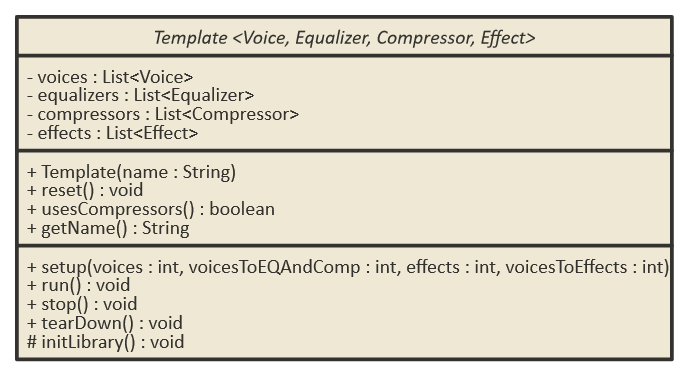
\includegraphics[width=0.5\textwidth]{imgs/nomnoml.png}
  \caption{Klasse diagram van de Template klasse}
  \label{fig:template}
\end{figure}

Figuur \ref{fig:template} toont het klasse diagram van de abstracte en generieke \verb+Template+ klasse van het framework. Dit is de moederklasse van de library specifieke testklasses. Wanneer een klasse zich uitbreid op \verb+Template+, representeert de subklasse een sound synthesis library. De subklasse moet eerst de generieke types \verb+Voice+, \verb+Equalizer+, \verb+Compressor+ en \verb+Effect+ definiëren.

\begin{itemize}
	\item \textbf{Voice} is een oscillatorklasse uit de library.
	\item \textbf{Equalizer} is een klasse uit de library die een inkomende buffer verwerkt. Om trouw te blijven aan de real-life testcases gebruikt men hier best een geluidsfilter. Geluidsfilters hebben karakteristieken van equalizers.
	\item \textbf{Compressor}: idem aan \textbf{Equalizer}.
	\item \textbf{Effect} is nog een verwerkende klasse. Deze klasse representeert een geluidseffect. Bart Vincent en Vagabundos gebruikten vaak een delay effect. \autocite{bartvincent} \autocite{vagabundos} Het wordt aangeraden om een gelijkaardig effect uit de library te kiezen.
\end{itemize}

 In de subklasse worden vervolgens de \verb+setup+-, \verb+run+-, \verb+stop+- en \verb+tearDown+-methode overgeërft. Deze worden als volgt ingevuld.

\begin{itemize}
	\item \textbf{Setup} vraagt de vier parameters uit tabel \ref{tab:parameters}. Aan de hand van deze parameters worden de \verb+Voice+-, \verb+Equalizer+-, \verb+Compressor+-, \verb+Effect+-modules correct geïnstantieerd, geconnecteerd en opgeslagen in de desbetreffende attributen uit de \verb+Template+-klasse.
	\item De \textbf{run}-methode start alle oscillatoren en verwerkende modules die in de \verb+setup+-methode opgesteld zijn. Sound synthesis libraries starten in de meeste gevallen automatisch een nieuwe thread wanneer dit gebeurt. Als dit niet het geval is, moet de ontwikkelaar het zelf in een thread laten uitvoeren\footnote{JASS start bijvoorbeeld geen nieuwe thread wanneer SourcePlayer.start() opgeroepen wordt. Om dit op te lossen werd de PlayThread-klasse ontworpen die de SourcePlayer eenmalig start tot de halt methode opgeroepen wordt.}. Dit is belangerijk voor de performantiemeting. 
	\item De \textbf{stop}-methode stopt de thread - en bijgevolg ook het geluid - die in de \verb+run+-methode opgeroepen is.
	\item \textbf{TearDown} haalt de opstelling van de testcase terug uit elkaar. Voor de modules verwijderd kunnen worden uit het geheugen, moeten ze eerst veilig gedeconnecteerd worden van zowel de library als van de andere componenten. Zo kan de library terug volledig geïnitialiseerd worden voor de volgende testcase.
\end{itemize}

De uit te voeren testklassen en de parameters van de testcases worden statisch bijgehouden in de \verb+StartUp+-klasse. In de \verb+main+-methode wordt per testklasse iedere testcase uitgevoerd. Tijdens het runnen van de audio thread, wordt de performantie van het proces gemeten.

\subsubsection{Performantiemeting van het Proces}

Het voordeel van in een Linux-omgeving te werken is dat er geen externe library nodig is voor de performantiemeting. Alle nodige informatie kan al verkregen worden via het \verb+top+-commando. De taak voor het afnemen van de metingen werd in het framework aan de \verb+Measurer+-klasse gegeven. In die klasse kan commando \ref{command} teruggevonden worden.

\begin{figure}
\centering
\begin{verbatim}
	top -b -n1 -d,01 | \\
	grep %d | \\
	awk '{ if (\$9 != \"0,0\") print \$9 \" \" \$10 }'
\end{verbatim}
\caption{Linux commando om performantie van een proces te meten.}
\label{command}
\end{figure}

\verb+Top+ is een real-time commando. Wanneer het opgeroepen wordt in de terminal, worden alle processen en hun verbruik van CPU en geheugen dynamisch weergegeven. \autocite{topcommand} De volgende vlaggen worden toegepast.

\begin{itemize}
	\item \textbf{-b} start het proces in \textit{Batch mode}. Dit zorgt dat de header met algemene infromatie niet afgebeeld wordt zodat de output beter verwerkt kan worden door andere programma's of commando's.
	\item \textbf{-n1} maakt maar één meting in plaats van een continue dynamische output te geven.
	\item \textbf{-d,01} voert de meting op 0,01 seconden uit.
\end{itemize}

De \verb+-n+-vlag wordt gebruikt omdat Java geen output van dynamische commando's kan lezen. De \verb+-d+-vlag wordt gebruikt zodat de enkele meting zo snel mogelijk gemaakt wordt. Zo doende dook er een probleem op. Wanneer \verb+top+ standaard uitgevoerd wordt, update het proces ongeveer iedere de seconde. Wanneer men de metingen frequenter uit voert, wordt vastgesteld dat de meting voor \verb+%CPU+ onleesbaar is. Ongeveer iedere seconde wordt er een geldige meting afgebeeld. Daartussen vertoont de meting een \verb+0+ als resultaat.

Het interval van de seconde is niet betrouwbaar; soms was het meer, soms was het minder. Daarom wordt iedere 0,01 seconden een meting genomen. Ongeldige metingen worden genegeerd door het programma. Andere metingen worden opgeslaan tot er een totaal van 50 metingen per testcase is. Iedere meting duurt nog steeds ongeveer een seconde, maar van het moment dat een geldige meting verkrijgbaar is, wordt die ook opgenomen. 

De output van het \verb+top+-commando wordt doorgegeven aan het \verb+grep+-commando. Java String formatting maakt gebruik van de \verb|"%d"| om de \textit{process ID} van het framework in te voeren in het commando. Zo verkrijgt men een enkele meting van het gezochte proces. \verb+StartUp+ heeft een statische methode \verb+getPID()+ die de \textit{process ID} van het framework teruggeeft. De output van \verb+grep+ wordt doorgegeven aan het \verb+awk+-commando.

Het \verb+awk+-commando filtert de \verb+%CPU+ en \verb+%Mem+ meting uit de output van \verb+grep+ op voorwaarde dat de \verb+%CPU+-meting geldig is. De output van dit commando wordt ingelezen door Java. De twee metingen worden nog gescheiden door een spatie zodat het makkelijk te verwerken is.

\subsection{Verwerking van de Testresultaten}
\label{sec:methodologie:verwerking}

Per library is er een dataset van 6 testcases. Iedere testcase heeft een subset van 50 metingen. Op zo'n subset wordt eerst een dubbele \textit{moving median} uitgevoerd. \autocite{mediansmoothing} Dit is een smoothing methode waarbij twee keer een nieuwe dataset gemaakt wordt. De nieuwe dataset wordt bekomen door een item te vervangen door de mediaan van zichzelf, zijn voorganger en zijn nakomer; zoals getoond in berekening \ref{math:mediansmooth}. $y_{i}$ is het item van de nieuwe dataset en $x$ representeert de oude dataset. De eerste en laatste waarden worden overgenomen uit de oude dataset omdat berekening \ref{math:mediansmooth} niet mogelijk is op die indexen. Deze dubbele smoothing verwijdert korte periodes van extrema.

\begin{figure}
\centering
$y_{i} = med(x_{i-1}, x_{i}, x_{i+1})$
\caption{\textit{Moving median} formule}
\label{math:mediansmooth}
\end{figure}

De resulterende dataset wordt vervolgens gladgestreken door middel van de Hanning vensterfunctie. Deze functie maakt dat plotse variaties in het frequentiedomein geëgaliseerd worden. Op die manier komen waarden die frequenter voorkomen in de dataset dominanter naar voor. Dit door het lopend gewogen gemiddelde van de waarden in de dataset te berekenen. De Hanning van een waarde in een dataset wordt berekend als de helft van die waarde opgeteld met een kwart van de voorgaande en nakomende meting. Dit staat afgebeeld in berekening \ref{math:hanningformule}. De eerste en laatste waarden van de nieuwe dataset worden overgenomen uit de oude dataset. \autocite{hanning}

\begin{figure}
\centering
$h_{i} = (y_{i-1} + 2 \ast y_{i} + y_{i+1}) \div 4$
\caption{Hanning formule}
\label{math:hanningformule}
\end{figure}

Van de resulterende dataset wordt de mediaan genomen als resultaat voor de testcase. De mediaan is niet gevoelig aan extrema en geeft een betere representatie van de meer frequente metingen in een dataset. \autocite{median} Van de medianen wordt een trendlijn berekend. Zolang de richtingscoëfficient van de trendlijn van de testresultaten niet hoger ligt dan die van het aantal buffers in de input parameters uit tabel \ref{tab:parameters}, kunnen we zeggen dat het technisch aanvaardbaar is om een overstap naar digitaal te maken. 

\section{Emotionele tests}
\label{sec:methodologie:emotioneletests}

Na de technische bespreking van de muzikale opstellingen van de interviewees, werden volgende vragen gesteld:

\begin{itemize}
	\item Is er potentie voor digitalisering in de muziekindustrie?
	\item Wie zou hier het meeste baat bij hebben?
	\item Wie zou hier het meeste interesse in hebben?
	\item Zou een digitalisering verwelkomd worden in de sector?
\end{itemize}

Op basis van deze vragen, weten we of de branche van dat profiel in de muzieksector open staat voor een digitalisatie.

Er zijn door tijdsgebrek en de kleine respons (zie tabel \ref{table:correspondentie}) slechts vier interviews afgenomen. Dit is duidelijk te weinig data om een populatie te representeren.

Iedere interviewee beeld een profiel uit zoals in tabel \ref{tab:profielen} staat. Als resultaat op de emotionele test van een profiel wordt uit belang van dit onderzoek het resultaat van de interviewee zelf genomen.

\iffalse \lipsum[21-25] \fi


\chapter{Verloop van het Onderzoek}
\label{onderzoek}

\section{Is het mogelijk om digitaal te gaan?}
\label{onderzoeksvraag1}

Deze sectie gaat na welke methode van geluidsverwerking het best toegepast wordt bij het schrijven van verwerkingsprogramma's. Uit het interview van \textcite{thomashouthave} bleek dat hij het meest intuïtief overweg gaat met subtractive synthesis. In sectie \ref{methode:subtractive} wordt besproken hoe deze methode werkt. \textcite{thomashouthave} meldt in zijn interview dat equalizers en compressors een uitwerking van subtractive synthesis zijn. De andere interviewees vermeldden ook dat zij extensief gebruik maken van equalizers en compressors. Het artikel van \textcite{filtervseq} biedt hier meer inzicht op.

\subsection{Geluidsfilters}

Filters maken prominent deel uit van de subtractive methode zoals in sectie \ref{methode:subtractive} beschreven staat. \textcite{filtervseq} spreekt over de gelijkenissen en verschillen tussen audio equalization en filtering. Waar equalizers bepaalde delen van het frequentiespectrum van een geluid versterken, knippen filters ze af. Beide kunnen gebaseerd worden op een Fast Fourier Transformatie (FFT)\footnote{\textit{fouriereq} leggen in hun onderzoek een toepassing van equalizers uit voor gehoorapparaten. Het idee is om een equalizer in gehoorapparaten te implementeren die bepaalde frequenties verluidt. Die frequenties worden gekozen op basis van het audiogram van de patient. Een audiogram geeft weer vanaf welke amplitude een patient een zekere frequentie kan horen. Zo worden enkel de moeilijk te horen frequenties versterkt. Dit wordt verwezenlijkt door middel van FFT.}. Het enige verschil tussen de twee is de amplitudinale impact. Een equalizer versterkt het geluid rond een zekere frequentie terwijl een filter het verzacht.

Niet alleen biedt FFT meerdere toepassingen in subtractive synthesis. Het biedt ook een tijdscomplexiteit van $\mathcal{O}(n\log{}n)$ die meer acceptabel is dan die van de Discrete Fourier Transformatie (DFT) van $\mathcal{O}(n^2)$.\autocite{ffttime} Het is niet optimaal, daarom worden er reeds tal van onderzoeken gevoerd om de tijdscomplexiteit te verminderen in software aan de hand van multicore computing. \autocite{robbievincke}

De bespreking van FFT is ter illustratie dat equalizers gebaseerd zijn op subtractive synthesis. Er zijn tal van toepassingen van FFT in geluidsfilters. FFT is in software typisch niet de verkozen transformatie omdat het bedoeld is voor de spectroscopie van frequenties van continue signalen. De sound synthesis libraries besproken in sectie \ref{sec:libraries} maken hier gebruik van de bilineaire tranformatie \autocite{jsynbiquad} omdat die beter toepasbaar is op de real-time verwerking van discrete signalen\footnote{\textcite{rbj} bespreekt in zijn artikel zijn algoritme voor de bilineaire transformatie.}. \textcite{rbj} toont in zijn artikel hoe verschillende filter types geïmplementeerd kunnen worden aan hand van deze transformatie.

\subsection{Harmonisch rijke golven}

Op eerste zicht lijkt het per definitie onmogelijk voor een computer om harmonisch rijke golven te genereren. \textcite{fourier} vertellen het verhaal van Joseph Fourier. Hij hypothiseerde in de 19\textsuperscript{de} eeuw dat alle periodieke functies beschreven kunnen worden als een oneindige som van sinusfuncties - vandaar de benoeming \textit{harmonisch rijk}. Twee jaar voor zijn dood, in 1828, werd dit bewezen door Johann Dirichlet, een wiskundige met wie Fourier correspondentie voerde. Het zijn deze periodieke golven waar subtractive synthesis zich op baseert. \autocite{fourier}

\begin{figure}
\centering
\begin{verbatim}
Function<double, double> square = x -> (x % f) < f / 2 ? -1 : 1;
\end{verbatim}
\caption{Java blokgolf generatie functie}
\label{squarefunction}
\end{figure}

Per definitie is het computationeel onmogelijk om een oneindige som van sinusfuncties te genereren.  Maar in se is dat ook niet nodig. Evenals analoge synthesizers genereren de libraries uit \ref{sec:libraries} hun harmonisch rijke golven door middel van logica in plaats van trigonometrie. Zo kan de generatie van een harmonisch rijke functie vaak ondergebracht worden in één bewerking. Een voorbeeld: functie \ref{squarefunction} genereert een blokgolf van frequentie \verb+f+ gegeven een abcis \verb+x+.



% Voeg hier je eigen hoofdstukken toe die de ``corpus'' van je bachelorproef
% vormen. De structuur en titels hangen af van je eigen onderzoek. Je kan bv.
% elke fase in je onderzoek in een apart hoofdstuk bespreken.

%\input{...}
%\input{...}
%...

%%=============================================================================
%% Conclusie
%%=============================================================================

\chapter{Conclusie}
\label{ch:conclusie}

% TODO: Trek een duidelijke conclusie, in de vorm van een antwoord op de
% onderzoeksvra(a)g(en). Wat was jouw bijdrage aan het onderzoeksdomein en
% hoe biedt dit meerwaarde aan het vakgebied/doelgroep? 
% Reflecteer kritisch over het resultaat. In Engelse teksten wordt deze sectie
% ``Discussion'' genoemd. Had je deze uitkomst verwacht? Zijn er zaken die nog
% niet duidelijk zijn?
% Heeft het onderzoek geleid tot nieuwe vragen die uitnodigen tot verder 
%onderzoek?

\section{Is het mogelijk om digitaal te gaan?}

Uit sectie \ref{onderzoeksvraag1} bleek dat het wel degelijk mogelijk zou zijn om digitaal te gaan. Er bestaat al technologie voor, het moet enkel nog correct geïmplementeerd worden. De correcte implementatie is hier van essentie, zoals bij de testresultaten van JASS te zien was.

Dat niet alleen. Op dit moment wordt er meer onderzoek gevoerd naar toepassingen van andere methodes van digitale geluidsgeneratie zoals granular en wavelet synthesis. Houthave zei in zijn interview: \textit{``granulaire synthesis is dan weer muzikaler van aard. Daar definieer je instrumenten.''} \autocite{thomashouthave} Dit onderzoek heeft zich beperkt tot subtractive synthesis omdat het de meest intuïtieve generatie- en verwerkingsmethode is voor het doelpubliek. \textcite{granular} legt in zijn paper een methode voor real-time granular synthesis uit. Zoals in sectie \ref{methode:granular} staat moet hier een groot aantal parameters bediend worden dat toeneemt naargelang de complexiteit van het geluid. Daarbij is \textit{simplicity key} voor een product dat aan de consument verkocht wordt. Hier kan zeker verder onderzoek gevoerd worden.

User interfaces vallen buiten de scope van dit onderzoek. Voor verdere ontwikkeling is belangerijk dat de profielen live slechts één parameter op eenzelfde moment bedienen. Met toetsenbord en muis is het zeker haalbaar om de bediening van één parameter uit te voeren.

\section{Is het nuttig om digitaal te gaan?}

Sectie \ref{onderzoeksvraag2} toonde aan dat alle profielen een digitale transitie zouden verwelkomen. Wat opvalt is dat sommige profielen bepaalde eisen stellen voor het eindproduct. Zo eisen muzikanten om het taktiele in hun instrument te behouden en hebben producers nood aan een hogere geluidsresolutie dan standaard CD-kwaliteit. Zolang aan die wensen voldaan kan worden, is er interesse naar digitalisatie op de markt.

Of de consumenten er direct positief op gaan reageren is een ander verhaal. Vincent en Boone zien veel potentieel in digitale verwerking voor live muziek. Voornamelijk omdat digitaal het werkproces versnelt en vergemakkelijkt. Toch blijft Boone sceptisch over de digitale transitie. Ten eerste omdat de genres van zijn klanten niet thuis horen in een digitaal milieu en ten tweede omdat de digitale tafels van vandaag geen deftige geluidsresolutie kunnen verwerken. Er is dus zeker vraag naar digitale mengtafels die hogere geluidsresoluties dan \textit{standaard CD-kwaliteit} \autocite{peterboone} aankunnen.

Uit andere interviews en uit \ref{onderzoeksvraag1} bleek echter dat er geen hoorbaar verschil is tussen digitaal en analoog. Natuurlijk zal analoge verwerking altijd wat ruis en vuil hebben. Sommige artiesten en producers zijn hier net naar opzoek. \textit{``Iemand kan vinden dat digitaal veel cleaner is. Anderen vinden dat ze karakter missen. Maar veel van dat "vuil" kan ook gegenereerd worden door een plugin,''} vertelt Vincent over digitale of analoge voorkeuren. \autocite{bartvincent} 

Boone vertelt na zijn interview over een fout die hij in een track van de Beatles gehoord heeft. Het is algemeen geweten dat er zich veel foutjes in de albums van de Beatles verschuilen. Dat zijn dingen die niet meer kunnen in de muzieksector van vandaag. Een song moet een afgewerkt product zijn, zonder vuil of fouten. Daar kan digitaal zeker bij helpen, zegt Boone. \textit{``Dat is wel een voordeel van digitaal ten opzichte van analoog. Als je bij analoog een te laag opnameniveau hebt en je trekt het op, dan trek je ook de ruis op. En digitaal heeft geen ruis.''} \autocite{peterboone}

Een andere manier om deze vraag te beantwoorden is door te kijken naar de voordelen die digitaal ten opzichte van analoog heeft.

\begin{itemize}
	\item Het opslaan van instellingen en die met een druk op de knop terug kunnen inladen.
	\item Het standaardiseren van die digitale instellingen zodat ze tussen opstellingen en artiesten gedeeld kunnen worden.
	\item De prijs die significant lager ligt in vergelijking met de analoge varianten.
	\item De compactheid van het product.
	\item Digitaal is \textit{cleaner} en bevat geen ruis.
\end{itemize}

Hieruit wordt geconcludeerd dat het algemeen zeker nuttig is om digitaal te gaan. Maar daarmee is niet aan de wensen van ieder profiel voldaan. In sectie \ref{endeontwikkelaars} wordt hier dieper op ingegaan.

\section{Is het realistisch om digitaal te gaan?}
\label{conclusie3}

Om deze vraag te beantwoorden moest slechts één van de libraries een goede performantie vertonen. Pas dan mocht gezegd worden dat het realistisch is om digitaal te gaan. In sectie \ref{onderzoeksvraag3} werd aangetoond dat JSyn alle testcases aankon. Dus wordt geconcludeerd dat het realistisch is om digitaal te gaan.

Voor een open-source Java library heeft JSyn goed gescoord op de empirische test. Maar wanneer puntje bij paaltje komt, zal het eindproduct niet met JSyn geschreven worden. Bedenk dat de empirische tests afgenomen zijn op een particuliere laptop. De laptops verkrijgbaar op de hedendaagse markt zijn veel sterker dan onze testmachine. Bedenk hoe een C++-library zou presteren. Zulke low-level programmeertalen presteren zeker beter dan Java.  

\section{Wat wilt dit zeggen voor ontwikkelaars?}
\label{endeontwikkelaars}

\begin{table}[]
\begin{tabular}{l|l|l|l|}
\cline{3-4}
\multicolumn{2}{l}{\multirow{2}{*}{}}  & \multicolumn{2}{c|}{\textbf{Empirische tests}}                                                                                                                  \\ \cline{3-4} 
\multicolumn{2}{l}{}   & \textbf{Positief} & \textbf{Negatief} \\ \hline
\multicolumn{1}{|l|}{\multirow{2}{*}{\textbf{Emotionele tests}}} & \textbf{Positief} & Betreed de markt.                                                                           & \begin{tabular}[c]{@{}l@{}}Er is interesse maar\\ het is technisch niet mogelijk.\end{tabular} \\ \cline{2-4} 
\multicolumn{1}{|l|}{}                                           & \textbf{Negatief} & \begin{tabular}[c]{@{}l@{}}Het is technisch mogelijk\\ maar weinig vraag naar.\end{tabular} & \begin{tabular}[c]{@{}l@{}}Slecht idee om de markt\\ te betreden.\end{tabular}                 \\ \hline
\end{tabular}
\caption{Uitkomsten van de Emotionele-Empirische test.}
\label{EEtest}
\end{table}

Tabel \ref{EEtest} geeft beter inzicht in de situatie. JSyn scoorde positief op onze empirische tests. In sectie \ref{conclusie3} wordt besproken dat alternatieve manieren van geluidsgeneratie en -verwerking betere prestaties opleveren. Het is technisch zeker mogelijk om de overstap naar digitaal te maken. De emotionele tests, daarentegen, zijn afhankelijk van profiel tot profiel. Waar de digitalisatie gegeerd is voor sound designers, geluidstechnici en sommige muzikanten, is dat niet altijd het geval bij producers en opname artiesten.

Het is technisch zeker mogelijk om de digitale transitie te maken. Uit de interviews bleek bovendien dat daar ook interesse voor is. Dus als hier verdere ontwikkelingen gebeuren - rekening houdend met profielspecifieke requirements - maakt de ontwikkelaar kans in de markt.

\section{Toekomstig Onderzoek}

\subsection{Grotere Bevraging}

Dit onderzoek geeft een duidelijke indicatie dat er ruimte is voor ontwikkelaars in de markt. Een bredere bevraging van de muzieksector is wenselijk om de requirements van de profielen te verfijnen.

\subsection{Proof-of-concept}

Toekomstig onderzoek kan proberen om digitale versies te maken van analoge apparatuur. Denk hierbij aan mengpanelen, voorversterkers, effectpedalen, synthesizers, direct input boxes etc. Bij voorkeur worden deze in een low-level programmeertaal geschreven, onafhankelijk van een library en met een minimalistische user interface.

\subsection{Alternatieve Methodes voor Geluidsgeneratie en -verwerking}

In sectie \ref{sec:methodesgeneratie} werden verschillende methodes voor geluidsgeneratie en -verwerking besproken. Met name granular, wavelet en corpus-based granular synthesis. Toekomstig onderzoek kan op zoek gaan naar efficiente manieren om deze methodes toe te passen in verwerking en generatie van muziek. Dat niet alleen. Thomas Houthave sprak in zijn interview over toepassingen van AI in het simuleren en immiteren van geluid. Hier ziet hij tepassingen voor in sound design voor game engines. \autocite{thomas houthave} Hij sprak ook over \textit{bionische muzikanten} die jammen met een artiest. Het programma speelt in op noten of akkoorden die de muzikant speelt. Zo kan de muzikant begeleid worden in het creëren van zijn muziek.

\iffalse \lipsum[76-80] \fi



%%=============================================================================
%% Bijlagen
%%=============================================================================

\appendix
\renewcommand{\chaptername}{Appendix}

%%---------- Onderzoeksvoorstel -----------------------------------------------

\chapter{Onderzoeksvoorstel}

Het onderwerp van deze bachelorproef is gebaseerd op een onderzoeksvoorstel dat vooraf werd beoordeeld door de promotor. Dat voorstel is opgenomen in deze bijlage.

% Verwijzing naar het bestand met de inhoud van het onderzoeksvoorstel
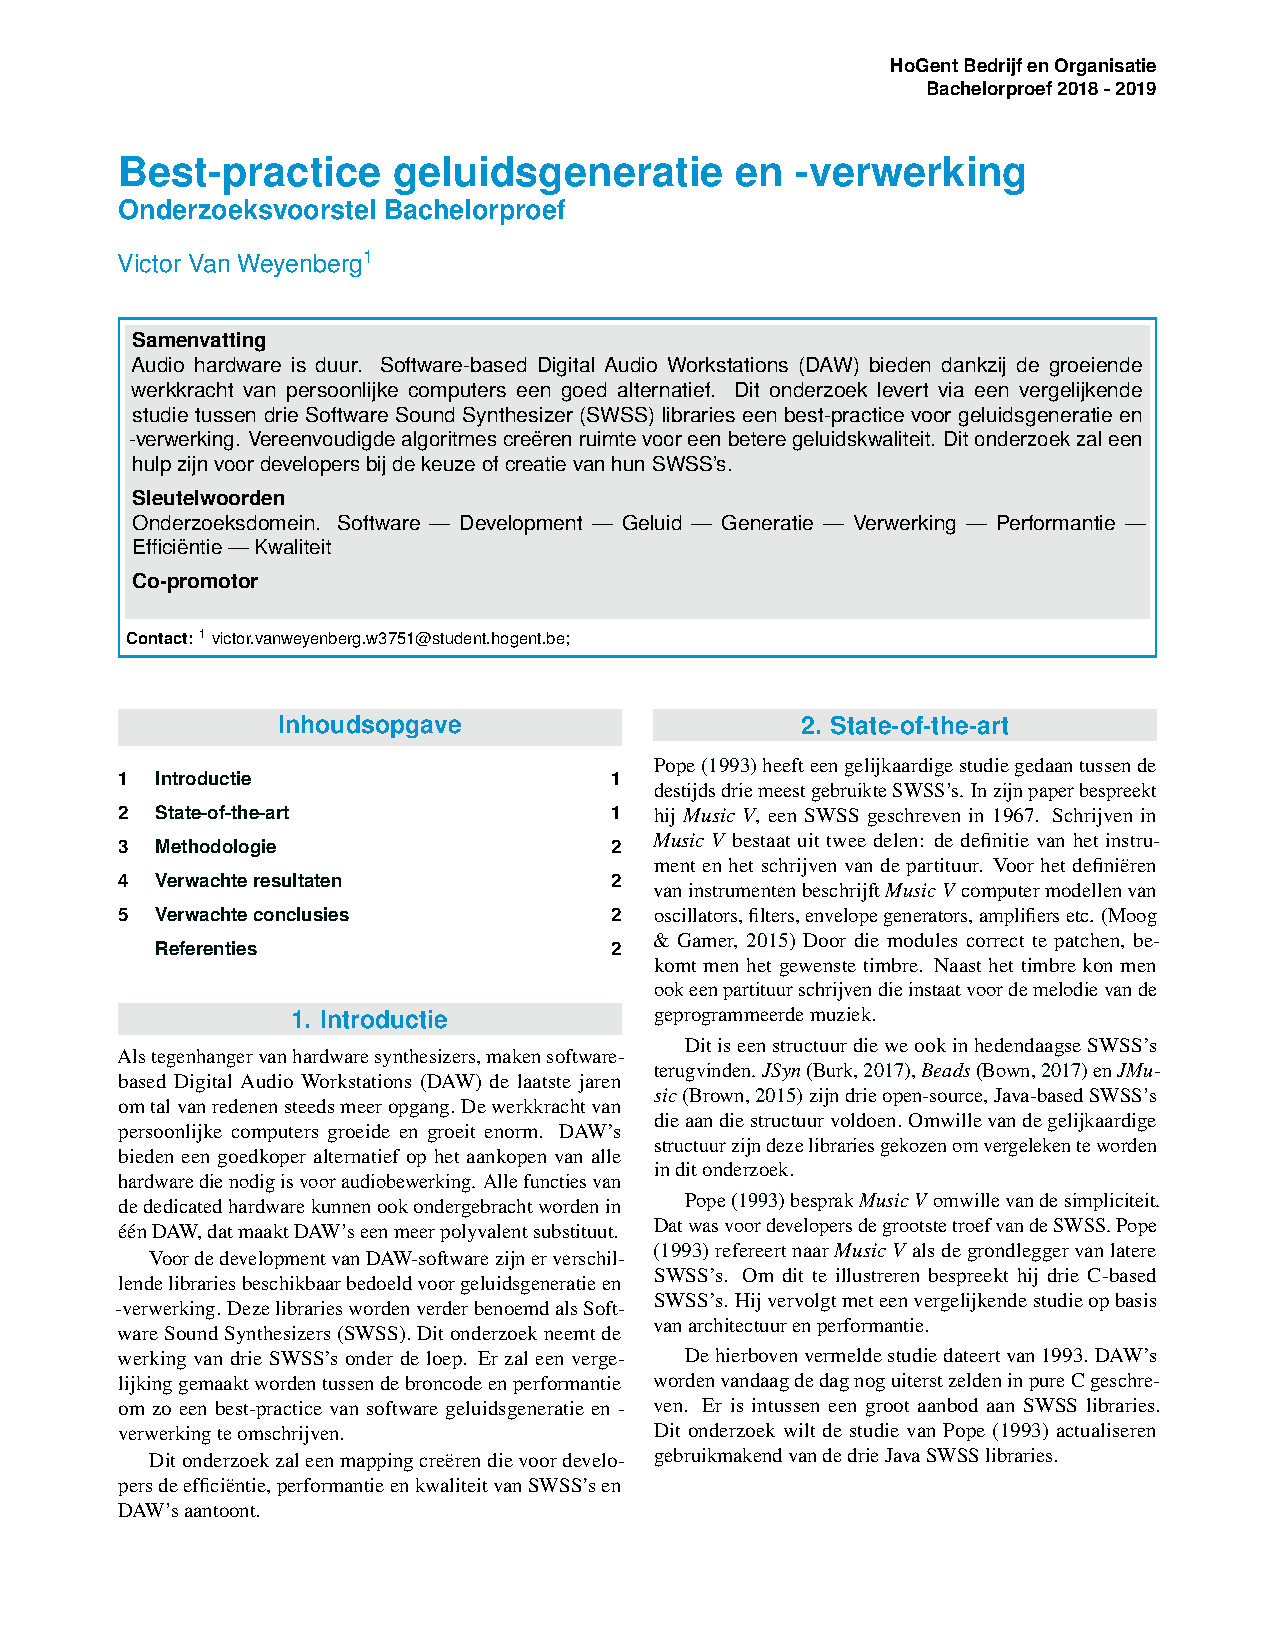
\includepdf[pages=-]{Voorstel_2018___2019.pdf}

%%---------- Andere bijlagen --------------------------------------------------
% TODO: Voeg hier eventuele andere bijlagen toe
%\input{...}

\begin{table}[h!]
  \centering
  \begin{tabular}{|l|l|}
    \hline
    \textbf{Naam} & \textbf{Functie} \\
    \hline
    Babek Joshghani & Dub artiest \\
    \hline
    Radio 2 & Radio zender \\
    \hline
    Colin Benders & Electro artiest \\
    \hline
    UrgentFM & Radio zender \\
    \hline
    BOMA studio & Opname studio \\
    \hline
    Vagabundos & Band \\
    \hline
    JARVIN & Band \\
    \hline
    ROOM13 & Opname studio \\
    \hline
    Peter Moorkens & Electro artiest \\
    \hline
    House of Media & Opname studio \\
    \hline
    Peter Van Praag & DJ \\
    \hline
    Muziekcafé Charlatan & Muziek café \\
    \hline
    Muziekcentrum Kinky Star & Muziek café \\
    \hline
    Hypestudio & Opname studio \\
    \hline
    Ben Van Camp & Muzikant \\
    \hline
    Muziekcentrum Goed Leven & Opname studio \\
    \hline
    Dante van Quaethem & Hoofdtechnicus Kinky Star \\
    \hline
    Frederik Sioen & Band \\
    \hline
    Mathias Sercu & Acteur / Muzikant \\
    \hline
    Bart Vincent & Producer \\
    \hline
    Thomas Van Elsander & Gitarist  \\
    \hline
    Thomas Houthave & Geluidsingenieur \\
    \hline
    Frank Dûchene & Producer \\
    \hline
    Stijn & Artiest \\
    \hline
    Peter Boone & Opname artiest \\
    \hline
  \end{tabular}
  \caption{Lijst van correspondenten en hun functies.}
  \label{table:correspondenten}
\end{table}

\begin{landscape}
\begin{table}
  \centering
  \begin{tabular}{|l|l|l|l|l|}
    \hline
    \textbf{Naam} & \textbf{Datum} & \textbf{Medium} & \textbf{Beschrijving} & \textbf{Resultaat} \\
    \hline
    Babek Joshghani & 27/03/2019 & Telefoon & Vraag voor interview & Overgaan op mail conversatie \\
    \hline
    JARVIN & 28/03/2019 & Telefoon & Vraag voor interview met Vagabundos & Doorverwijzing naar JARVIN \\
    \hline
    Babek Joshghani & 28/03/2019 & E-mail & Vraag voor interview & Interview vastgelegd \\
    \hline
    ROOM13 & 28/03/2019 & Website & Vraag voor interview &  \\
    \hline
    Colin Benders & 28/03/2019 & E-mail & Vraag voor interview &  \\
    \hline
    Radio 2 & 28/03/2019 & E-mail & Vraag voor interview &  \\
    \hline
    UrgentFM & 28/03/2019 & E-mail & Vraag voor interview &  \\
    \hline
    BOMA studio & 28/03/2019 & E-mail & Vraag voor interview &  \\
    \hline
    Frederik Sioen & 28/03/2019 & Facebook & Vraag voor interview &  \\
    \hline
    Radio 2 & 01/04/2019 & E-mail & Extra uitleg geven over interview. &  \\
    \hline
    JARVIN & 02/04/2019 & Telefoon & Tweede vraag voor interview & Interview vastgelegd \\
    \hline
    Babek Joshghani & 02/04/2019 & E-mail & Tweede vraag voor interview & In overleg \\
    \hline
    Ben Van Camp & 06/04/2019 & Telefoon & Vraag voor interview & In afwachting van antwoord \\
    \hline
    Peter Moorkens & 06/04/2019 & E-mail & Vraag voor interview &  \\
    \hline
    House of Media & 06/04/2019 & E-mail & Tweede vraag voor interview &  \\
    \hline
    Peter Van Praag & 06/04/2019 & Telefoon & Vraag voor interview & Interview vastgelegd \\
    \hline
    Muziekcentrum Goed Leven & 06/04/2019 & Telefoon & Vraag voor interview & Bericht achtergelaten op het antwoordapparaat \\
    \hline
    Muziekcentrum Kinky Star & 06/04/2019 & Telefoon & Vraag voor interview & Doorverwijzing naar hoofdtechnicus Dante van Quaethem. \\
    \hline
    Dante van Quaethem & 06/04/2019 & E-mail & Vraag voor interview &  \\
    \hline
    Hypestudio & 06/04/2019 & Website & Vraag voor interview &  \\
    \hline
    Mathias Sercu & 08/04/2019 & Telefoon & Vraag voor interview, ook voor broers & Doorverwijzing naar Thomas Van Elslander en Thomas Houthave \\
    \hline
    Bart Vincent & 08/04/2019 & Telefoon & Vraag voor interview & Interview vastgelegd \\
    \hline
    Thomas Houthave & 08/04/2019 & Telefoon & Vraag voor interview & Interview vastgelegd \\
    \hline
    Thomas Van Elsander & 08/04/2019 & Telefoon & Vraag voor interview & Voicemail achtergelaten. \\
    \hline
    Ben Van Camp & 08/04/2019 & Telefoon & Vraag voor interview & Overgaan op e-mail correspondentie \\
    \hline
    Ben Van Camp & 08/04/2019 & E-mail & Vraag voor interview &  \\
    \hline
    Stijn & 09/04/2019 & E-mail & Vraag voor interview &  \\
    \hline
    Frank Dûchene & 09/04/2019 & E-mail & Vraag voor interview &  \\
    \hline
    Peter Boone & 17/04/2019 & Facebook & Vraag voor interview & Interview op 24/04 \\
    \hline
    Peter Moorkens & 24/04/2019 & E-mail & Verdere planning interview & Geen antwoord \\
    \hline
    Babek Joshghani & 24/04/2019 & Telefoon & Verdere planning interview & Geen antwoord \\
    \hline
  \end{tabular}
  \caption{Lijst van correspondentie met datum, medium, beschrijving en resultaat van het bericht.}
  \label{table:correspondentie}
\end{table}
\end{landscape}
\chapter{Transcripties van de interviews}

\section{Bart Vincent (Producer)}
\label{trans:bartvincent}

\textbf{Dus over de digitalisatie?}\newline
Dat is nu al bezig. Ik ben opgegroeid met analoge mengtafels, live. Er bestond toen een digitale tafel en die was *kut* eigenlijk. Maar die kon heel veel al op die momenten.
Nu wilt niemand daar nog op werken omdat die pre-amps zo slecht zijn eigenlijk. Intussen is er zoveel geëvolueerd.
In die tijd kreeg je een analoge mengtafel. Als er na u nog een band moest soundchecken moest je alles overschrijven.
Van elke tafel kon je script sheets downloaden, daarop kon je aanduiden hoe de queues stonden.
Intussen kom je bijna geen analoge tafels meer tegen.
Laatste vier jaar ben ik live maar 4 analoge tafels tegengekomen.
Hoe meer je de tafels leert kennen hoe meer je ermee overweg kan.

\textbf{Mijn idee was dat alles nog analoog verliep.}\newline
Alles? Dat niet nee. Maar de stage blocks, micro's etc. Die verlopen nog altijd via een kabel, dat is analoog.
Maar ze worden aangesloten op een digitale mengtafel.

\textbf{Is die digitale mengtafel dan gewoon een computer?}\newline
Nee, het is een computer waarbij de schuivers een tool zijn die een computer aansturen.
Na het selecteren van een track stel je de instellingen van die track in aan de hand van één input.

\textbf{Al die stemmen worden allemaal verwerkt door de computer?}\newline
Ja, er verloopt altijd een analoog/digitaal conversie.

\textbf{Klopt het dat, afhankelijk van de kwaliteit van de conversie, digitaal geluid slechter klinkt?}\newline
Nee, ik denk dat niet. Vroeger nam je op een band. Hoe breder uw band, hoe meer informatie je erop op kan slaan. De breedte kan je nu vergelijken met de 16- of 24-bit range van de geluidskwaliteit. Het is de hoeveelheid van 0'etjes en 1'tjes die je kan opslaan die maken hoe definieert uw geluid is.
Ook de snelheid van de tape is belangrijk. Het aantal samples per seconde. En zeker belangrijk is de klok. Als je een accurate klok hebt, zal die de juiste samples op het juiste moment afspelen. Je kan soms enorm dure machines hebben die enkel dienen om een klok te genereren. Dat communiceert met uw DAW en dat zorgt dat uw soundbytes op het juiste moment gegenereerd worden.

\textbf{Je werkt live; hoeveel stemmen gebruik je?}\newline
Ik werk op een beperkte versie van Protools, daar ben je gelimiteerd tot 128 tracks.

\textbf{Gebruik je meer?}\newline
Nee, als je meer zou gebruiken, zou je al direct met een orkest samen werken. Als je een gewone pop band opneemt zou je genoeg hebben met zo'n 50-tal tracks.

\textbf{Welke tracks zijn dat dan?}\newline
Een aantal voor doubling via een andere microfoon voor een andere kleurklank. Verder kan je als snel aan 12 kanalen komen met een drum kit.

\textbf{Je bent een grote voorstander van zo min mogelijk postproductie te doen.}\newline
Ja. Iedereen moet aangevoerd worden. Als je een tom hebt die iet goed gestemd is, dan zit het in alle microfoons. Je kan sound replacement doen maar ik ben een voorstander van al te zoeken naar de klank die je wilt hebben in de studio, alvorens je gaat opnemen.

\textbf{Ik zoek naar het real-time aanpassen van geluid. Wat doe je daar op een podium? Werk je constant met een heleboel parameters? Zijn dat er enkelen?}\newline
Alles wordt gesoundcheckt, het hele team wordt aangevoerd. Melanie Debiasio zingt van nature zeer stil. Als er dan een instrument te luid speelt dan communiceer ik dat ook. Als hij te luid speelt, komt dat in de micro van Melanie omdat die zo luid staat.
Maar waar ik bijstuur, ik queue, ik compress.
Met digitale mengtafels kan je alles al op voorhand instellen.

\textbf{Hoeveel effecten gebruik je zo per track?}\newline
Ik zet er standaard 5 klaar.

\textbf{Wat is jouw creatieproces?}\newline
Ruimte controleren, band en zangeres placeren. Maken dat iedereen zijn klank overeen komt hoe zij het willen. Dan is er een PA-repetitie; een generale repetitie met alle technici.

\textbf{Is er een good-practice in jouw vak?}\newline
Er zijn een aantal regels. Natuurlijk kan je met digitaal niet in het rood gaan. Op een analoge tafel kan dat een leuk effect hebben.

\textbf{En wat is het meeste werk tijdens het optreden zelf?}\newline
Ik luister. Soms stuur ik wat bij als het nodig is zodat alles overkomt zoals het hoort.

\textbf{Is er ruimte voor automatisatie?}\newline
Onmogelijk, dat is allemaal afhankelijk van smaak. En iedereen heeft een andere smaak. Er is een plugin genaamd Izotope-8 die de gebruiker een mix voorstelt zodat het klinkt zoals een referentietrack. Maar dan kies jij, als gebruiker nog steeds of je het goed vindt of niet.
Het hangt ook af van de ruimte. De charlatan gaat anders klinken dan het sportpaleis.
Slates maakt een microfoon waarbij de karakteristieken van de microfoon digitaal kan instellen. Ik geloof het zelf niet want volgens mij werkt een groot membraan microfoon nog steeds met een groot membraan. Maar zo zijn er plugins, van verschillende merken, die zeker analoge pre-amps simuleren. En dat komt zeer dicht in de buurt.
Ik heb verschillende pre-amps zowel analoog als digitaal gehoord en als je blind luisters zou ik niet kunnen zeggen welke hardware en welke software was.

\textbf{Zijn er special technieken die eigen zijn aan jou?}\newline
Distortion om harmonieën bij te brengen.

\textbf{Waarom hangen zoveel mensen vast aan analoog? Waarom maken ze de overstap naar digitaal niet ookal klinkt het hetzelfde?}\newline
Dat heeft te maken met smaak. Ik heb u gesproken over Peter Klaas. Ik ben bij hem op cursus geweest. Daar hoorden we twee keer hetzelfde nummer. éénmaal bewerkt met digitale gear; andere keer bewerkt met analoge gear.
Een iemand kan vinden dat digitaal veel cleaner is. Anderen vinden dat ze karakter missen. Maar veel van dat "vuil" kan ook gegenereerd worden door een plugin.
Het feit dat iets imperfect is maakt dat je soms tot iets onbedoelds maar origineels komt. Daar zoek je in productie soms wel naar.

\textbf{Gebruik je soms andere manieren van geluidsgeneratie?}\newline
Nee.

\textbf{[Ik geef een uitleg over verschillende soorten generatie.]\newline
In welke methode past jouw vak het best?}\newline
Ik ben een man van compressie en equalizing. Mijn geluiden moeten passen in een geheel. Zo lijkt het het best op subtractive synthesis.
Wat ik ook wel doe is veel doubling, het creëren van een "wall of sound". Doubling is twee keer hetzelfde proberen spelen. Het is onmogelijk om twee keer hetzelfde te spelen dus de kleine afwijkingen in het geluiden maken dat het veel vetter gaat klinken.

\textbf{Is het mogelijk om digitaal te gaan?}\newline
Ik denk dat het nu al gebeurt. Dus ja! Zeker. In mijn leefwereld heeft alles te maken met de afstelling van de artiest. Dus of het allemaal goed gaat klinken, weet ik niet.

\textbf{Wie zou er baat bij hebben?}\newline
Amateurs. Als je in een vlugge flow zit op radio, zou het zeker ook kunnen. Digitale gitaarpedalen bestaan al, Line Six is daarmee begonnen. Radio Head genereert zelf ook zijn eigen effecten.
De verwantschap met het instrument gaat anders zijn, maar het gaat nogsteeds een instrument zijn waar je mee om kan leren gaan.
Het fysieke gaat het meest gemist worden. Het is de look-and-feel die de muzikale ervaring versterkt.

\textbf{Waarom zou digitalisering niet verwelkomd worden?}\newline
Het wordt wel verwelkomd maar een computer gaat gewoon nooit het werk van een mens kunnen overnemen.
De tools, die de mensen helpen bij hun job, die worden wel beter.

\section{Peter Boone (Producer en Muzikaal Artiest)}
\label{trans:peterboone}

\textbf{Hoe benoemt u uw functie in de muzieksector?}\newline
Muzikant, arrangeur, producer. Maar voornamelijk auteur componist. Het deel productie is ondergeschikt maar noodzakelijk. Ik wou niet afhankelijk zijn dus heb ik het mezelf aangeleerd.

\textbf{Wat voor projecten heeft u zoal?}\newline
Het meest bekende is Split Second. Een Electronic Body Music Group (EBM) die in de jaren '80 mondiaal succes gehad heeft. We hebben wereldwijd in de top 10 gestaan en een LP of duizend verkocht in Amerika.

\textbf{U heeft een uitgesproken mening over de digitalisering. Wat is uw creatieproces?}\newline
Hangt af van de context. Als ik een song schrijf komt eerst de tekst.
Dan probeer ik het te accompagneren door ofwel piano ofwel tekst. Soms ontstaat het ook uit een bass-riff of een loopje.
En voor je het weet heb je een song. En dat komt zeer organisch tot stand.
Ik heb ondertussen zowel de digitale als analoge werkwijze toegepast en die werkwijze is eigenlijk niet veranderd.
Ik maak het zeer organisch tot ik tevreden ben. Wanneer het stuk volledig naar mijn hand staat, noem ik het een afgewerkt product.
Soms heb ik tracks teveel maar dan moet ik er later uitknippen. Less is more in productie.
Een arrangeur bouwt op in zijn productie en een producer die schaaft het dan af tot een afgewerkt product.

\textbf{Op dit moment, bent u digitaal of analoog bezig?}\newline
Ik heb er verschillende fasen in. Op het moment dat de digitalisering begon kon het niet digitaler zijn.
Ik heb momenten gehad dat ik het ambetant vond dat zelfs een microfoon nog analoog was.
Omdat, zeker als je niet in de top budgetten zit ga je sneller een goed resultaat behalen met digitale apparatuur dan met analoge apparatuur.
Maar ondertussen heb ik geïnvesteerd in van alles en nog wat en heb ik gemerkt dat digitale mengtafels het eerste is dat ik heel zwak vindt.
Vreselijk ontgoochelend van klank. Dat is het eerste dat ik uit mijn opstelling gezwierd heb. Maar dan moet je wel geld bovenhalen.
Goedkope analoge mengtafels trekken op niks, hebben ook geen equalizers. Maar in de prijsklasse van 10-20 duizend euro kom je wel bij analoge mengers die beter zijn alles wat je op de markt vindt.
Er is een heel vreemde stagnatie in digitale mengers. Zelfs de heel dure modelllen van sound craft werken nog altijd op een sample frequentie van 44.1 Hz en dat vind ik gewoon niet goed.
44.1 is CD niveau en de klank van een CD is beschamend slecht, nauwelijks beter van een cassetje.

\textbf{Er is daar dus een grote tekortkoming?}\newline
Ja, absoluut, ik zit nog altijd te wachten op het volgende formaat, namelijk 88.2 en 24-bit. De CD is 44.1 en 16-bit. Eender wat je daar van subtiliteit in wilt steken gaat verloren omdat de notatie niet goed genoeg is.
Eens je daar naar 88.2 gaat, wordt een galm terug een ruimte in plaats van een effectje. en als je analoog blijft, heb je dat probleem natuurlijk niet.

\textbf{Waarom zou het moeilijk zijn om over te stappen naar 88.2?}\newline
Ik vraag het me ook af. Ik weet het niet. Maar zelfs de echt dure mengers zoals de VI-4 van Sound Craft die toch de standaard digitale menger aan het worden is in het digitale milieu is 44.1 Hz.
Pas op, Yamaha biedt wel menger aan die 88.2 en zelf 192 Hz aankunnen. Maar die zijn lang niet zo verspreid als andere mengers.

\textbf{Zou dat liggen aan een standaardisatie?}\newline
Ja, natuurlijk, dat zal het wel zijn. Er is live en er is studio, dat zijn twee verschillende dingen. Als je mij live zou vragen wat ik vind van digitalisatie, dan noem ik het perfect.
Daar zijn er geen analoge mengers meer. Alles werkt veel sneller, je kan ook zekere settings automatisch oproepen. Dat werkt ongelooflijk professioneel.
Maar in de studio heb je wel tijd, en daar klinkt het beter als je het zo lang mogelijk analoog werkt en pas op het laatste moment overstapt op digitaal.

\textbf{Leg eens verder uit hoe de werkwijze van analoog naar digitaal producen niet veranderd is.}\newline
Dezelfde regels gelden voor beiden. Als je met plug-ins knoeiwerk probeert op te lossen, ga je ook met knoeiwerk eindigen.
Dat is zowel met analoog als digitaal zo. Ik zie dat met veel jonge artiesten. Ze bombarderen hun track met plug-ins waardoor je iets onnatuurlijks krijgt.
Voor bepaalde genres - industriële popmuziek - is dat goed, maar voor "echte muziek" is dat flauwe zever. Het klinkt niet goed. Is mijn mening.
Met elektronische muziek kan ik mij voorstellen dat je geen boodschap hebt aan analoge toestellen. Hoewel sommige analoge compressors er wel een heerlijk effect op hebben.
Voor je een zo'n digitale plug-in gebruikt, moet je hem hevig uitgetest hebben en weten waar je mee bezig bent.

\textbf{Waarom is dat zo?}\newline
Die plug-ins zijn kopieën van analoge toestellen.

\textbf{Wat zijn jouw maatregelen voor zo min mogelijk postproductie? Opstelling in de ruimte?}\newline
De klank van de ruimte moet goed zijn. In een kubusvormige ruimte krijg je staande golven en die moet je wegwerken door bijvoorbeeld
blokken in de ruimte te plaatsen en de ruimte zo ongelijkmatig mogelijk te maken. Zo vermijd je dat, dat blijft zo in zowel het analoge als digitale milieu.

\textbf{Werken jullie bij opname monofonisch of polyfonisch?}\newline
Dat ligt niet vast. Er zijn ook geen bindende voorwaarden. Sommige dingen klinken zelfs leuker als je ze apart trackt omdat je dan kan leren.
Maar het heeft wel iets als je bepaalde instrumenten samen opneemt. Wanneer je dat doet én de instrumenten staan in dezelfde ruimte (zeer belangrijk), dan krijg je een "empathisch effect". Ze gaan beter op elkaar ingespeeld zijn.
Je krijgt een soort van interactie en plezier dat je bij monofonie niet krijgt.

\textbf{Is er een good-practice voor geluidsopname?}\newline
Close-mic alles. Maak dat je zeer goed gesoundcheckt hebt. Maak dat uw microfoons niet (half) in tegenfase staan.
Zeker bij digitalisatie kunnen fases zelfs verschuiven. Maar dit is werk voor kenners en mensen die goede oren hebben.
Alles is afhankelijk van de ruimte. Zeker bij drum. In een stenen ruimte kan je een drum soms opnemen met drie microfoons.
Maar als je het veilig wilt spelen zet je overal beter nog een close mic bij.

\textbf{Wat zijn de grootste verschillen tussen live en in opname?}\newline
Live zit je met een gitarist die naast de drummer staat. Als jouw gitaar te luid staat, krijg je meer gitaar in de overheads dan drum. Bass, live, dringt overal in elke microfoon door.
Dan moet je zeer hard opletten hoe je die positioneert.
Live zit je vooral met overspraak problemen.

\textbf{Doe je ook geluidsgeneratie?}\newline
Tuurlijk! Split Second!

\textbf{Welke generatiemethode gebruik je dan?}\newline
Subtractive.

\textbf{Gebruik je ook andere vormen?}\newline
Ik gebruik eigenlijk enkel virtuele (!) synthesizers. Er zijn nu virtuele digitale versies van oude Moogs waar je echt al een kenner moet zijn vooraleer je daar een verschil tussen hoort.

\textbf{Heb je voorbeelden van die virtuele synthesizers?}\newline
Moog-1. Ik sta er eigenlijk niet meer bij stil wat ik gebruik. Ik ken mijn omgeving gewoon. Maar ik werk het meest in Logic (programma).
Mijn synthesizers zijn vooral digitaal. Hoewel ik veel bezig ben akoestische projecten blijven die instrumenten toch digitaal voor mij.

\textbf{Je zei dat digitale mengpanelen teleurstellend klonken...}\newline
Pas op, in studio. Live zijn het goede hulpmiddelen. Dit is het grote verschil tussen live en in studio. Je gaat dat ook merken.
Iedere zelfrespecterende studio gaat een analoge mengtafel hebben.

\textbf{Live toch digitaal werken, waarom?}\newline
Omdat het sneller gaat. Een soundcheck die normaal drie uur duurt, neemt bij een digitale menger maar een half uurtje in beslag.

\textbf{Waarom is dat zo?}\newline
Omdat je meer apparatuur hebt.

\textbf{Bij digitaal zit het meer geïntegreerd?}\newline
Ja, bij analoog duurt het lang voor je iedere knob geconfigureerd hebt. Bij analoog gaat dat veel sneller, je hebt persoonlijke presets die je met één druk op de knop automatisch in kan stellen.

\textbf{Verstel je tijdens opname zekere parameters?}\newline
Hangt af van wat ik opneem. Bij bass bijvoorbeeld let ik zeker op hoeveel compressie ik gebruik. Anders krijg ik teveel niveau verschillen. Dat is van vitaal belang ook terwijl je aan het spelen bent.
Bij gitaar - daarentegen - compress ik niet te veel. Daar zorg ik dat ik een gemiddeld niveau heb.
Dat is wel een voordeel van digitaal t.o.v. analoog. Als je bij analoog een te laag opnameniveau hebt en je trekt het op, dan trek je ook de ruis op. en digitaal heeft geen ruis.

\textbf{Is die compressie de enige parameter?}\newline
Wel, ik probeer een geluid te maken waar ik me comfortabel bij voel.
Dit doe ik door mijn equalization en compressie zo af te stellen dat ik nooit peak. Bij analoog kan dat nog een aangename distortion geven.
Maar digitale distortion is fataal.
Misschien komt het niet peaken uit mijn analoge geschiedenis maar iedereen doet het.

\textbf{Vertel nog eens over Split Second.}\newline
Peter Bonne was de aanvankelijke producer. Hij kon een dag over de klank van een snare gaan tot hij het goed had.
Wij waren wel de eersten die peperdure samples hadden.

\textbf{Hoeveel tracks hadden jullie in opname?}\newline
Zo'n 24-tal, maar dat was nog op band.

\textbf{Hoeveel zouden dat er huidig zijn?}\newline
Dat blijft hetzelfde, 24. Alles wat meer is, wordt meestal een ander genre muziek.
EBM is meestal zeer rechtuit, dus je hebt daar niet al te veel dubbelende tracks.

\textbf{Hoe zit het met de automatisering van het instellen van zekere parameters.}\newline
Alles wordt geautomatiseerd. Alle instellingen worden opgeslagen en kunnen met een druk op de knop recalled worden.
Maar het automatisch instellen van parameters zal nooit geautomatiseerd kunnen worden. Ik zal het ook nooit van een programma laten afhangen hoe mijn opname gebeurt.
Een computer zou het kunnen doen. Maar dat noem ik voor dummies.

\textbf{Wat is een baat bij digitalisatie?}\newline
Het is toegankelijk voor iedereen. Vroeger moest je een miljonair zijn en dat is niet meer nodig.
Dat is dubbel, het is de teloorgang van de opnamestudio want iedereen die een goede computer en drie microfoons heeft is al vertrokken.
Vroeger moest je geld hebben. Met mijn eerste investering van 40.000 euro had een basis 16-sporen studiootje. Zonder het succes van Split Second zou dat niet gelukt zijn.

\textbf{Wie heeft daar het meest baat bij?}\newline
Iedereen.

\textbf{Is de digitalisering niet welkom?}\newline
Men kan daar zeer gefrustreerd over doen maar de tijd gaat vooruit en het is er whether you like it or not.
Ik ben er wel van overtuigd dat je the best of both worlds moet gebruiken.
Sommige dingen klinken analoog veel beter.
Dus als je de (financiële) mogelijkheid hebt om dingen analoog te doen zou ik zolang mogelijk in het analoge milieu bezig blijven en pas helemaal op het einde naar digitaal overgaan.
Pas op, dat geldt voor het genre muziek waar ik aan bezig ben. Maar daarom niet noodzakelijk voor alle genres.
Leve de evolutie.

\section{Thomas Houthave (Sound Designer)}
\label{trans:thomashouthave}

\textbf{In de jaren '90 is er een digitale revolutie ontstaan. Daarvoor werd er op tape opgenomen en plots werd alles digitaal opgeslagen.}\newline
Daar is zeer snel overgeschakeld omdat het naar gelang van tijd ook goedkoper werd. De puur analoge mengtafels die zijn er nu nog maar die worden weinig gebruikt.
De meeste opstellingen zijn nu hybride. Er zijn ook digitale tafels.

\textbf{Wat zijn de digitale tafels? zijn dat gewoon computers?}\newline
Nee, echt hybride opstellingen. Deels analoog en deels digitaal in de zin dat je settings digitaal kan opslaan maar dat het signaalpad wel nog analoog is.
Pre-amps, EQ's zijn analoog maar settings zijn digitaal.

\textbf{Kan dat toegepast worden op effectpedalen?}\newline
Delay pedaaltjes zullen grotendeels digitaal zijn. Het is geen tape-delay, heeft geen tap en is bijgevolg dus niet analoog. Maar van het moment dat er AD-conversie is spreek je sowieso van digitaal.

\textbf{Als er elektronische componenten gebruikt worden, maar geen computeralgoritme, is het dan digitaal of analoog?}\newline
Goede vraag. Daar ga ik niet op antwoorden. AD/DA-conversie is een vage grens. Maar wanneer je het geluid in 1'tje en 0'etjes veranderd, ben je digitaal bezig.

\textbf{Laat die AD-conversie uw geluid slecht klinken?}\newline
Daar heerst een grote discussie. Maar dat is niet de vraag. Alles heeft zijn functies en charmes. Sommige mensen zweren bij analoog maar tegenwoordig staat het zo dicht dat alles subjectief is.
Ik vind dat de voor- en nadelen van analoog of digitaal niet in de klank zit maar in het tactiele. Bij een analoge - zelfs bij digitale tafels - heb je knopjes om aan te draaien.
Maar je hebt dat ook als plugin. Het verschil zit hem in de omgang met het instrument. De user experience heeft ook impact op de keuzes die je maakt.
Het kan dan analoog of digitaal zijn. Je kan synthesizers hebben, hetzelfde analoog of digitaal. De keuzes die je maakt voor sound design gaan anders zijn afhankelijk van hoe je ermee interageert.
Het is een andere beleving, dat is het grootste verschil. Ik hoor in ieder geval geen verschil. Niks is beter of slechter. Ik doe alles digitaal en ik vind dat wel lekker klinken.

\textbf{Past u soms andere soorten geluidsgeneratie toe?}\newline
Ja, ik werk met pre-amps die dateren uit de jaren '70 die ik super goed vind klinken. Je kan zo'n goede EQ's hebben als je wil, maar als de bron van uw geluid niet goed is, krijg je het nooit rechtgezet.
Je moet beginnen met een goede bron.
Dat is dus een goede muzikant op een goed instrument dat binnengenomen wordt met een goede microfoon op een goede pre-amp, dan heb je al een vol, dynamisch geluid dat je volledig naar uw hand kunt zetten.
Maar als dat al niet goed is, dan krijg je het nooit mooi.
In de opleiding zeggen ze: "you can't polish a turd".

\textbf{Hoe genereert u uw geluid?}\newline
In sound design zijn dat dingen dat ik zelf opneem, dingen die ik sample of aankoop. Whatever works. Ik werk commercieel en met strakke deadlines dus het moet ook binnen zekere normen vallen.
Het is niet dat ik strikt werk volgens bepaalde criteria.

\textbf{Wat is uw werkproces?}\newline
Hangt af van de opdracht. Als ik tijd over heb, trek ik er wel eens op uit met een recorder en wat microotjes.
De samples die ik opneem steek ik in mijn library en ik gebruik een software programmaatje om die terug te vinden.
Die gebruik ik als basis geluiden. Maar ik koop ze ook. Daar vind ik ook vaak mijn weg mee.
Het kan echt vanalles zijn.

\textbf{U vindt de digitale geluidsverwerking dus al goed?}\newline
Ja, dat vind ik. Ik werk altijd in Protools. Dat is een industriestandaard. Werkt zeer goed.
Veel mensen werken daar ook op dus als er sessies gedeeld moeten worden, kan dat gewoon door één universeel bestandje door te sturen.
Ik werk ook vaak onder beeld. Nu ben ik bezig aan een kortfilm.
Je krijgt de dialogen die op set opgenomen zijn. Eerst maak ik die schoon en knip ik het op.
Stel dat ik uit dit interview een woord zou knippen, dan valt er een stilte. Het is dan mijn taak om die stilte ook op te vullen zodat het natuurlijk en consistent blijft.
Daarna EQ je het en leg je er ambiances onder.
Zo maak je scenes, dat is redelijk basic sound design.
Een andere soort sound design is het versterken van de realiteit, meer drama.

\textbf{Gebruik je andere soorten geluidsgeneratie?}\newline
Nee, dat is iets volledig anders, dat heeft hier niks mee te maken. Het is verwarrend dat je dat generatie noemt. Ik zou het bron geluiden noemen.
Die gebruik ik ook, maar dat is wanneer je dingen groter wilt laten lijken dan de realiteit.
Stel nu dat je een gesprek op straat natuurlijk wilt laten klinken en er passeert een wagen, dan zet je gewoon het geluid van een wagen eronder.
Stel nu dat de video uit verschillende perspectieven gefilmd is dan steek je er drie lagen wagen in met nog een woosh en een filtersweep.
Een auto die passeert in the fast and the furious gaat compleet anders klinken dan in aanrijding in Moscou.
Granulaire synthesis is dan weer muzikaler van aard. Daar definieer je instrumenten.

\textbf{Leg granulaire synthesis eens uit.}\newline
[Houthave legt subtractive en granulaire synthesis uit.]
Ik kan dat gebruiken maar dat is voor wanneer ik muzikalere sound design doe.

\textbf{Hoeveel tracks gebruikt u in een project?}\newline
Dat kan al snel oplopen tot 100 - 150 tracks zijn.
Dat is niet per se op één moment.

\textbf{Hoeveel effecten zet u daarop?}\newline
Het beetje peper en zout: EQ en compressie. Om bepaalde frequenties te benadrukken. Dat op ieder spoor.

\textbf{U bent ook live bezig.}\newline
Ja, ooit in mijn opleiding, maar ik vond dat veel te stressy. Mijn set op TedX was op zich geen live geluid. Dat was iets zeer ingewikkelds.
Het was auditieve en visuele branding dat aangestuurd werd door mensen op het evenement.
We hadden een soundscape gemaakt en we hadden al die verschillende lagen en elementen in Ableton gestoken.
We hadden het zodanig geprogrammeerd dat al die verschillende branding die we gemaakt hadden getriggerd en aangestuurd werden door de mensen die het evenement bezochten.
Ze zeiden iets in een voice booth, dat werd omgezet naar digitale code en dat beïnvloedde de visuele branding die op de grote schermen in de zaal speelden en ook de soundscape die in de zaal speelde.

\textbf{Ziet u dat al snel analoog gebeuren?}\newline
Nee. Onmogelijk. Dat is te advanced.
Analoog zou al willen zeggen dat je met tapes moet gebruiken dus misschien lukt dat voor een muzikaal artiest. Maar het zou nooit zo ver kunnen gaan. Ik zie het niet gebeuren.
Met generatieve patches op synthesizers lukt het misschien ook, maar wie wilt daar in godsnaam nog aan beginnen.

\textbf{Wat zijn uw veiligheidsmaatregelen voor een direct goede opname.}\newline
Ja, ik ken mijn studio en test ook altijd alle apparatuur. Dat is niet veel werk op voorhand.
Als je weet dat je gaat werken met een band, dan gaat dat proces al iets gevoeliger zijn.
Ik heb ook een backup voor alles dat mis kan lopen. Ik heb zeker twee micro's en pre-amps voor één stem die opgenomen moet worden.

\textbf{Heb je ooit al vreemde of excentrieke manieren van opname toegepast.}\newline
Ja. Er was eens een campagne voor Lidl waar we groenten en fruit gesampeld hebben en Tomorrowland anthems mee nagemaakt hebben.
Er werden videoclips van gemaakt en als je kon raden welk liedje het was kon je tickets voor Tomorrowland winnen.
Dat was al super experimenteel want als je met een banaan op een meloen slaat, klinkt het al zeer goed als kick drum.

\textbf{Doet u veel sound design in de studio zelf?}\newline
Ja, zoals ik al zei: de bron moet goed zijn.
Het valt de hard op als je geluid te veel gaat manipuleren. En soms is dat goed, dat is ook een stijl an sich. In de hiphop scene zit al veel vocoder en auto tune sound.
Dat is een effect dat bedoeld was voor iets anders. Maar daar hebben ze wel hun sound van gemaakt.

\textbf{Hoe zit het met automatisering van de instellingen van het geluid?}\newline
Ik denk dat dat al bestaat. Er is software van Izotope. Een bedrijf dat zich zeer hard op nieuwe technologie mikt. De doen audio magic.
Ze hebben een plugin dat een geluid analyseert. Het herkent het geluid (instrument) dat dan automatisch sommige presets gaat instellen op het geluid.
Iets met AI, daar gaan we wel naartoe. Voor het maken en componeren van muziek gaat dat ook meer gebeuren.
Ik denk niet dat robots op een dag leuke muziek gaan maken.
Maar ik denk wel dat je als muzikant of producer tools gaat hebben die het laten lijken alsof je met iemand aan het jammen bent.
Dat je bijvoorbeeld een akkoord speelt en dat het programma er variaties op gaat spelen. Google heeft al een heleboel van die tools.
Dat vind ik wel interessant. Je hebt nog altijd de human touch maar de tools worden wel aangereikt door een computer. Alsof je een bionische muzikant hebt. Waar ziet u AI nog zoal opduiken?
In game engines. Maar dat is niet mijn wereld. Ik heb al sound design voor games maar nog niet op het niveau dat ik wil. Daarvoor moet je echt meer een programmeur dan een sound designer zijn.
De kunst van een game sound designer ligt bij hoe hij de engine kan gebruiken om zijn geluid te vormen.
Audio in een game engine werkt volledig anders. dat is zeer reactief. Bij ons verloopt dat lineair. In een game engine stopt het niet.
Het geluid hangt aan objecten en de game engine weet afhankelijk van de positionering van geluiden hoe het moet klinken.

\textbf{Is dat ook handig voor elektronische muziek artiesten.}\newline
Nee, het is een medium. Maar als componist is het wel interessant om een compositie te maken die modulair is.
In games heb je het vaak dat wanneer het spannender wordt dat er elementen aan de muziek toegevoegd worden.
Maar niet om nieuwe muziek te maken.

\textbf{Is de synthesis methode determinerend vor hoe het geluid gaat klinken?}\newline
Alles heeft zijn eigen functie in geluid. Als je subtractive wilt werken, moet je subtractive werken.

\textbf{Klinkt digitaal slechter dan analoog?}\newline
Er bestaat heel veel snobisme in analoge muziek.
Audio is altijd al zoiets geweest waar ongelooflijk veel mensen hun specialist in zijn terwijl heel weinig mensen er hun basis van snappen.
Als ik naar een Hifi winkel ga krullen mijn tenen van de uitleg dat ik krijg van de verkopers.
Het is ook hip om nu een modulaire synthesizer te maken. Er zijn een heleboel mensen die hun eigen specialist worden.
Het is en blijft ook een instrument. Dat dient om muziek te maken, niet om de vergelijking te gaan maken met andere instrumenten.

\textbf{Kunnen door digitalisering sommige tools in een tablet gepropt worden?}\newline
Dat is al zo. IRig IK multimedia doet dat. Er zijn zodanig goede distortion plugins, waarom zou je ze niet gebruiken?
OXBOX doet nu ook al aan software plugins die je kan aansturen met je tablet.

\textbf{Denkt u dat muzikanten dat ook aantrekkelijk zullen vinden?}\newline
Ja.

\textbf{Zou u daar baat bij hebben?}\newline
Ja ik denk er wel over om het ook te gebruiken. Het verbreedt mijn mogelijkheden.
Vroeger had ik een multi-effect pedaal waar je alle effecten ter wereld mee kon nabootsen. Als ik daar nu naar luister klinkt het maar slecht.

\textbf{Verwelkomt de muzieksector de digitalisering?}\newline
Ja, eigenlijk wel. Het ene moet het ander niet uitsluiten. Ik luister wel naar veel muziek op Spotify maar als ik een album echt mooi vind, dan koop ik het ook op vinyl.

\section{Vagabundos (Band)}
\label{trans:vagabundos}

\begin{longtable}{l|l}[c]
\textbf{Naam} & \textbf{Functie} \\ \hline
Adam (Woodie Bundo) Vandenhaute & Bassist of Vagabundos \\
Adam Wilson & Vocals of Vagabundos \\
Luna Boone & Saxophonist of Vagabundos \\
Saulo Soneghet & Guitarist of Vagabundos \\ \hline
Peter Boone & Producer of Vagabundos \\
Jasper Boeur & Frontman and Producer of JARVIN \\
\caption{Deelnemers van het interview en vernoemde namen.}
\label{tab:vagapeeps}
\end{longtable}

\textbf{Vagabundos is a band of six people?}
\newline Woodie: No 5 now.

\textbf{Oh, what happened?}
\newline Adam: You don't want to know. It's a professional personal slip up.

\textbf{You've been touring to Brasil, also to England. Right now you're recording a new album.}
\newline Luna: Not yet.
\newline Woodie: We're getting ourselves ready for the summer
\newline Adam: Getting our shit together.
\newline Woodie: we recorded the single ages ago and we're going to release it as a new one.

\textbf{What's your process in creating new music? How do you go from nothing to something?}
\newline Woodie: sometimes we jam on stage.
\newline Luna: Sometimes it's random improv
\newline Woodie: When a lick sounds really cool, the drummer picks up on it. We start jamming and making a structure.
\newline Adam: Everybody jumps in on little things and sometimes they jump in and play by themselves while everybody is jamming.
In the process there's a lot of talking. There's a bassline, the drumline, the turn around and the middle eight section that might sound really cool but you might want to add more.
Than you might have Saulo and Adam talking to each other about what they can do to harmonize with each other.
Luna and I will be sitting there and some times it all comes together.
\newline Luna: It gives my space as well to try out arrangements. Sometimes he comes up with a riff for me, sometimes Saulo does.
\newline Woodie: We don't stick to our instruments. We invite each other to try and play something. Last time someone came up with a sick bassline for a dub part and he just pulled the bass out of my hands.
Everyone is equal and together in the process of making music.

\textbf{And the context of the music? The lyrics?}
\newline Luna \& Woodie: The lyrics are completely from Adam.
\newline Adam: Yeah, it's me. I like how a lot of bands write their lyrics together. But I do need another singer to write with. It's hard to write with a guitarist or a bassist.
They don't have the same vibe. When a drummer talks to a drummer they know what they're talking about.

\textbf{We talked about this earlier. How there used to be one microphone in the room when recording...}
\newline Woodie: Yeah, there used to be just one microphone in the room and the faders were like the distance from the instrument to the microphone.
So the drum and the amps for the bass go way in the back. Otherwise it's too loud for the mic. And the singer comes real close, saxophone a bit more distant.
It someone needs to be louder you just move them closer to the mic. That's how you fade your music.

\textbf{You told me how you use different rooms when recording your music...}
\newline Woodie: Yeah, we record drums and bass together. The drums are in the room together with the bass.
But the amp of the bass is in another room, which we record. The bassist has the sound in his headphones. That's how the drum and bass can play together while being recorded separately.
\newline Luna: In the meantime I play along just for the completeness of the song. So everyone can play together.

\textbf{What are the safety measures you take to make sure your sound is recorded well?}
\newline Luna: At one moment I was playing my sax while being surrounded by a shield so my mic wouldn't record any other sounds than my own.
\newline Woodie: The amp is one measure. But other bands can do it differently. They can choose to do a live recording. All together in one room.
That way you have a lot of overwriting but it also provides another timbre.
\newline Luna: It also depends on the space itself. We recorded in this studio and also in BOMA studio.
\newline Woodie: Yeah, everyone had a different room there. The singer was looking down on us.
\newline Luna: There was a whole "thing" around the drum kit and a really high ceiling.
\newline Woodie: There were no parallel walls. It was a whole crooked place.

\textbf{What the difference between live and in recording studio?}
\newline Adam: Our guitarist went to school for sound production and recording. He has a very clean way of doing things. He records everything separately.
He then edits everything afterwards and sometimes it's a fucking pain in the ass for him to edit.
While the way Peter (Boone) would do it is he would record everything together.
\newline Luna: He likes the authentic sound. While Saulo is more a person who really likes to edit.
\newline Woodie: Sometimes when there's a bassline and some notes are not exactly on time, he cuts in it and tries to fix it. That way it sounds "good" but also too clean.
That way, when we listen to it, we miss out on something. People know us from playing live. When we release a clean-cut album like that there's just too much difference.
\newline Adam: In my personal opinion: it didn't sound like us. Saulo loves it cause he can hear his work. He can hear everything perfectly, he's very proud it.
But personally I don't want to record like this again.
\newline Luna: We also discussed this for the next album.
\newline Adam: He won't be editing it, basically.
\newline Luna: He wants us to practice better so there doesn't need to be any editing.
\newline Adam: Whilst creating our EP we rehearsed the shit out of it. We played the same song over and over again. If you can record that it sounds perfect.
Of course there's still a human touch to it so it's not going to be "perfect perfect". But it sounded like us.
\newline Adam: It's funny actually because we had our EP release booked before we'd even finish recording... Well, we finished recording the songs, but we hadn't finished editing them.
So the EP release was booked and Saulo was working as fuck. And all of a sudden he said he couldn't finish it.
So we just had to chop everything and be really fast with it and release it like this. That's why it still had a bit of authentic sound.
But he had two years, you know? So I asked him "is it finished yet?" And he's like "No, but we have to rerecord that."
\newline Luna: It kind of milked it out. The album is not something I listen to anymore. But now I feel like we're getting to the point where we have enough material, again.
And at some point, when we have time, I want to do it again but differently and better.
\newline Woodie: Well rehearsed but not to much.
\newline Luna: Yeah, so the band you hear is the same as you hear on stage.
\newline Adam: We had a bit of an issue at one point where the album was recorded but it was still in editing process. And then we were still playing those songs on stage.
Normally you make the album, release the album and tour the album, you know? Well, we did it the other way around. So we ended up touring the album for three years and then it came out.
\newline Luna: That's also how we make music. We make music on stage so by the time we get to finish the song as it is, we've also played it several times, several versions of it.
\newline Woodie: The song also starts breathing when we play it live and realize what was good or bad or when the crowd goes crazy on something, we also change it in the original song.
The song develops.
\newline Adam: And then we play the same songs from the album and they sound different.

\textbf{Is there a best-practice to recording or live music?}
\newline Luna: It really depends on the sound you want. It's very subjective.
\newline Adam: Peter is Peter and he likes another kind of sound so he records it in another kind of way.
On a drum kit there's a really good trick I learned. The microphone faces the skin of the drum. When you put your ear really close to the drum and you just play it whilst moving your ear around,
you hear this *woop* but on some places you hear too much of the *kah*. When you place the mic you want to place it right between the *woop* and the *kah*.
You really hear the tone of the drum as well as the *kah* when you hit the skin. Saulo really likes both of those things but sometimes you might want more of the *woop* or of the *kah*.
\newline Woodie: The placement of the mics is really important with drums.
\newline Adam: Jasper has something special on his amplifier. He marked a little square of where to put the microphone to record that specific sound he wants where it's on the edge of the cone.
\newline Woodie: It's very subjective. If you want to record an old guitar you place your mic differently then when you're recording something else.
\newline Adam: These are small things we do...

\textbf{[Saulo enters the room.]}

Woodie: We're talking about recordings. So it's right up your street.

\textbf{Welcome, nice to meet you.}\newline
\textbf{We were just talking about the good-practice of recording and how you record songs. I assume there is a good-practice, a "one way to do it perfectly".}
\newline Saulo: In terms of recording there is no right formula. I think that each approach you take at recording suits best for a different kind of music or band.
We are a band where our energy manifests itself best when playing live. We are known to have very energetic live performances.
So our first attempt is to reproduce this live energy in recording. But that also requires a lot of infrastructure before that's possible.
\newline For instance: recording everybody live can be tricky because it's a way more complex studio setting in terms of separating the sounds from each other.
It's not as easy as just putting everybody in a room, placing microphones and push "rec".
I think the approach we try to use is to rehearse the main bulk of it live and then we remove a few things or redub a few things that need to be isolated.
We also improvise a lot as well. Most of the solos come out of jamming and improvising.

\textbf{Are there any personal tricks you use?}
\newline Saulo: Well depends. I'm known to be a producer that edits a lot. I like a lot of my sounds to be super clean and distinctive so I can design every single instrument in the mix.
Every single hit, every single tom on the drums needs to sound great. I clean a lot of spillage. But this is not a thumb rule. Depending on the genre you record some spillage can sound good.
So I first clean up, and when it's all cleaned up I start bringing some of the dirt back in. I do this by adding a trash microphone or so and add a bit of ambiance.
And I'm still a believer, especially when recording drums, that when you listen to the drum, as a player or as a listener, you listen to that with two ears.
So when you record a multitrack session, you'd have to place up to 16-20 microphones around the drum kit. Sometimes they mic every single cymbal, metal band can do that sometimes.
They put a lot of microphones around the drum but you don't listen to that with 16 ears. So the microphone that captures the kick drum should only capture the kick drum.

\textbf{Why would that be useful?}
\newline Saulo: Because it's an accurate sound. And the idea to microphone things is in my opinion to translate the sound you would hear with your ears. Not to enhance it or make it any better.
Unless you want something specifically designed for that. But in the case of Vagabundos I try to be accurate to the sound of the drummer. If I hear the drum like that with my ears,
I also want to hear it like that in recording.

\textbf{How many tracks do you use when recording songs?}
Depends, we have recordings with a lot of layers. It can very anywhere between 15 to 40 tracks. It also depends on the producer and recording studio. Sometimes we add harmonies to some of the instruments.
We don't add too much stuff in the studio that would make it sound different from our live performances.

\textbf{So you don't have that many effects on the tracks then?}
\newline Saulo: No, we use the basics. There are various effects but there is a basis. To me the main secret for a good mix all lays in two things: compression and equalization.
If that's well done, you have a good sound to start from. For the rest, the only effects I use are ambients which are reverb, a bit of delay and that's it.
Not everything has that. Normally vocals and saxophone are always going to have some reverb, delay, compression and equalization and that's it.
The guitar is the same. Sometimes, when it's a dirty guitar, you don't have to compress it that much.

\textbf{So there's not that much effect layering?}
\newline Saulo: No. We certainly don't do walls of fucking plugins, or walls of lots of effects, no.

\textbf{Live there will never be 40 tracks, I guess.}
\newline Saulo: No, that's true. Live there would be something between 8 - 10 tracks. With some layering you easily reach something between 16 and 20 tracks.
\newline Luna: Depending on how good you mic the drums, no?
\newline Woodie: In practice it's different. Sometimes we have two or three mics for the drums.
\newline Saulo: It depends on the venue. In small venues your don't have to mic the drums because it's too loud already. But when you go to a festival they sometimes double up on some of the drum's microphones.
Our thumb rule is not to meddle with the live engineer's choice. I don't meddle too much with the live recordings. I only meddle with the engineering when it comes to recording.

\textbf{Saulo and Woodie, you play guitar and bass. I have seen you use a lot of pedals...}
\newline Woodie: Yeah, for me they go straight to the amp. My signal comes from the bass through the pedals to the amp and then out. The pedals only transform the wave i play.

\textbf{How many effects do you use at one time?}
\newline Woodie: At one time max three. That's very rarely. For some weird sounds I mix a lot of effects. Mostly we use one or two.
\newline Saulo: with my guitar I have quite a lot of effects. I'm very rarely going to use two effects simultaneously. I have compression that is constantly on. Mainly so I can et some sustain on the pick-ups of my guitar.
I always set the attack of the compressor very high so the plucking of a string with the plectrum really comes out. We play a lot of funk and that really accompanies the genre and enhances the tone.
I have some distortions. Some that vary from grunch to heavy rock. But I never use them at the same time.

\textbf{How many parameters can / do you have to control at once in your sound?}
\newline Saulo: At once?! Live I control very little. Everything is pre-programmed. The only parameter that I control is on the delays where I have a tap tempo function and the repetitions will go according to the song.
Next to that I don't change them a lot. Only when sound checking.
\newline Woodie: I have one bass micro synth. There are loads of parameters. So when we jam I fiddle with it. But distortion and boost always stay the same depending on the venue.
I always have to check how loud I can go with my booster. After that we don't touch it anymore. Otherwise the sound engineer is going to get pissed of.

\textbf{Have you ever thought about automation?}
\newline Saulo: Yes, I have thought about automating it. There are moments where I use different combinations of effects in the same song. There are some really needy systems that are really old and really complex to set up.
Recently somebody told me about a Voodoo Lab system where you can preset your layers and just press a button to select the next or the previous combination.

\textbf{Is it digital?}
\newline Saulo: I don't know.
\newline Woodie: No it's not. It's fully mechanical. It uses tubes and air compression.
\newline Saulo: I highly recommend you looking at Voodoo Lab. Because sometimes you start with a clean song. Then, halfway through the song you need a distortion with a delay.
\newline Woodie: Yeah, you have to deactivate some sounds and activate some others and then you start tap dancing on your paddle board.
\newline Saulo: I bear those things in mind when I create the arrangement for the songs as well. So when it comes to rehearsals I also rehearse which pedals to push.
\newline Woodie: I always put the pedals I use frequently together close to each other on the board. When I have to activate the them I can press both the buttons with one step.
\newline Saulo: If I count the amount of switches on my board, I have 16. So you really need to think it through. The effects is never the purpose.
There are a lot of guitarists who think that that when get a lot of effects on a big pedal board, they're going to sound great.
But in some of my songs I have my compression running and just put my distortion on and that's it.
\newline Woodie: We're looking for our sound as well. In JARVIN, the other band, there I use my pedal board a lot. But here, with Vagabundos, I don't even bring my pedal board with me.

\textbf{Could this pedal board ever be replaced with just a tablet?}
\newline Saulo: It could. Although I would not like it because most of my pedals are analogue. But I've worked in digital and emulation mode. I don't see problems with it.
Nowadays it's all made "in the box". There are some things for which I never use any digital plugins. But there are occasions where I do use them.
To me they sound good and to me the final product is most important. You do not need to be a purist. Some say there is a clear difference. Is there?!
99.9\% of the population cannot hear the difference. I challenge the .1\% and I assure you they are bullshitting.

\textbf{What's your opinion on the digitalisation?}
\newline Woodie: For me it's stupid to say but I like the pushing of the pedals. I like the authenticity. With an app that all disappears.
\newline Saulo: You can still put it all into an IPad and have a pedal to control that. That way you can have the feel, but all the effects are processed by computer.
\newline Woodie: Then you only have to bring your tablet.
\newline Saulo: That's what digital mood effects do too, I think. They try to look vintage but it's all digital shit inside.

\textbf{You were talking about metal bands. How many tracks do they use?}
\newline Saulo: They can easily go over 40 - 50 tracks. Sometimes they can do 10 layers of just rhythm guitar. They call it walls of guitar. And every track gets a different equalization.
But I also believe that metal people are today the most prone people and the most open minded people to use everything digital. They are.

\chapter{Code van de Empirische Tests}
\label{ch:code}

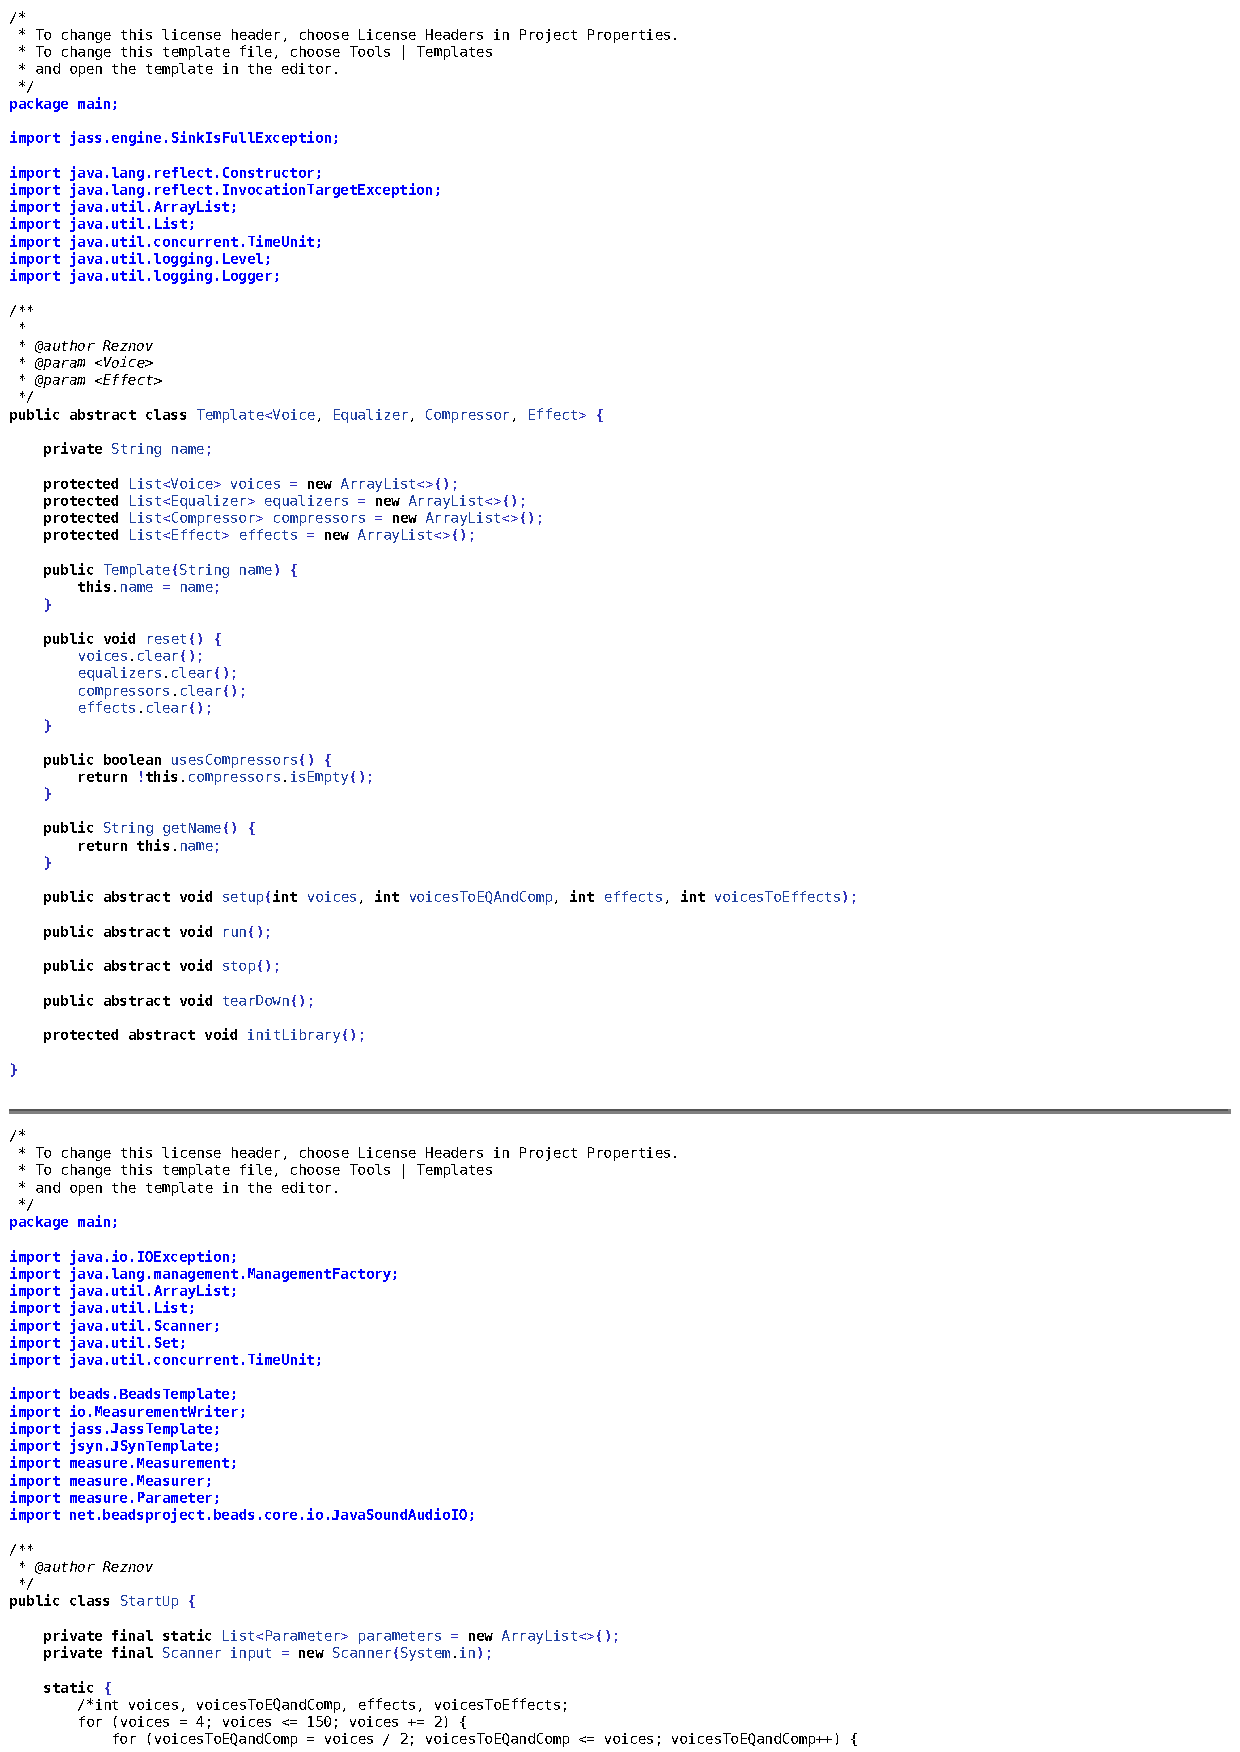
\includepdf[pages=-]{codepdfs/main.pdf}
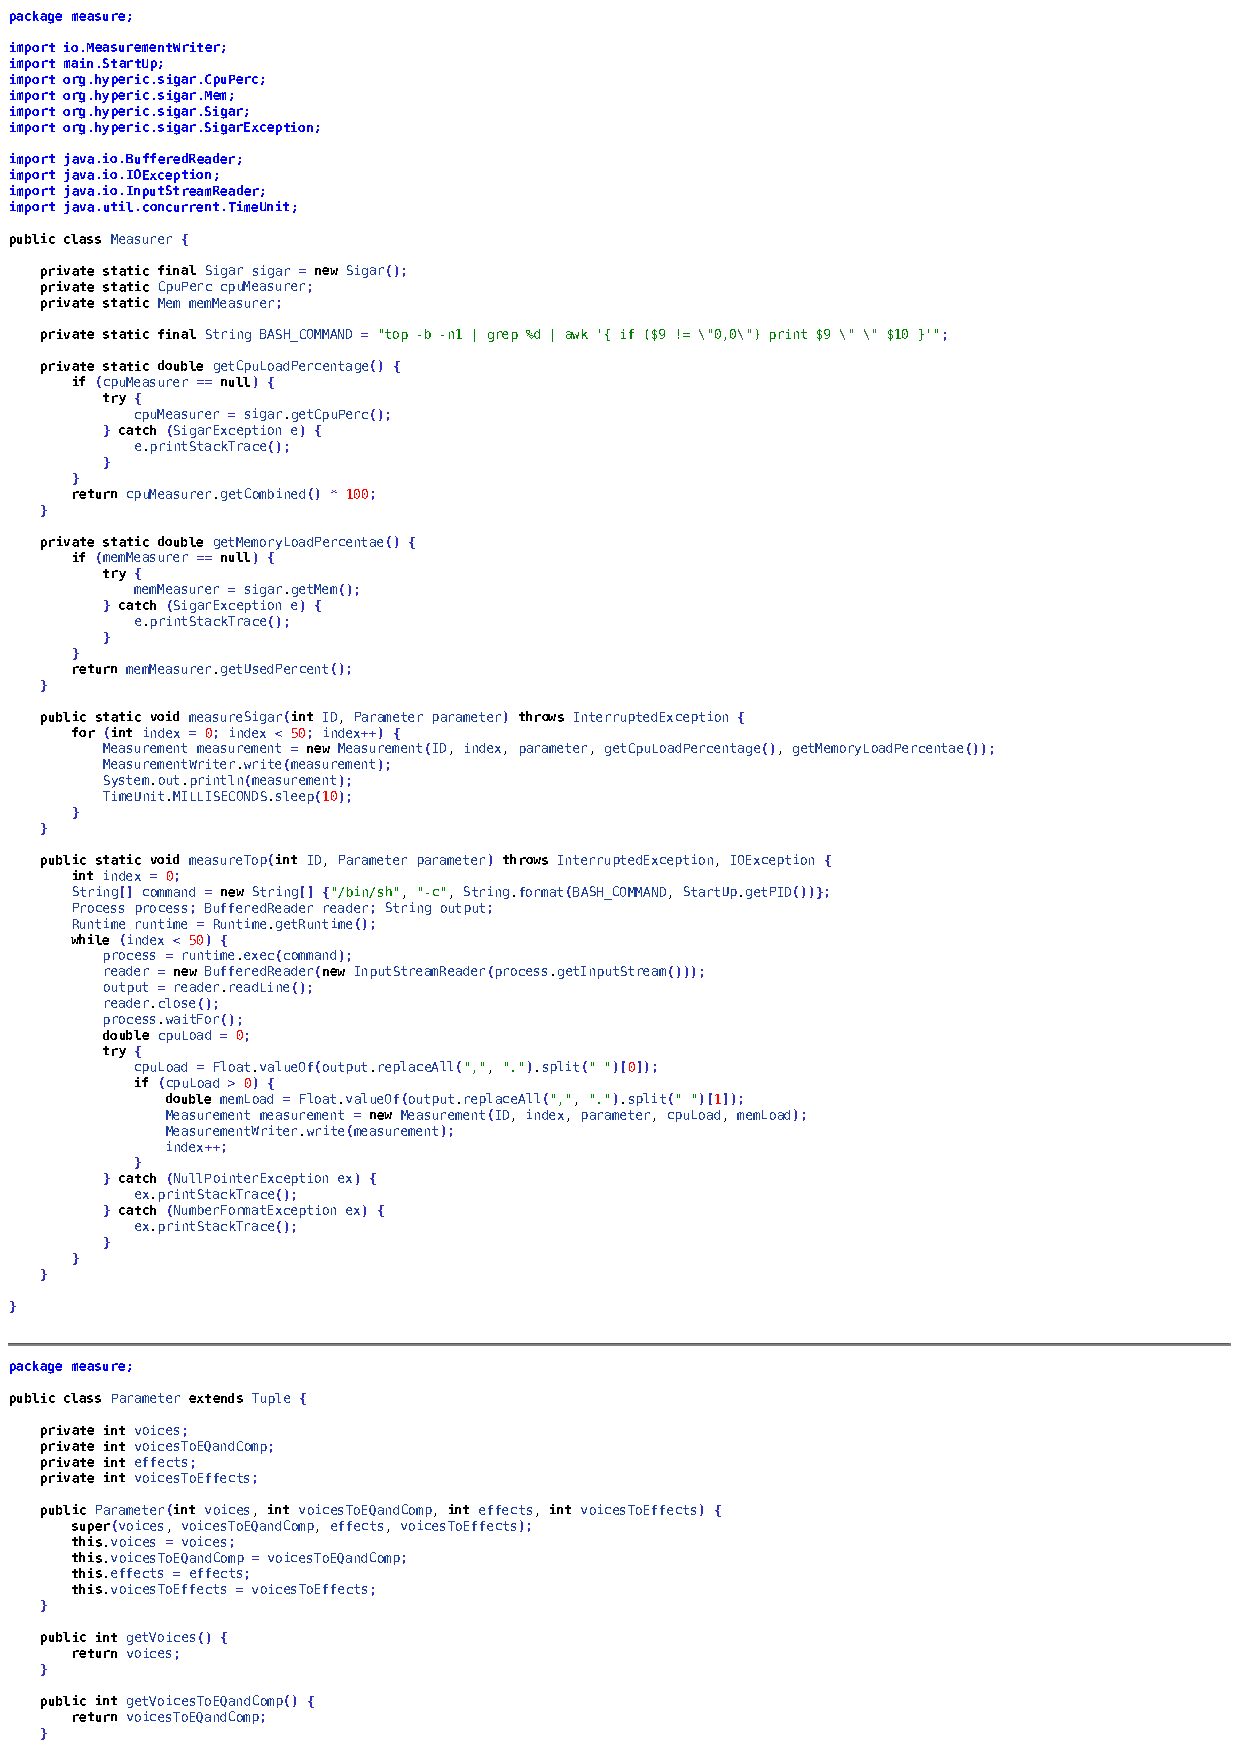
\includepdf[pages=-]{codepdfs/measure.pdf}
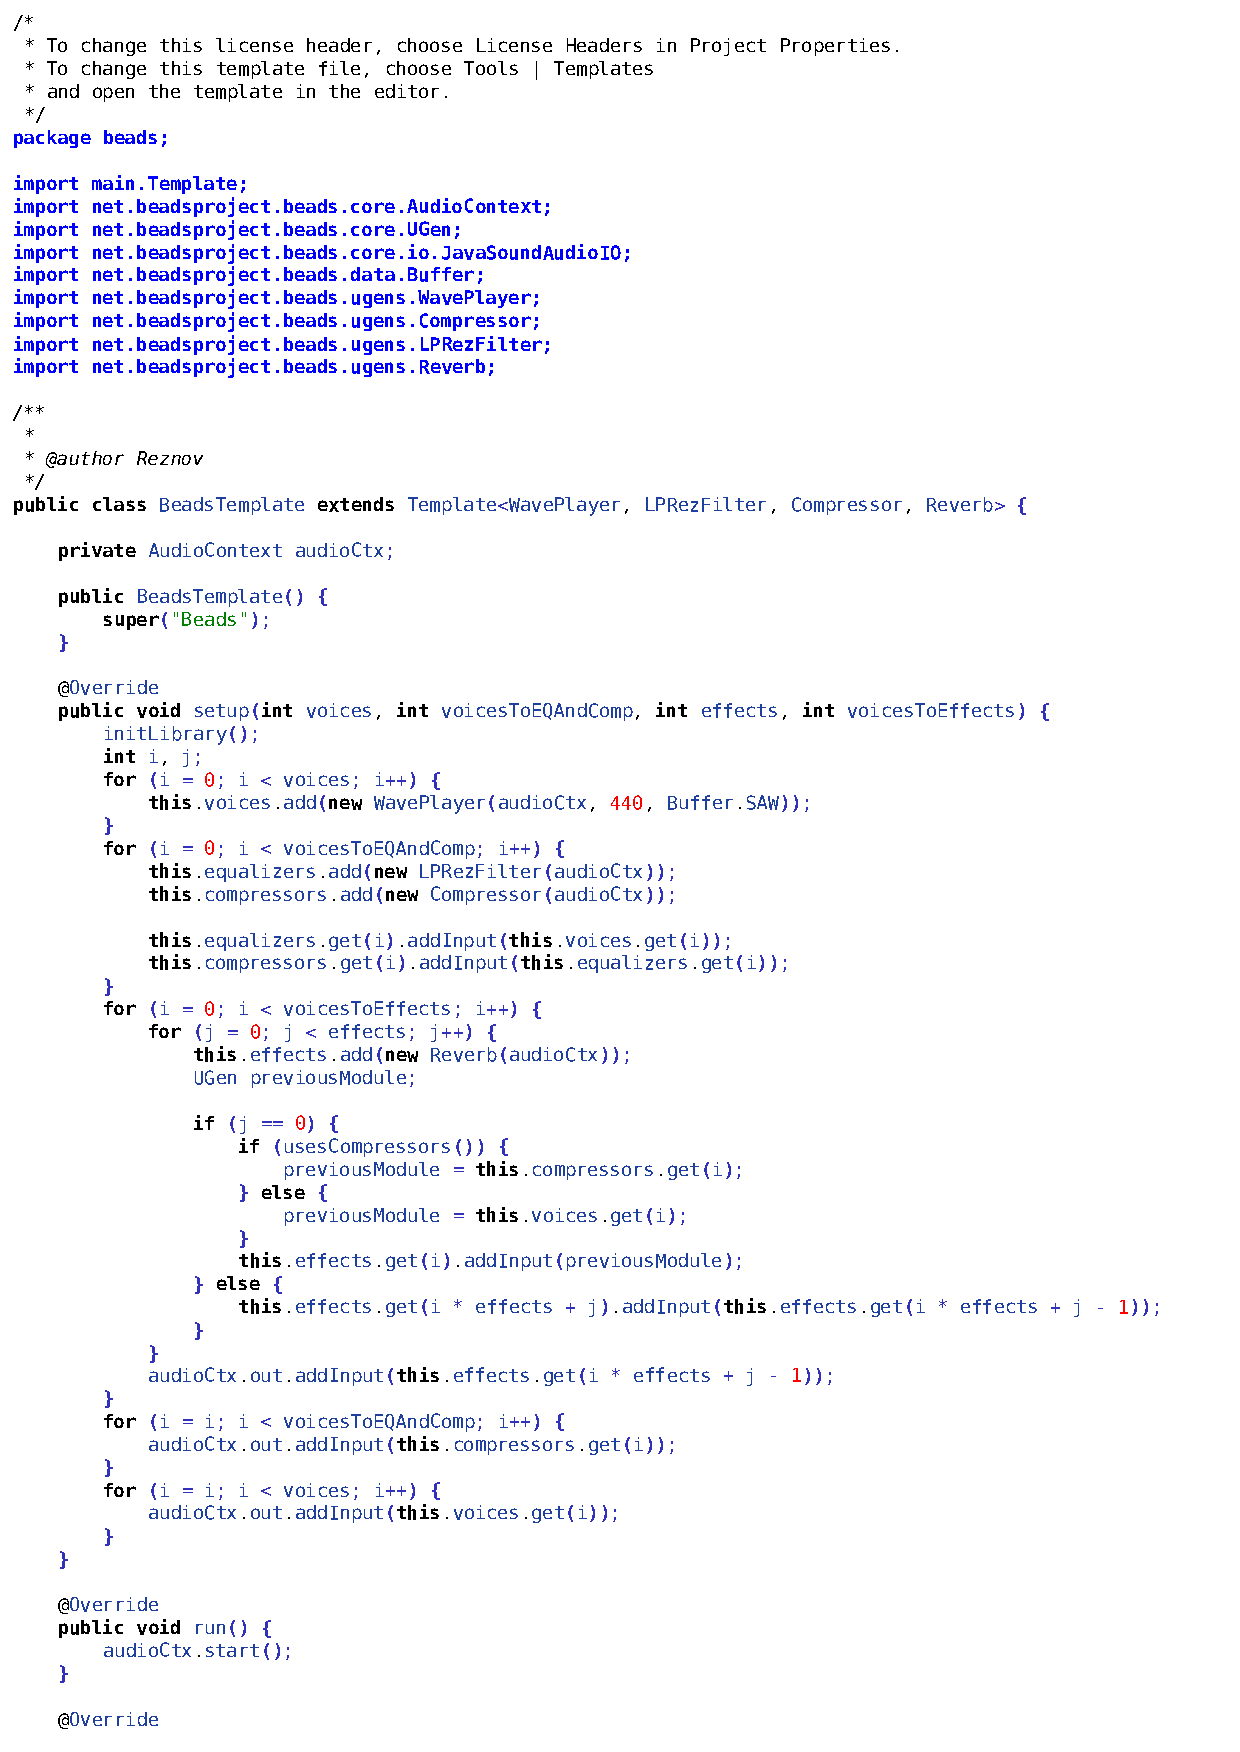
\includepdf[pages=-]{codepdfs/beads.pdf}
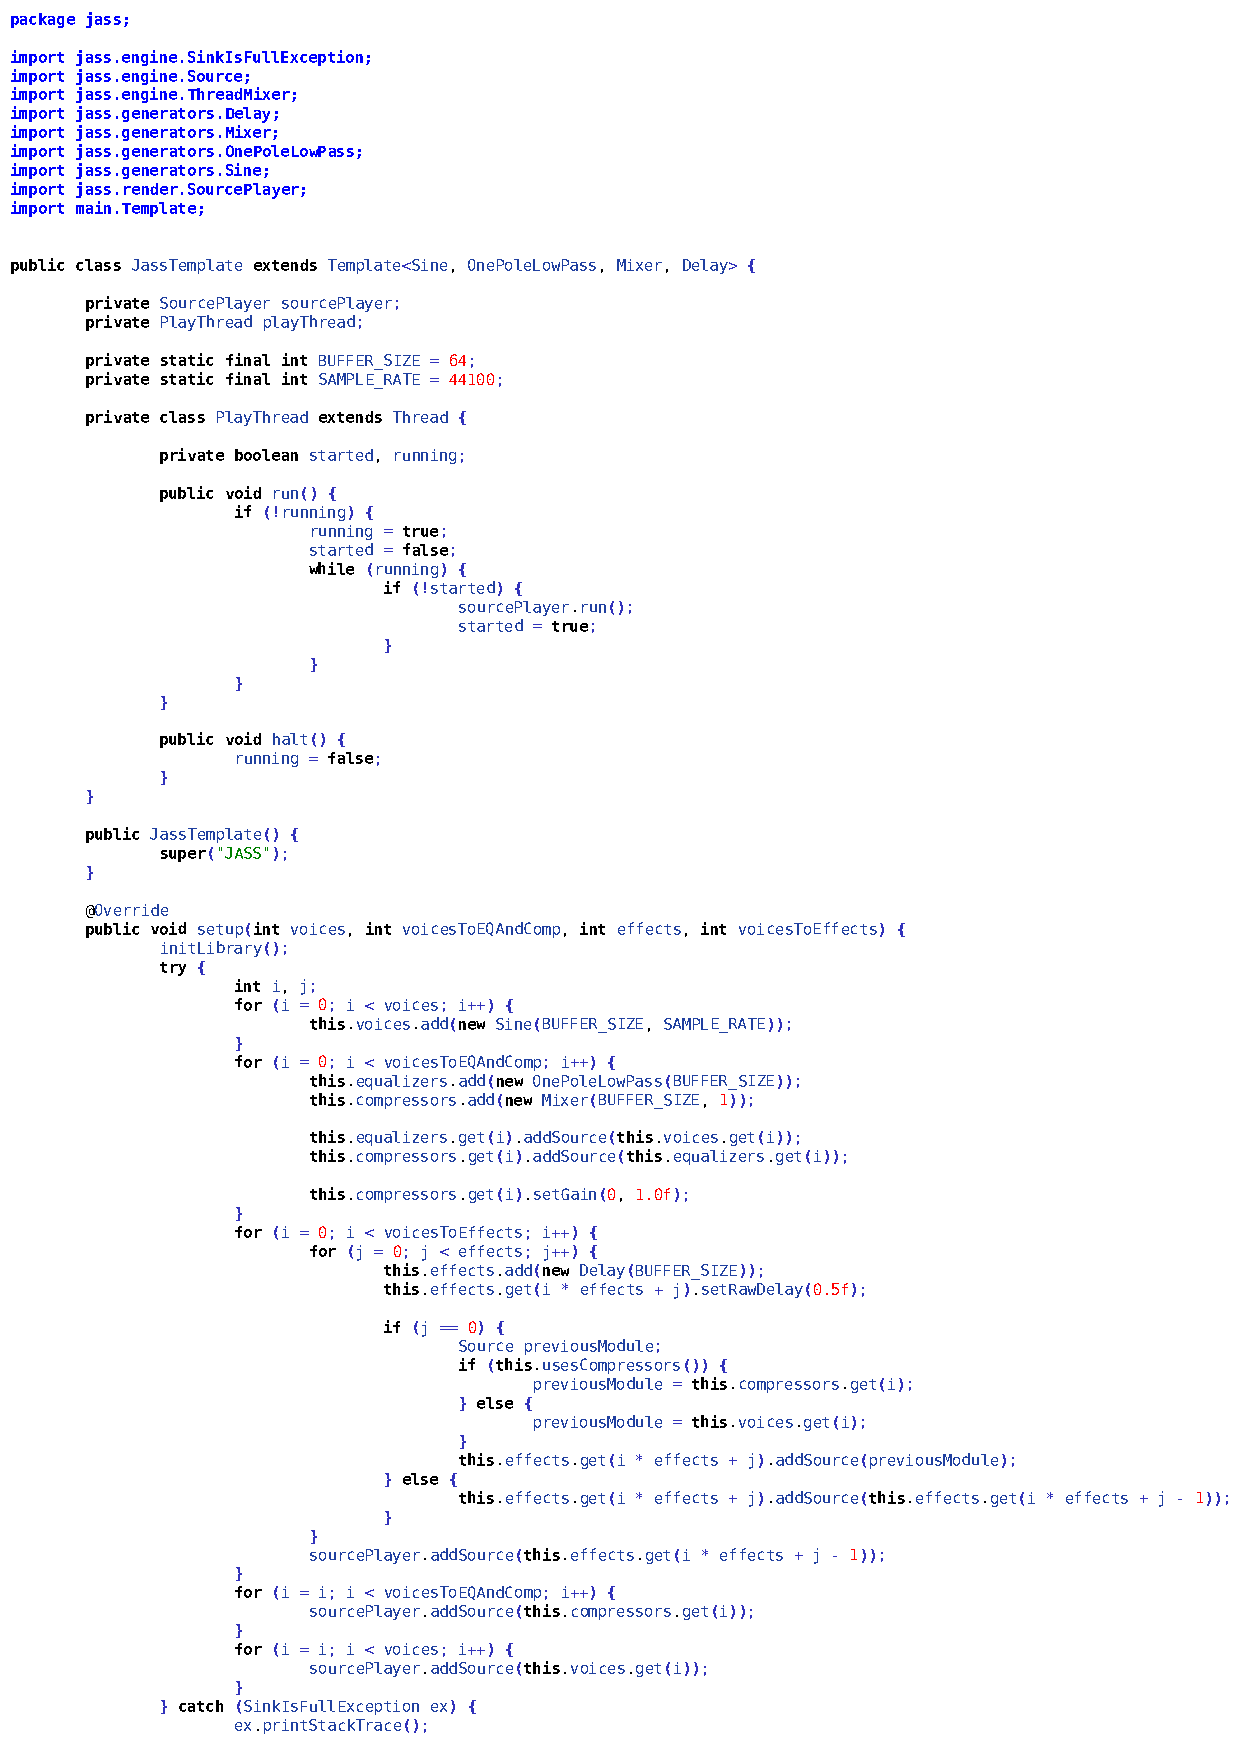
\includepdf[pages=-]{codepdfs/jass.pdf}
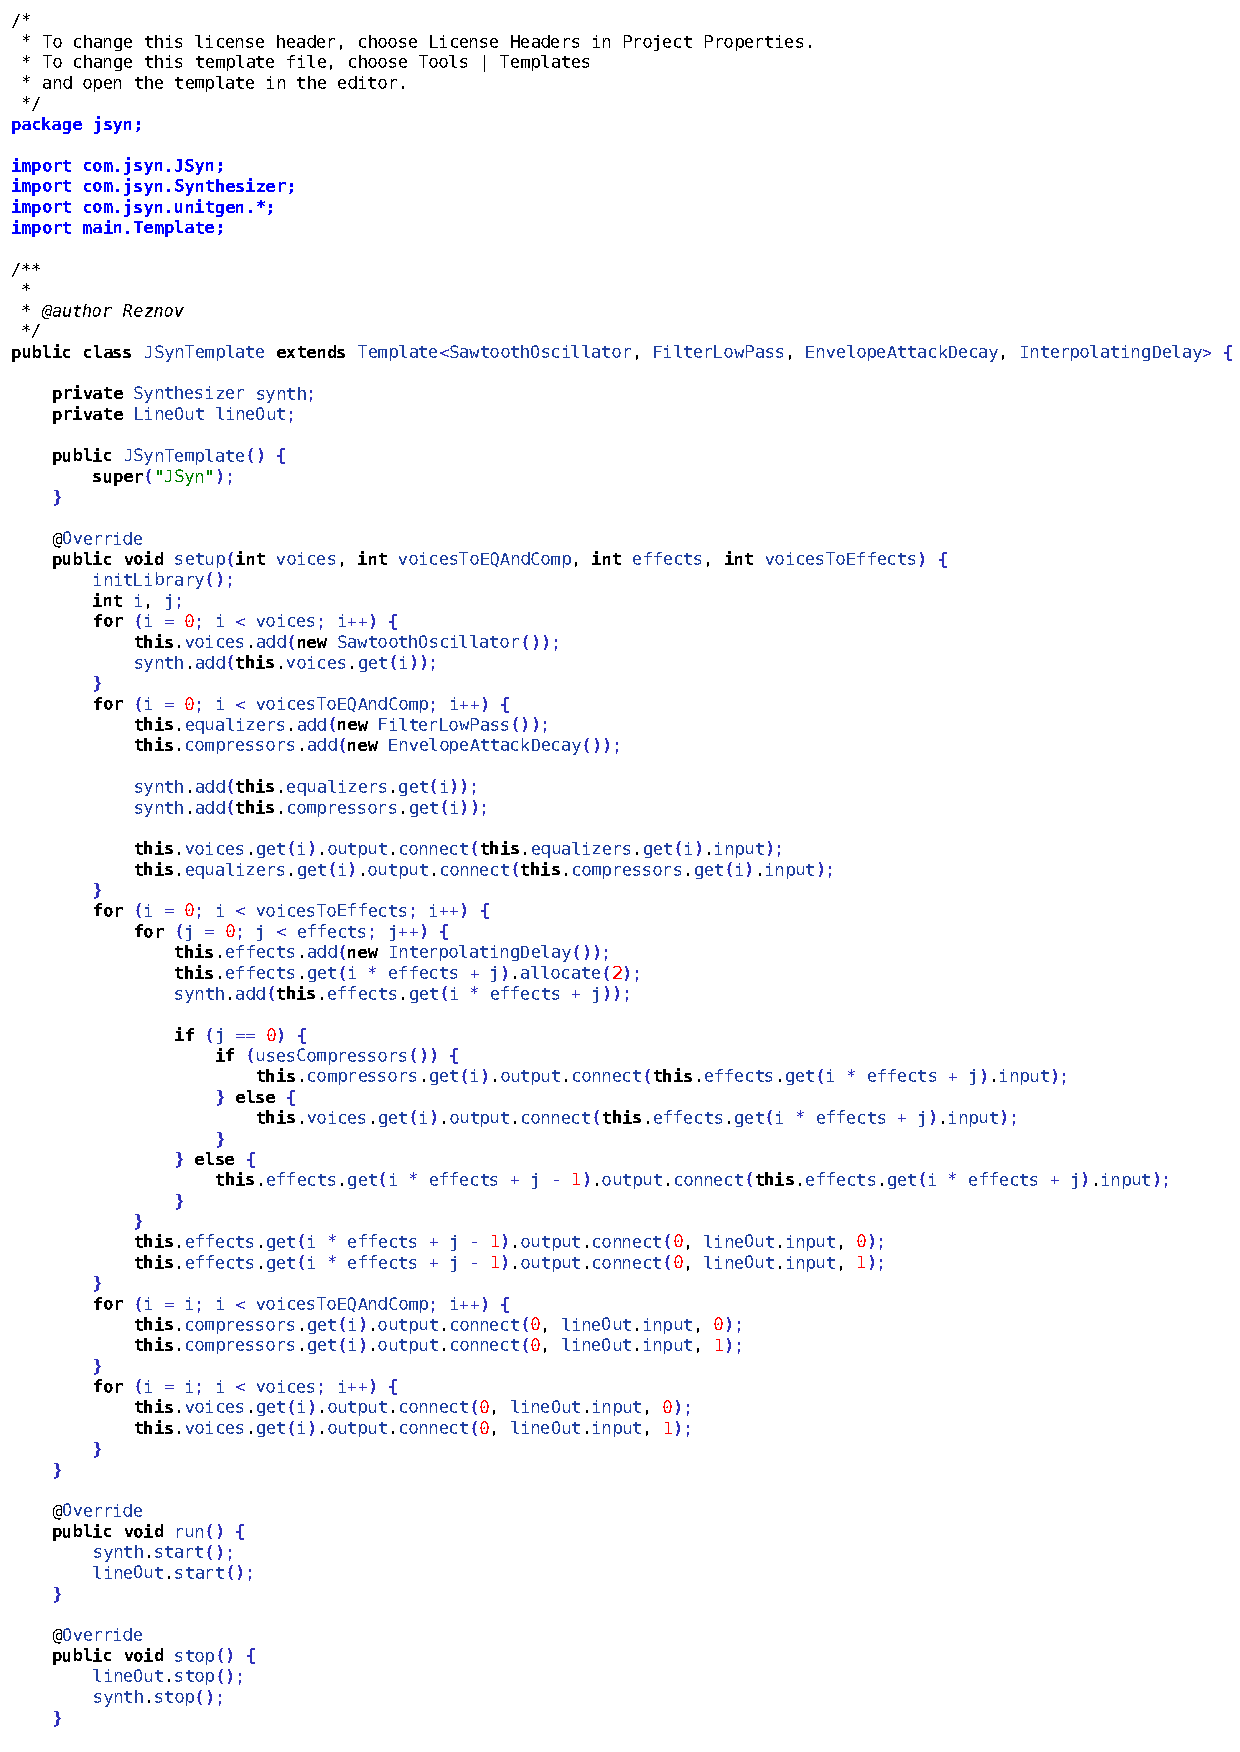
\includepdf[pages=-]{codepdfs/jsyn.pdf}
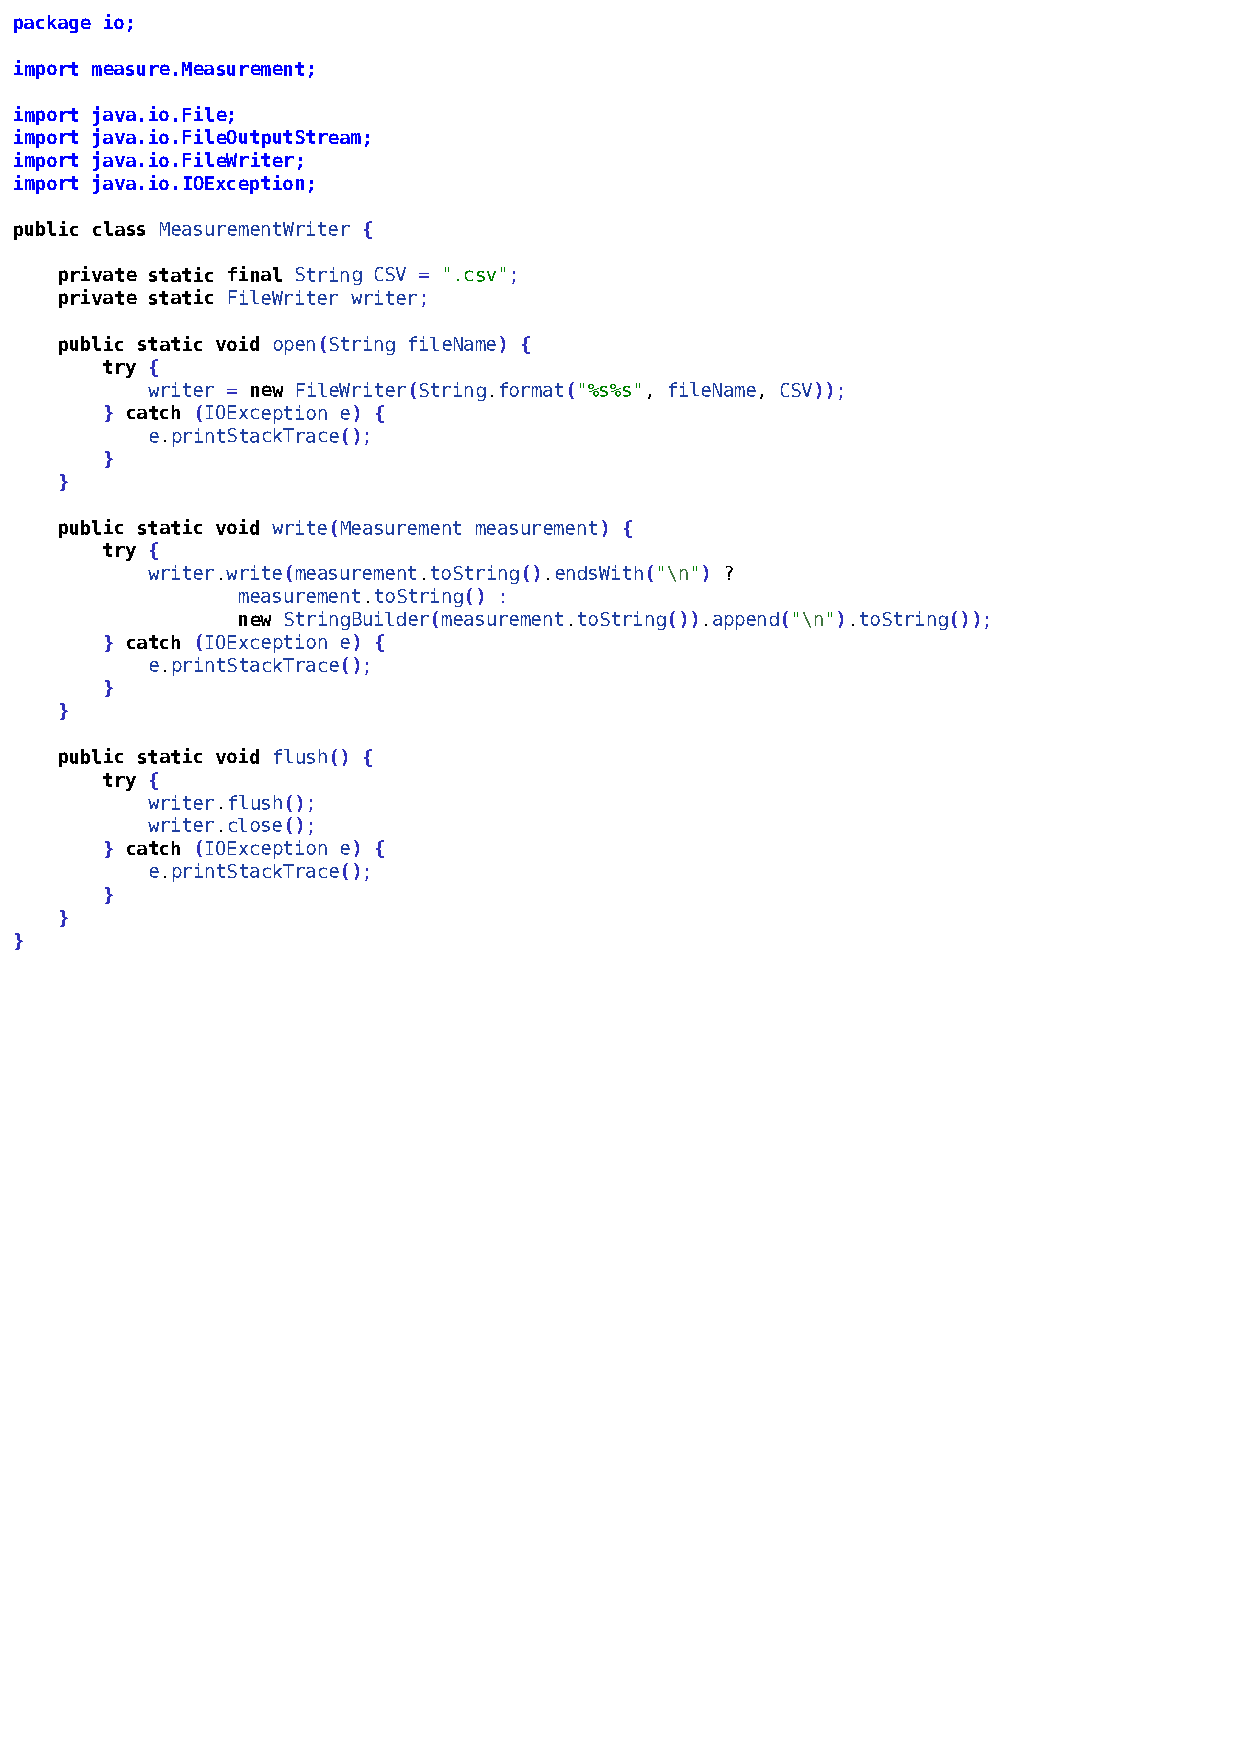
\includepdf[pages=-]{codepdfs/io.pdf}

\newcount\foo

\chapter{Testresultaten}
\label{ch:testresultaten}

\section{Testresultaten van Beads}

\foo=1
\loop
  
     \begin{longtable}[c]{|l|l|l|}
        \caption{Beads testresultaten van case \the\foo.}\\
        \hline
        \textbf{Index} & \textbf{\%CPU} & \textbf{\%Mem}\\
        \hline
        \csvreader[
            column count = 50,
            late after line = \\]
        {csvs/beads\the\foo.csv}
        {2=\index,7=\CPUPerc,8=\MemPerc}
        {\index & \CPUPerc & \MemPerc}
    \end{longtable}
  
  \advance \foo +1
\ifnum \foo<7
\repeat

\section{Testresultaten van JASS}

\foo=1
\loop
  
      \begin{longtable}[c]{|l|l|l|}
        \caption{JASS testresultaten van case \the\foo.}\\
        \hline
        \textbf{Index} & \textbf{\%CPU} & \textbf{\%Mem}\\
        \hline
        \csvreader[
            column count = 50,
            late after line = \\]
        {csvs/jass\the\foo.csv}
        {2=\index,7=\CPUPerc,8=\MemPerc}
        {\index & \CPUPerc & \MemPerc}
    \end{longtable}
  
  \advance \foo +1
\ifnum \foo<7
\repeat

\section{Testresultaten van JSyn}

\foo=1
\loop
  
      \begin{longtable}[c]{|l|l|l|}
        \caption{JSyn testresultaten van case \the\foo.}\\
        \hline
        \textbf{Index} & \textbf{\%CPU} & \textbf{\%Mem}\\
        \hline
        \csvreader[
            column count = 50,
            late after line = \\]
        {csvs/jsyn\the\foo.csv}
        {2=\index,7=\CPUPerc,8=\MemPerc}
        {\index & \CPUPerc & \MemPerc}
    \end{longtable}
  
  \advance \foo +1
\ifnum \foo<7
\repeat



\newcount\foo

\chapter{Smoothing van de Testresultaten}
\label{ch:smoothing}

\section{Smoothing van CPU testresultaten voor Beads}

\foo=1
\loop
    
    \begin{figure}
    		\centering
    		\includegraphics[width=0.75\linewidth]{medians/beads_cpu_\the\foo}
    		\caption{Smoothing van CPU testresultaten van testcase \the\foo  voor Beads}
    \end{figure}
  
  \advance \foo +1
\ifnum \foo<6
\repeat

\section{Smoothing van Mem testresultaten voor Beads}

\foo=1
\loop
    
    \begin{figure}
    		\centering
    		\includegraphics[width=0.75\linewidth]{medians/beads_mem_\the\foo}
    		\caption{Smoothing van Mem testresultaten van testcase \the\foo  voor Beads}
    \end{figure}
  
  \advance \foo +1
\ifnum \foo<6
\repeat

\section{Smoothing van CPU testresultaten voor JASS}

\foo=1
\loop
    
    \begin{figure}
    		\centering
    		\includegraphics[width=0.75\linewidth]{medians/jass_cpu_\the\foo}
    		\caption{Smoothing van CPU testresultaten van testcase \the\foo  voor JASS}
    \end{figure}
  
  \advance \foo +1
\ifnum \foo<6
\repeat

\section{Smoothing van Mem testresultaten voor JASS}

\foo=1
\loop
    
    \begin{figure}
    		\centering
    		\includegraphics[width=0.75\linewidth]{medians/jass_mem_\the\foo}
    		\caption{Smoothing van Mem testresultaten van testcase \the\foo  voor JASS}
    \end{figure}
  
  \advance \foo +1
\ifnum \foo<6
\repeat

\section{Smoothing van CPU testresultaten voor JSyn}

\foo=1
\loop
    
    \begin{figure}
    		\centering
    		\includegraphics[width=0.75\linewidth]{medians/jsyn_cpu_\the\foo}
    		\caption{Smoothing van CPU testresultaten van testcase \the\foo  voor JSyn}
    \end{figure}
  
  \advance \foo +1
\ifnum \foo<6
\repeat

\section{Smoothing van Mem testresultaten voor JSyn}

\foo=1
\loop
    
    \begin{figure}
    		\centering
    		\includegraphics[width=0.75\linewidth]{medians/jsyn_mem_\the\foo}
    		\caption{Smoothing van Mem testresultaten van testcase \the\foo  voor JSyn}
    \end{figure}
  
  \advance \foo +1
\ifnum \foo<6
\repeat


%%---------- Referentielijst --------------------------------------------------

\printbibliography[heading=bibintoc]

\end{document}
